 \documentclass[12pt]{article}
\usepackage{parskip}
\usepackage{pdfpages}
\usepackage[margin=.6in]{geometry}
\begin{document}
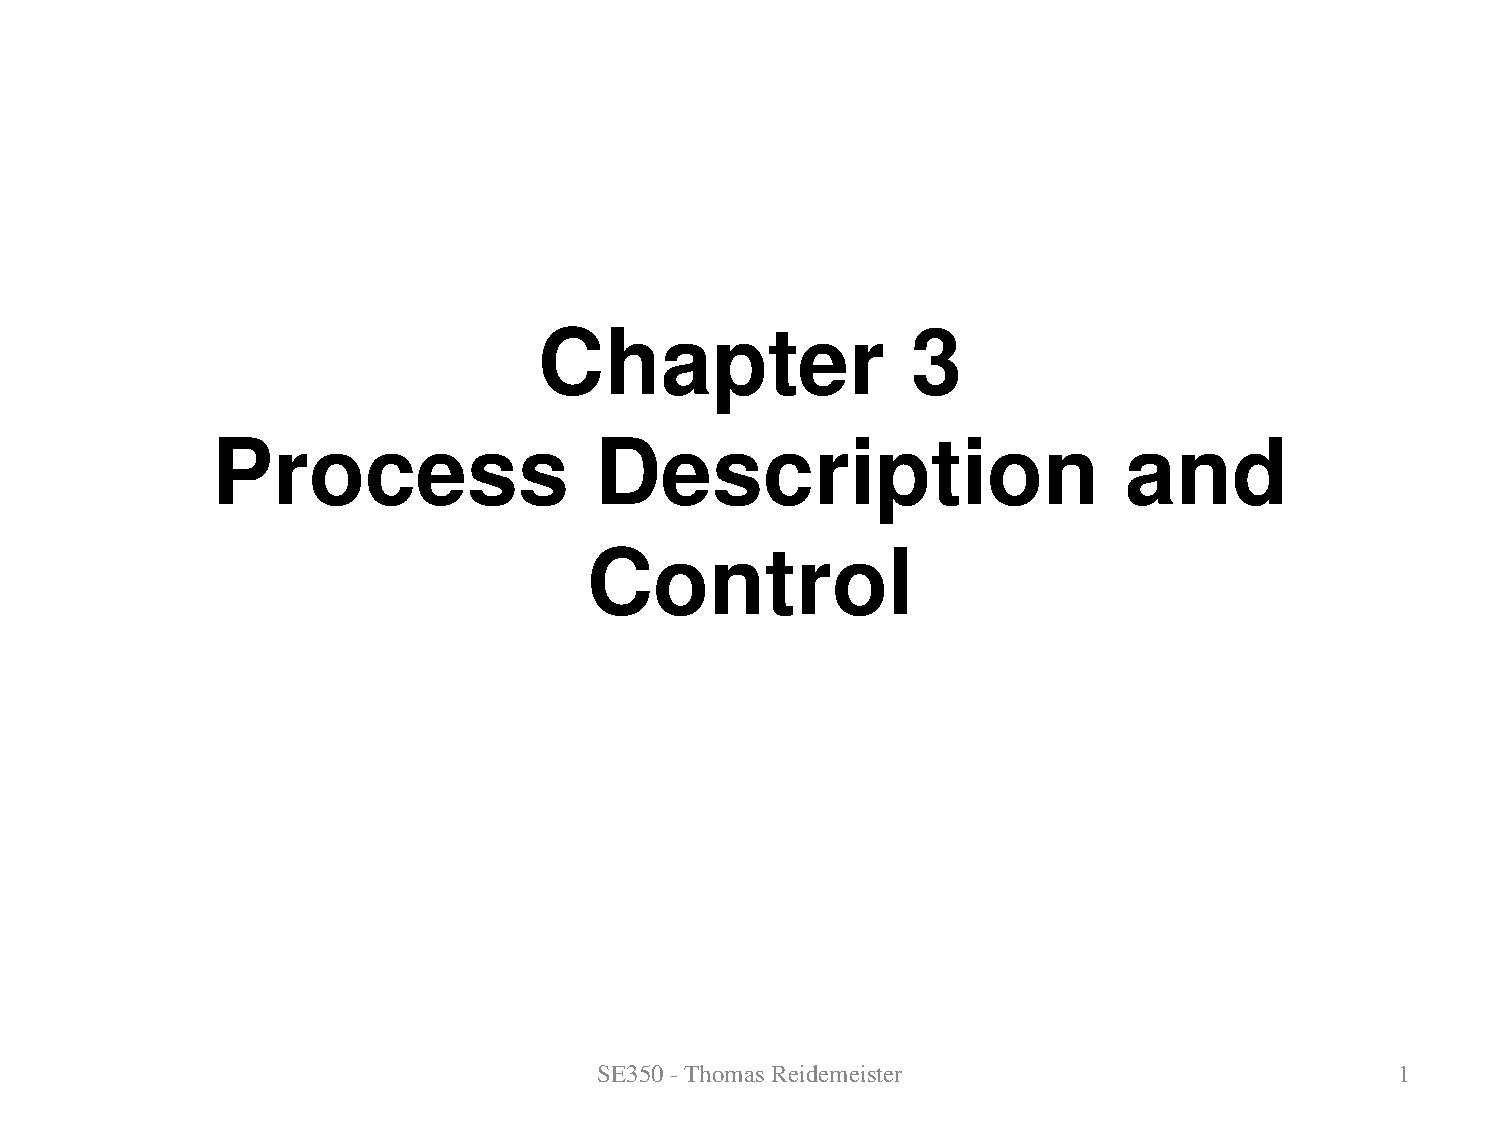
\includepdf[page=1]{03.pdf}
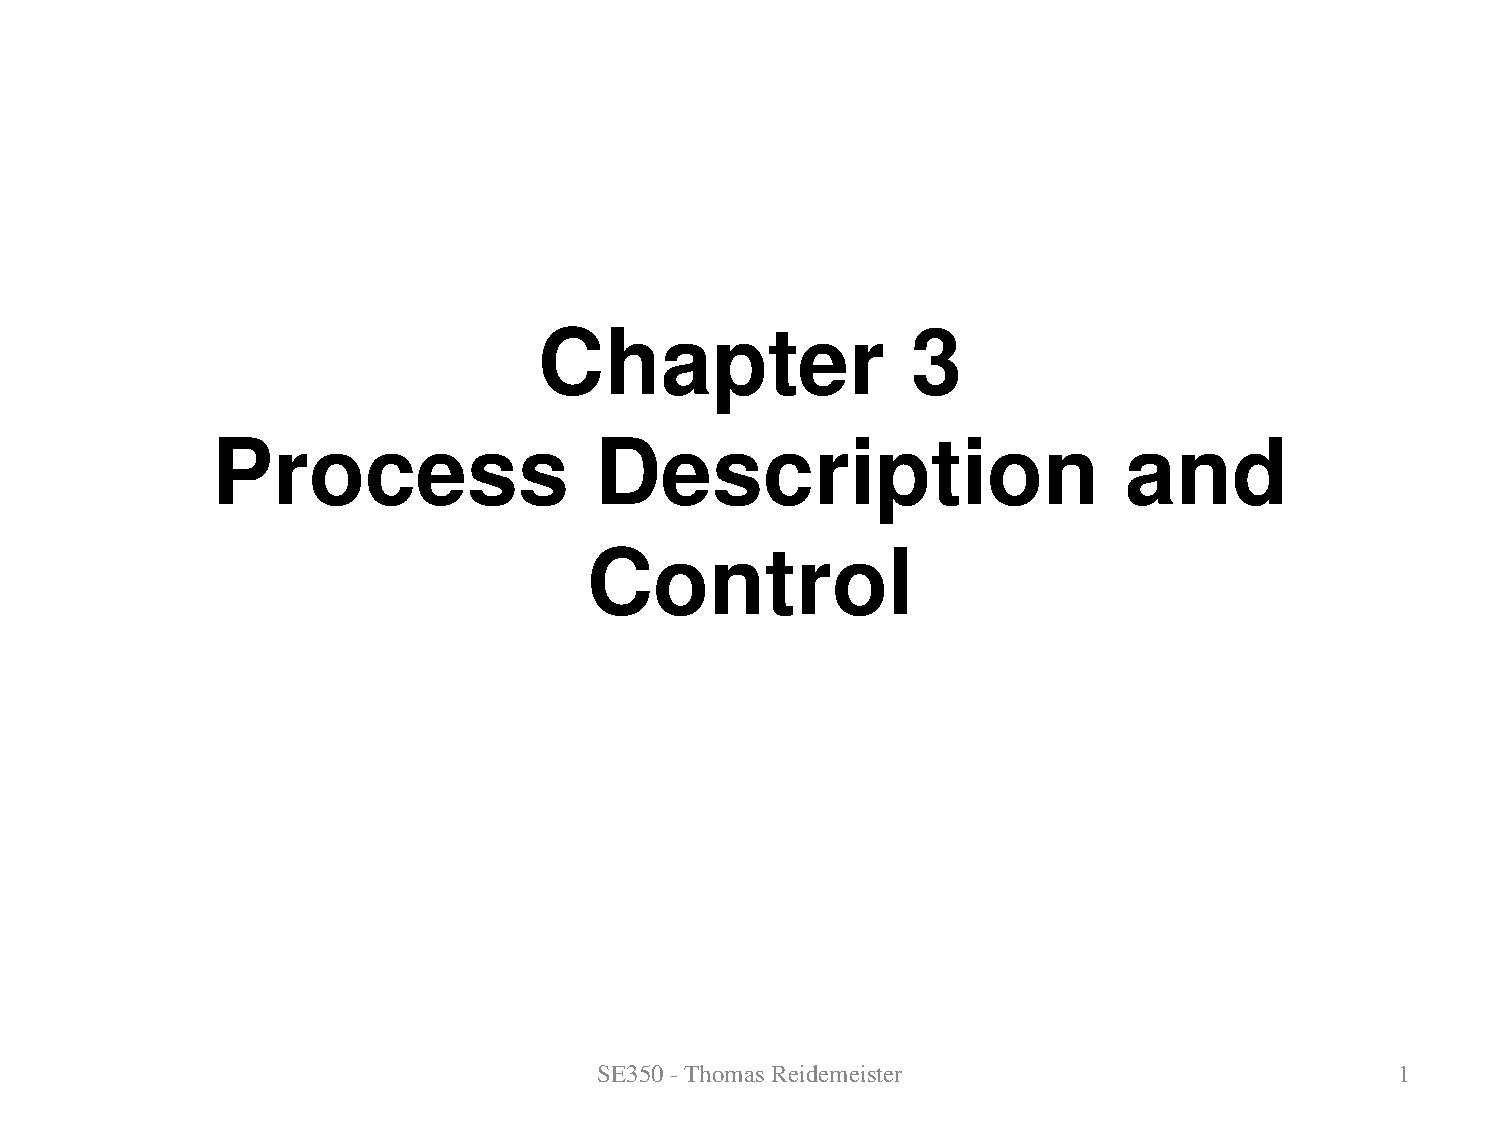
\includepdf[page=2]{03.pdf}
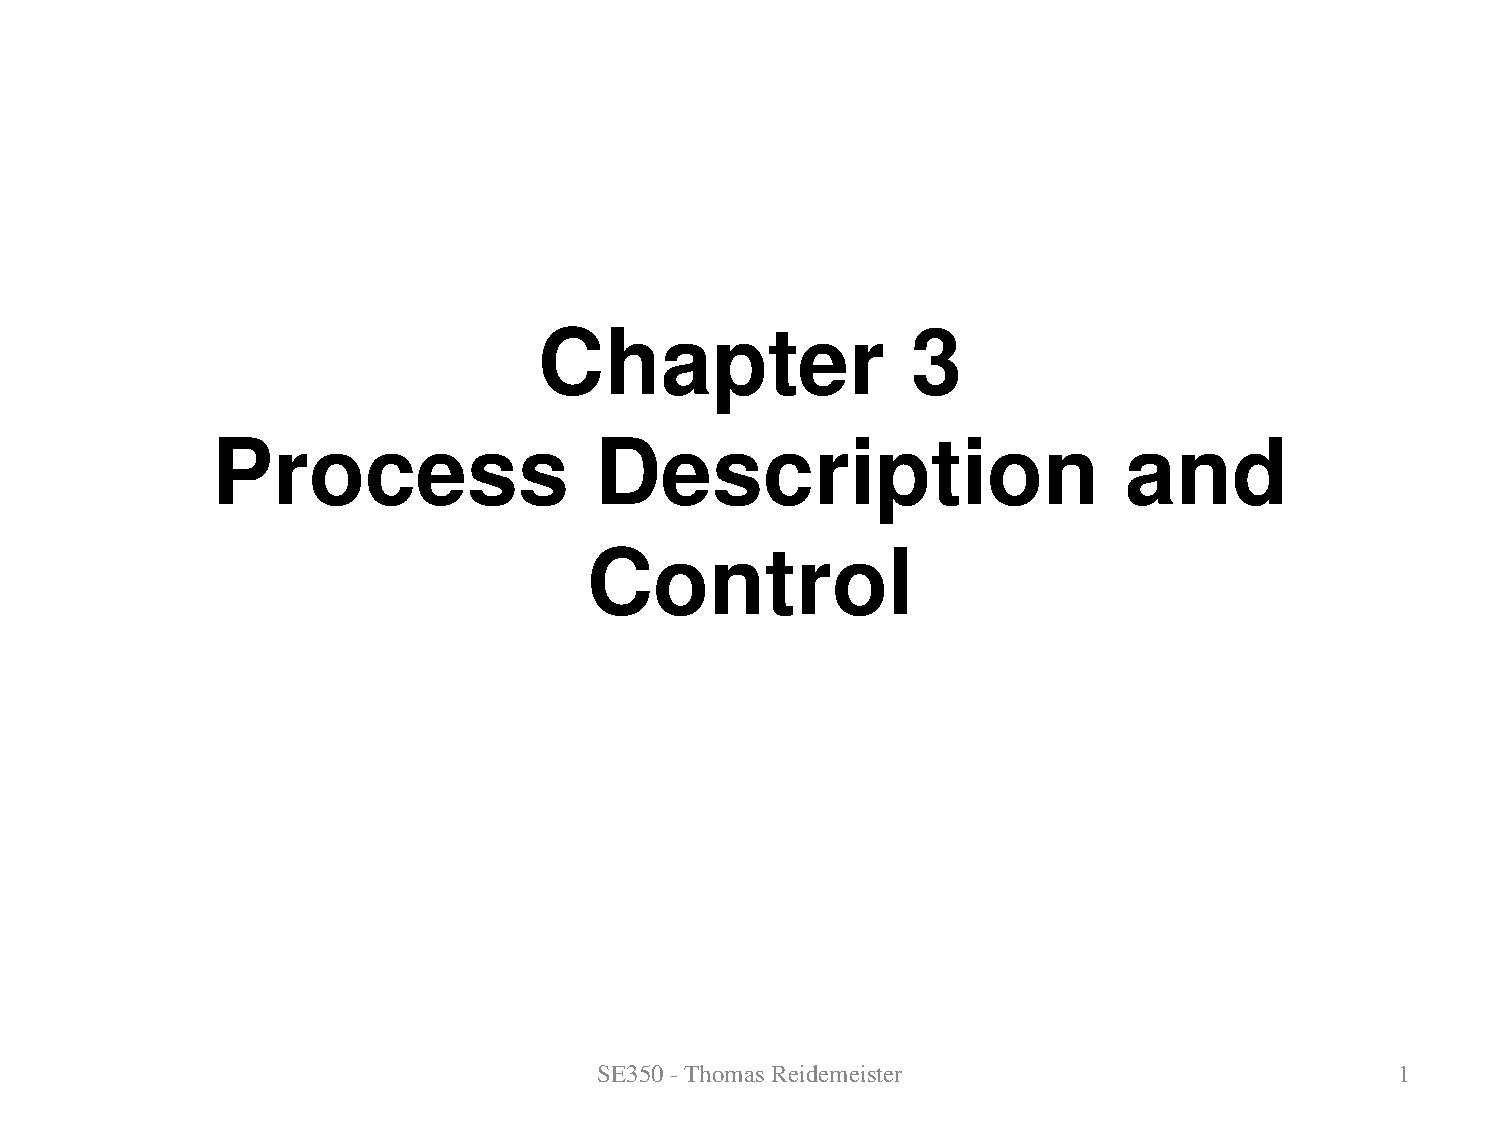
\includepdf[page=3]{03.pdf}
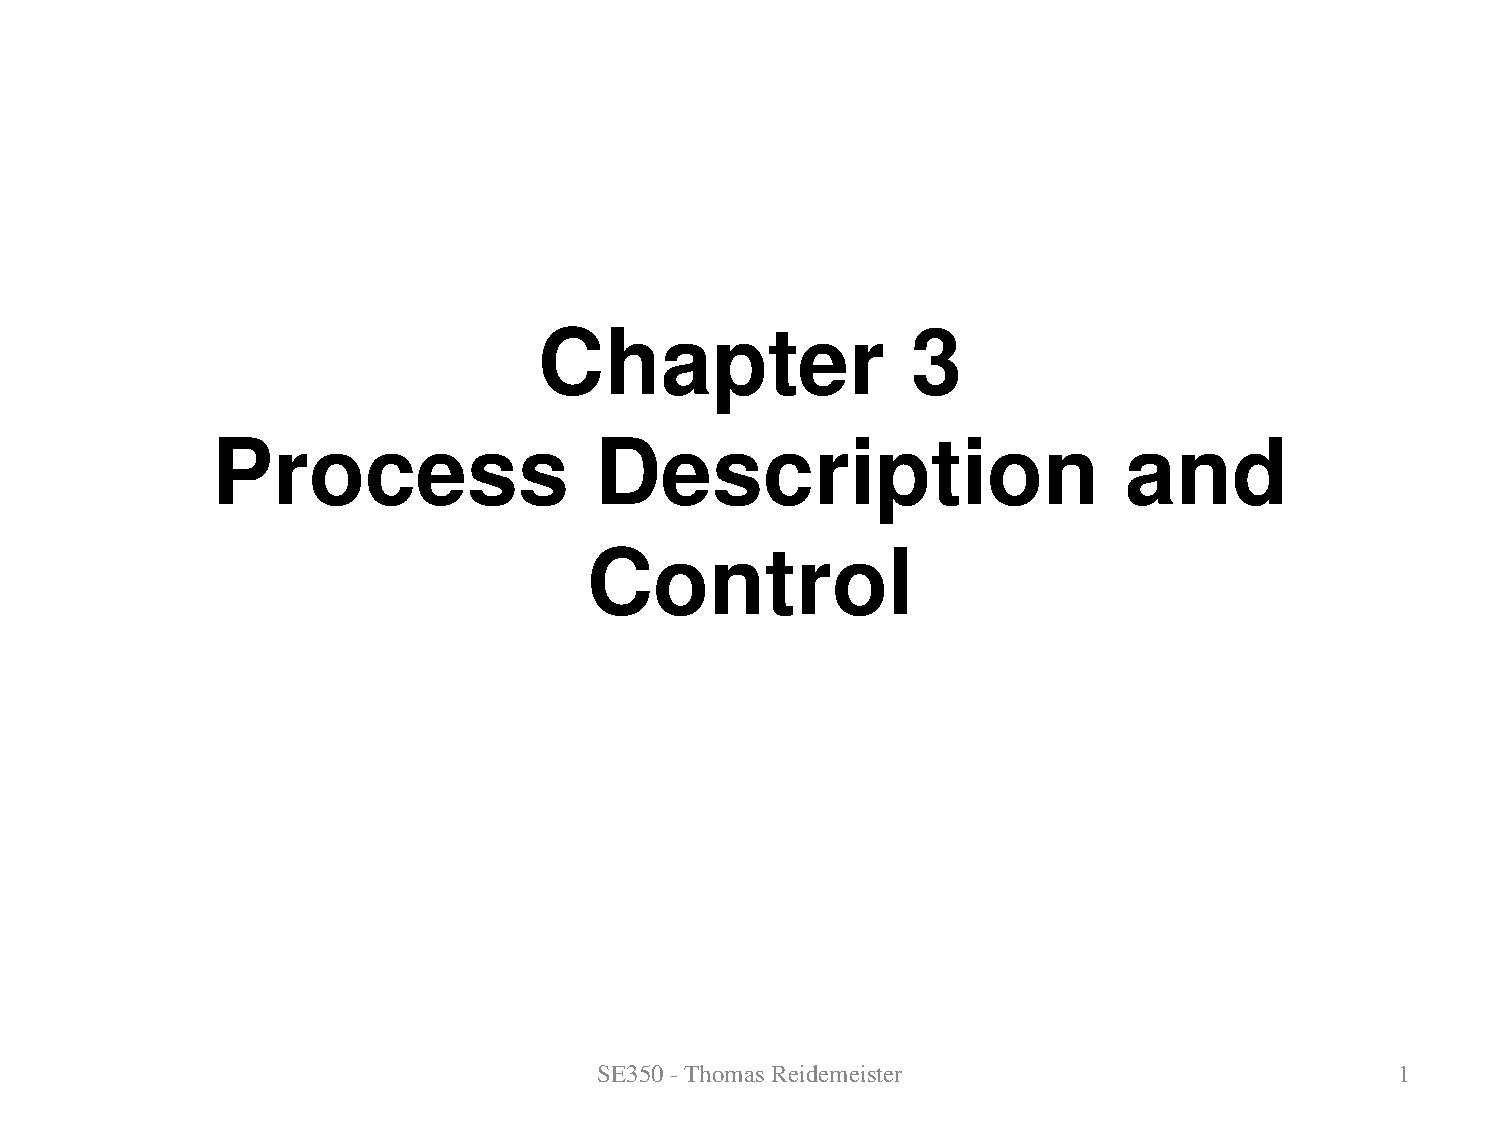
\includepdf[page=4]{03.pdf}
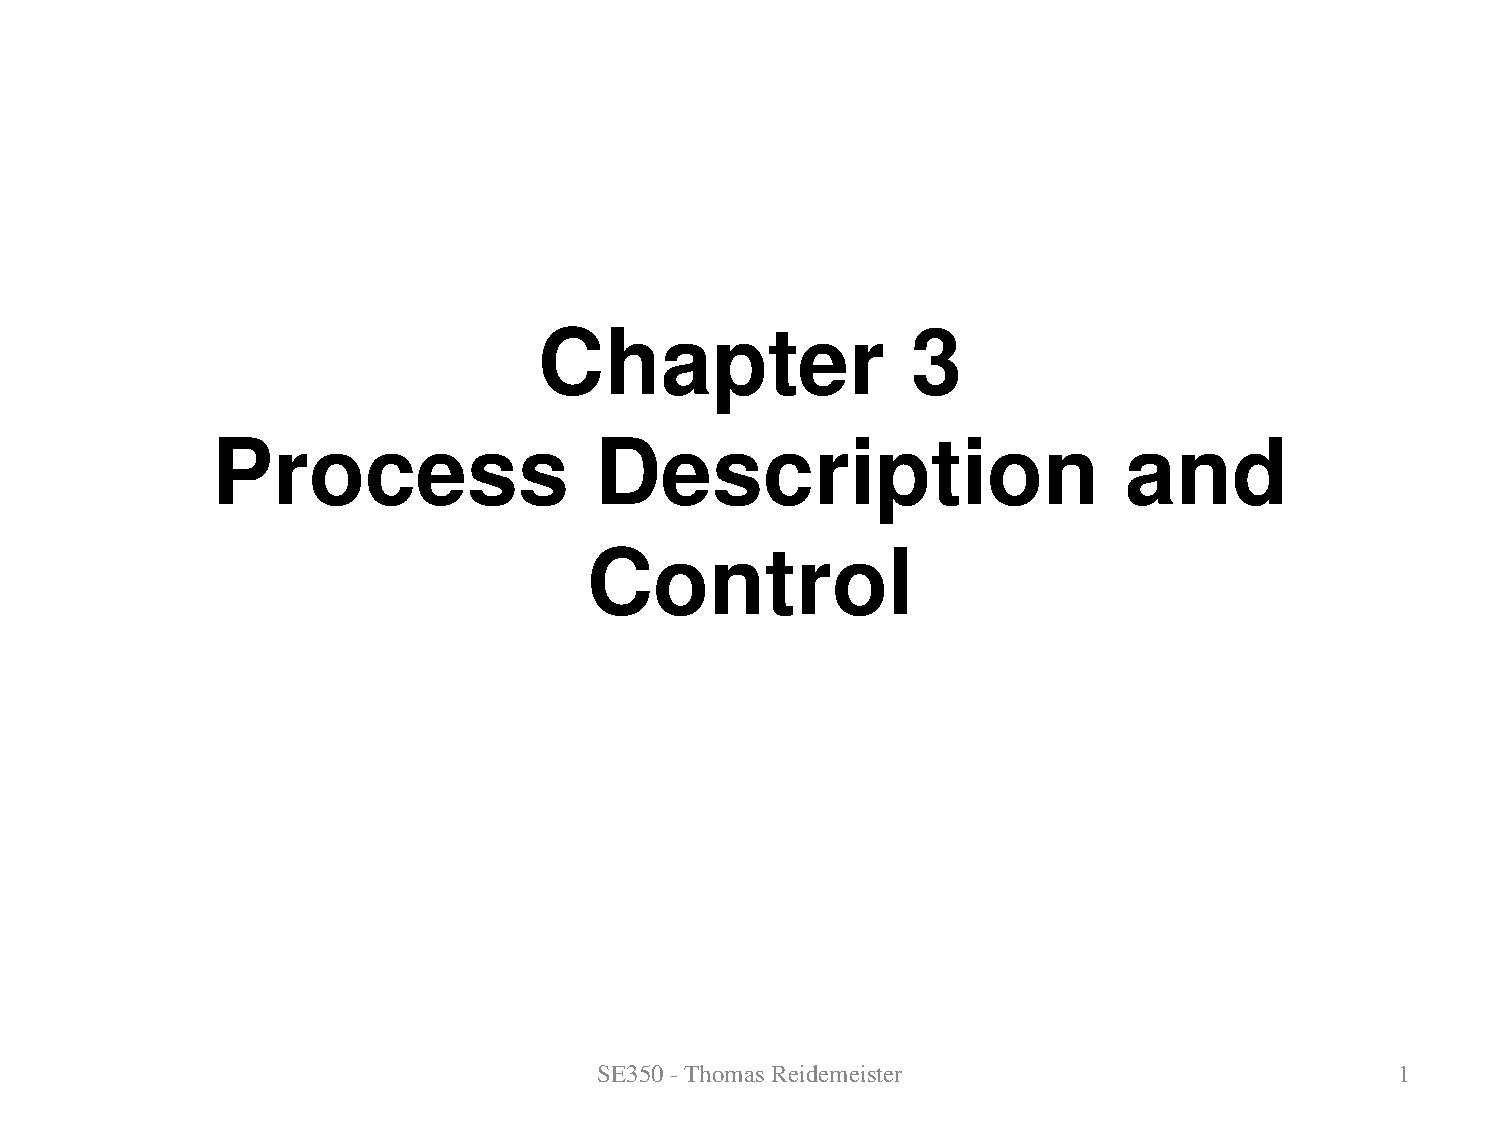
\includepdf[page=5]{03.pdf}
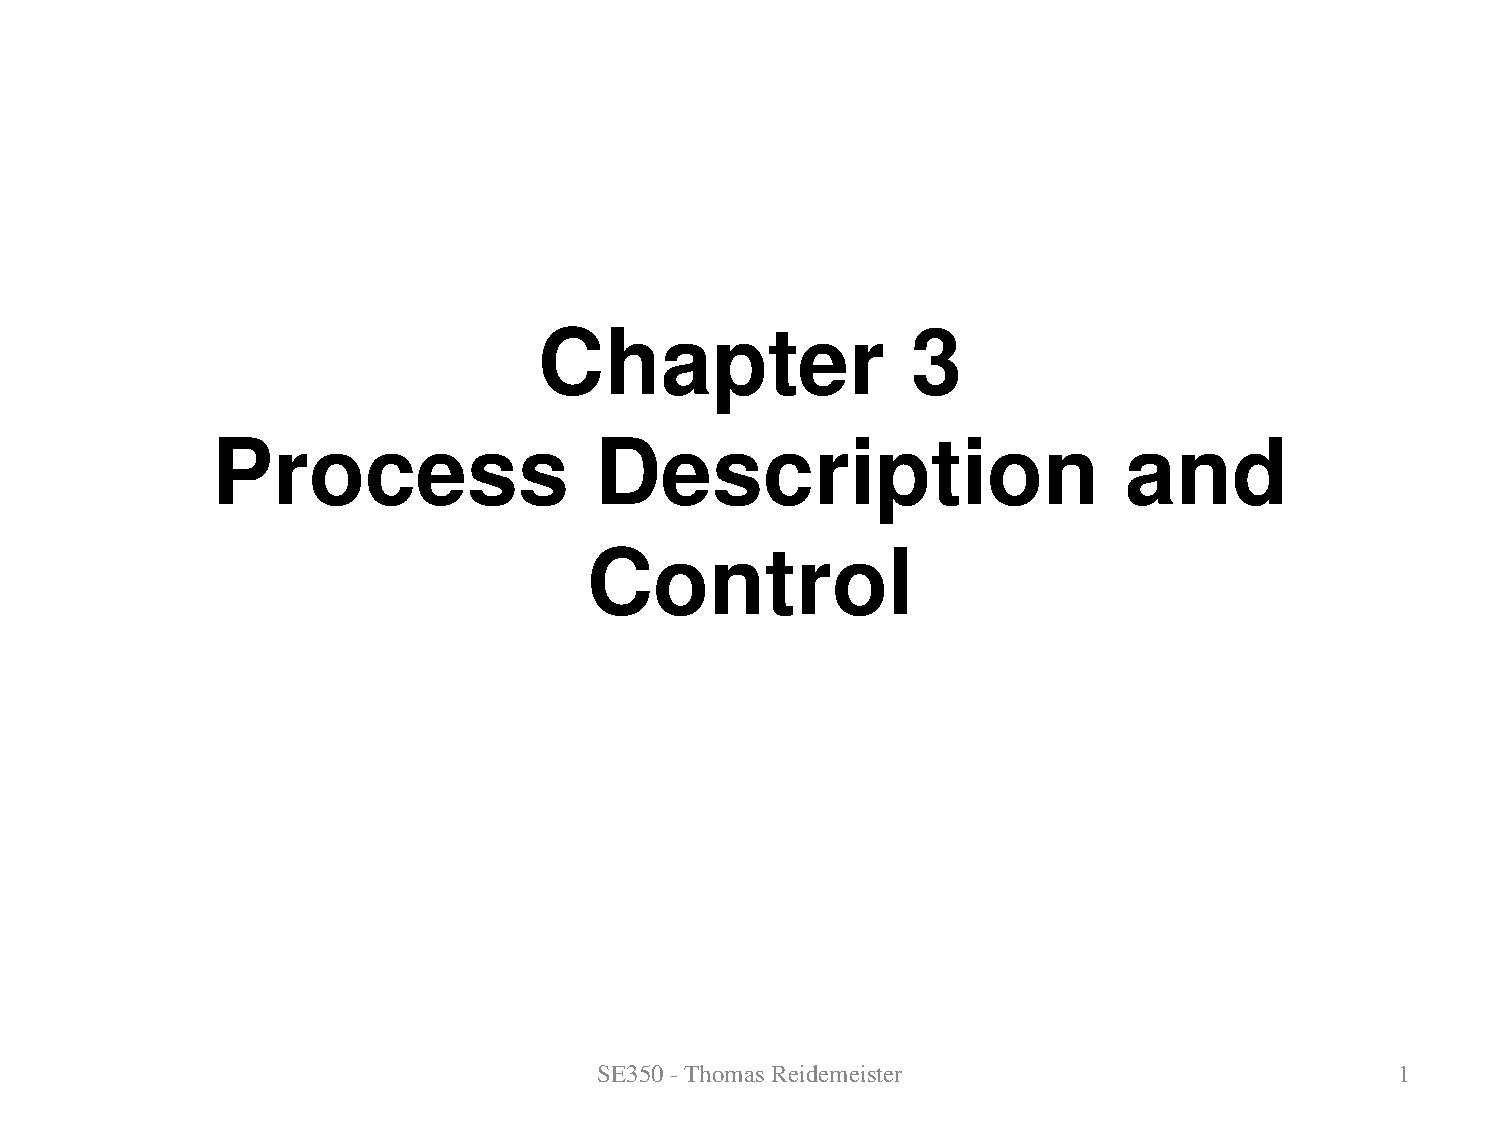
\includepdf[page=6]{03.pdf}
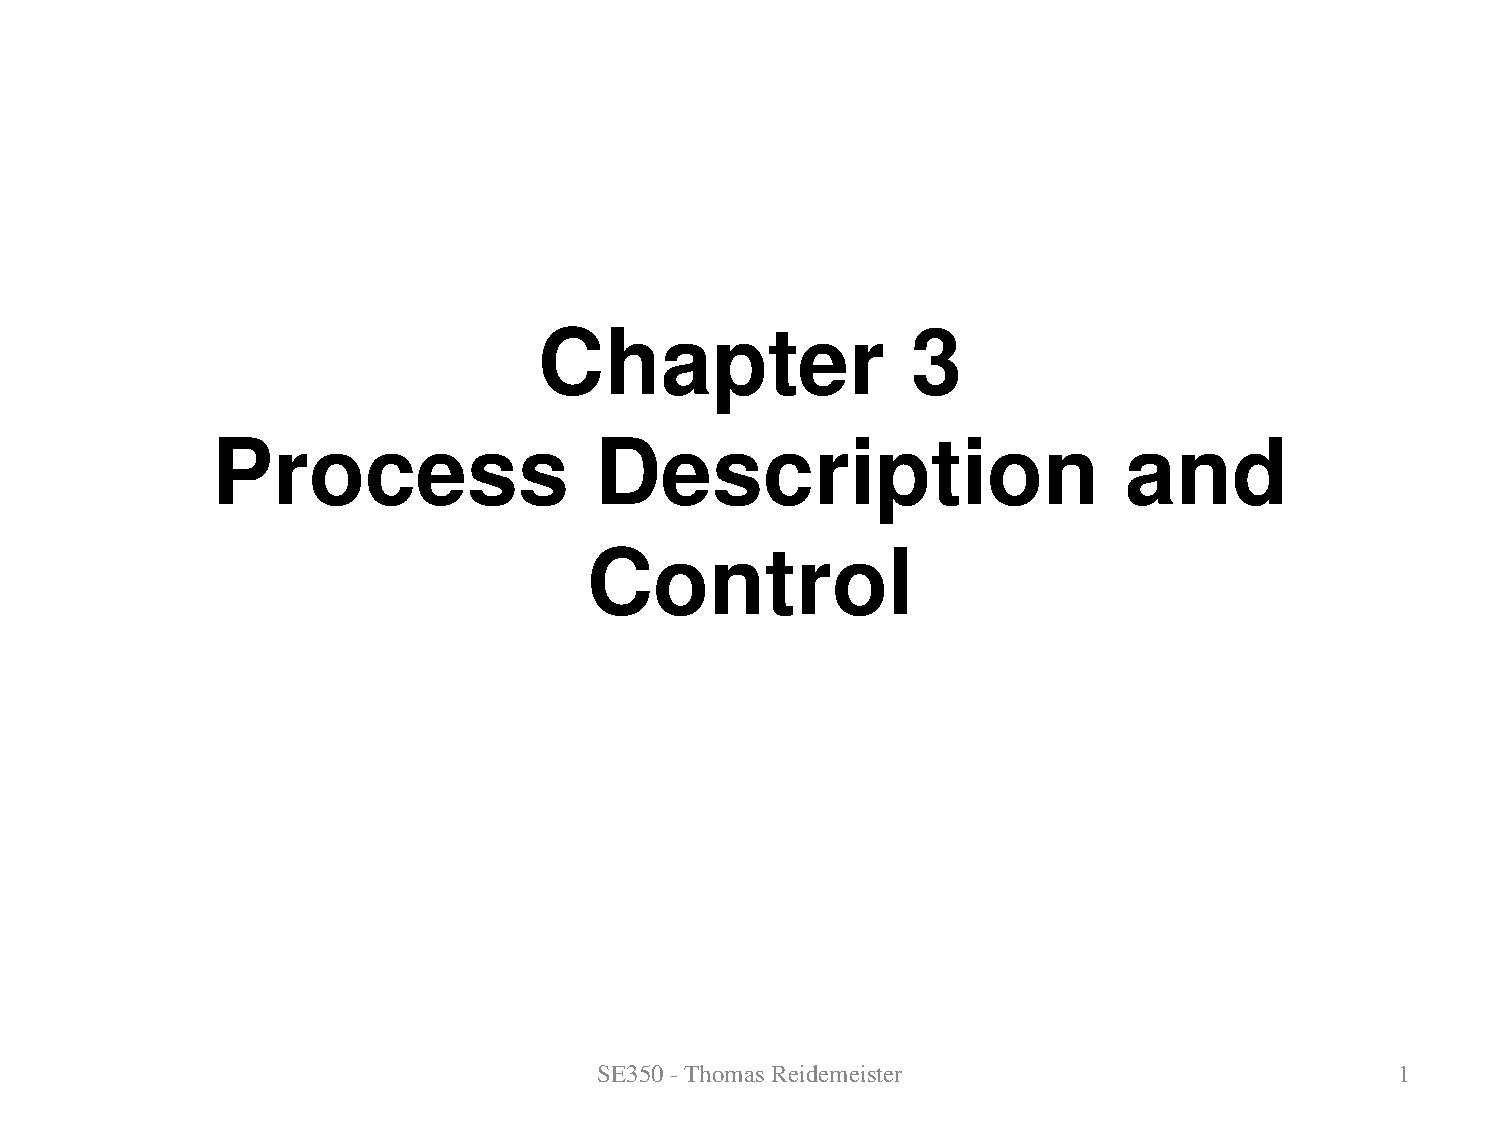
\includepdf[page=7]{03.pdf}
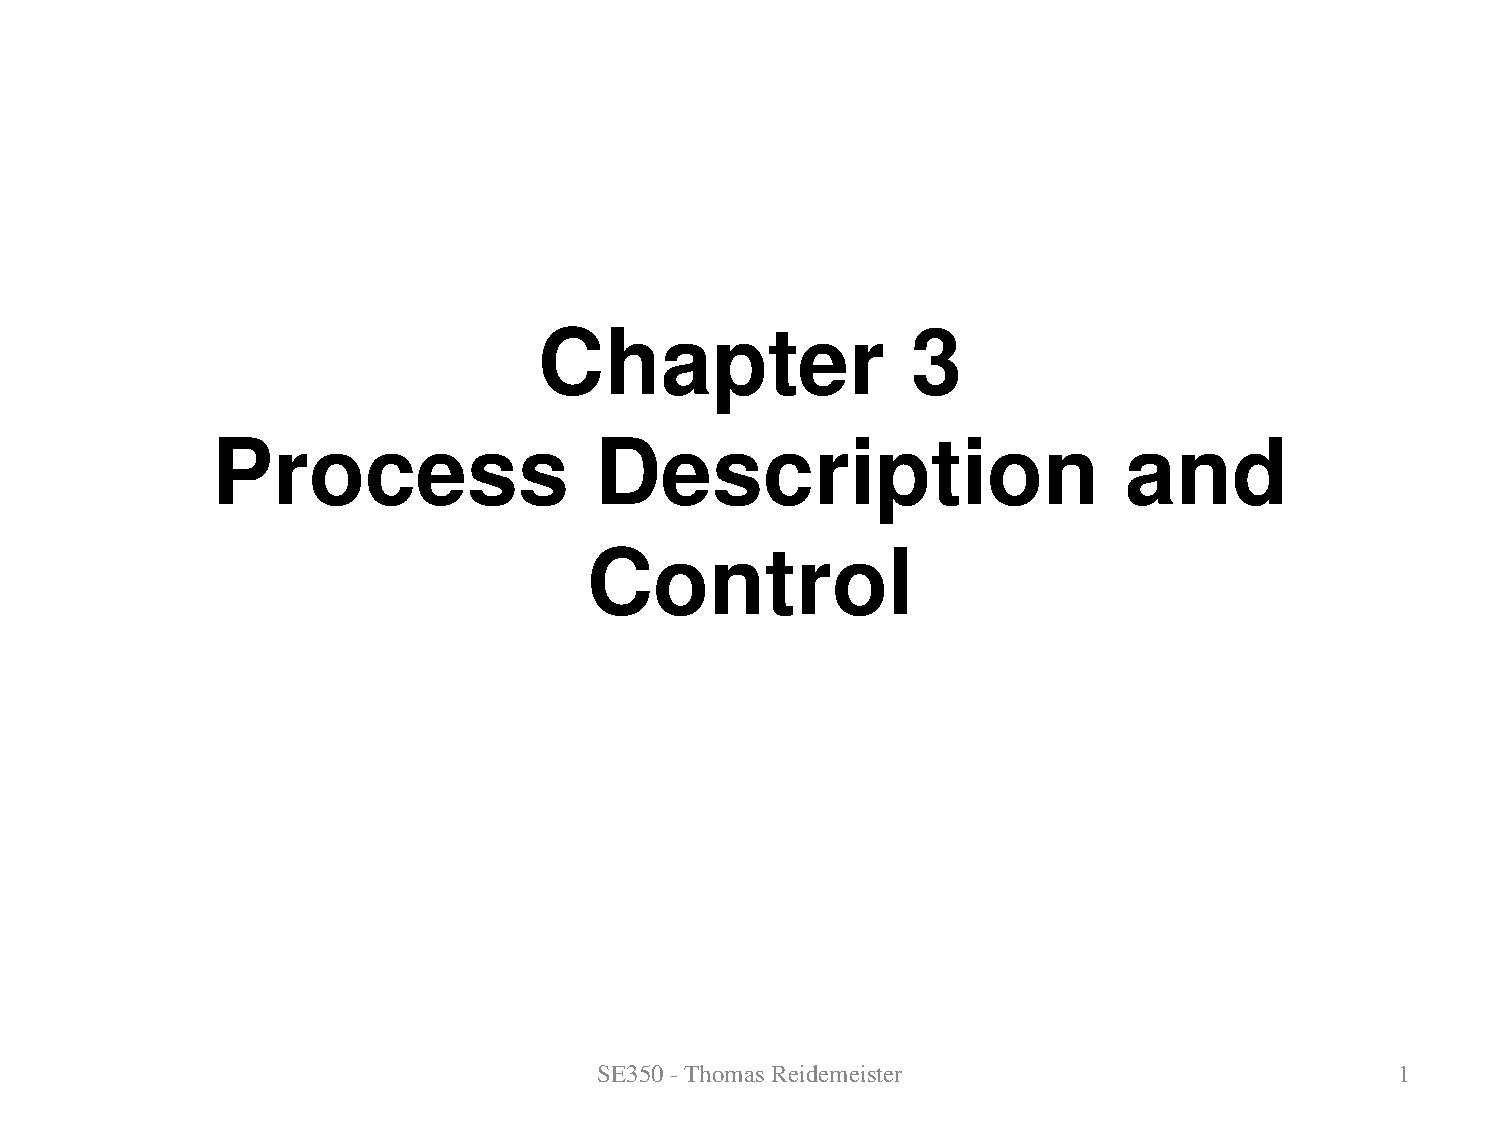
\includepdf[page=8]{03.pdf}
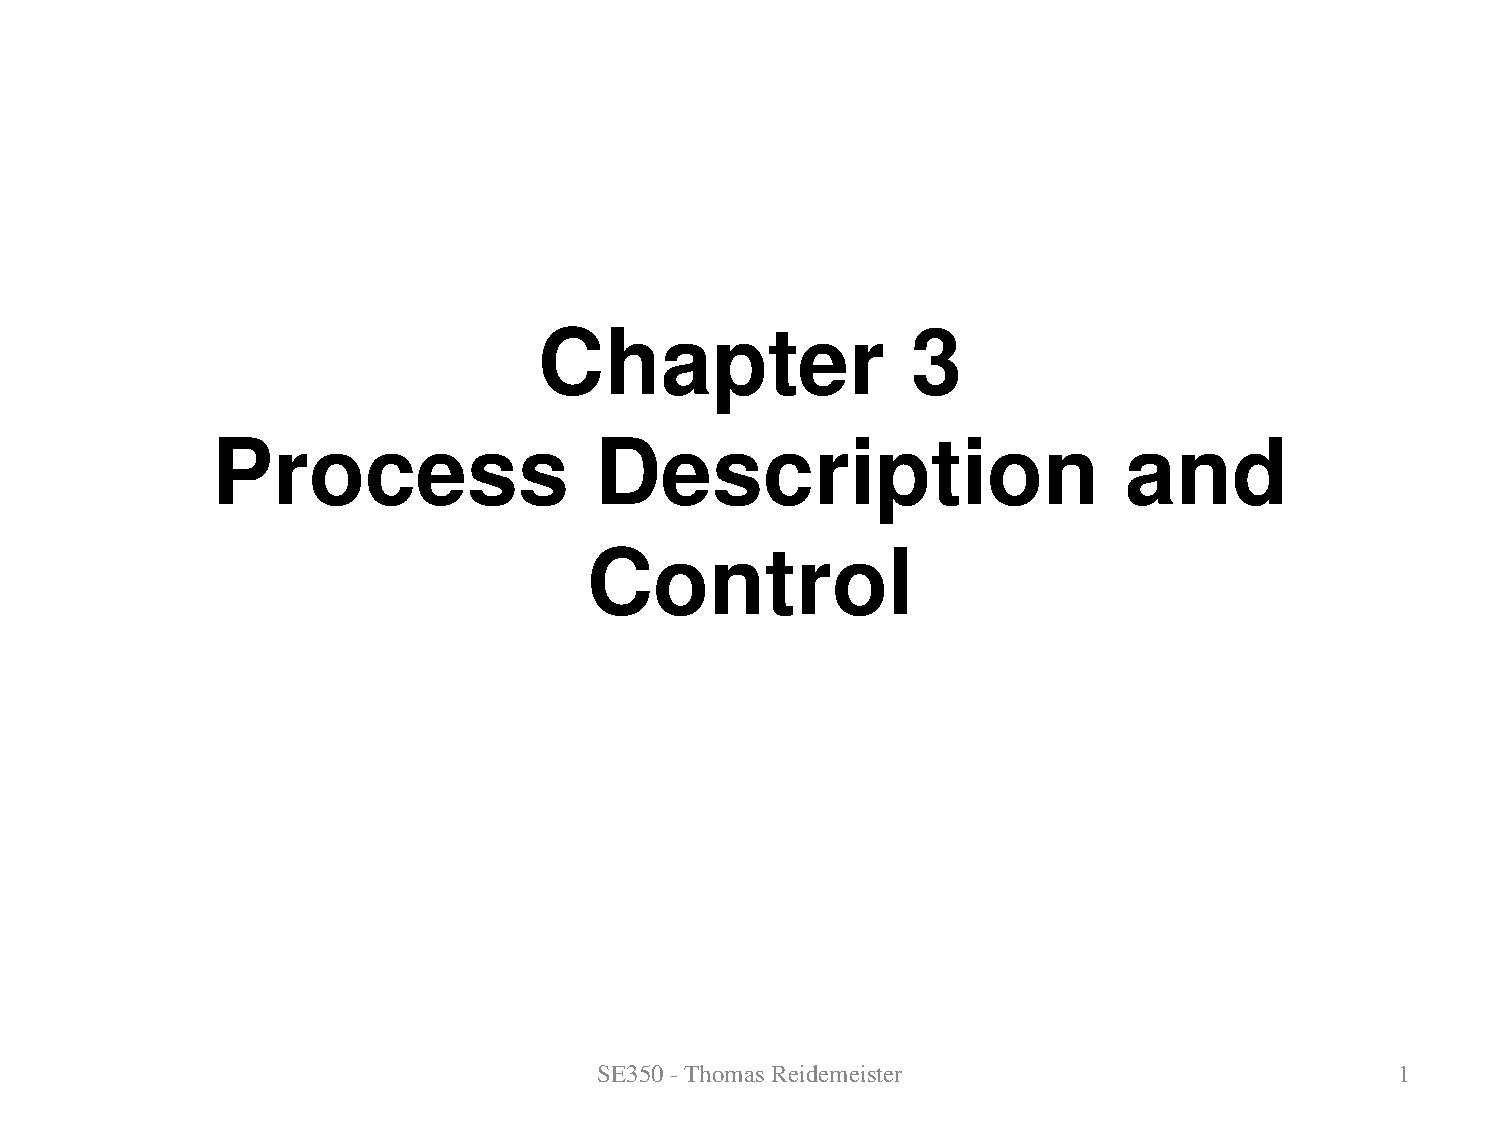
\includepdf[page=9]{03.pdf}
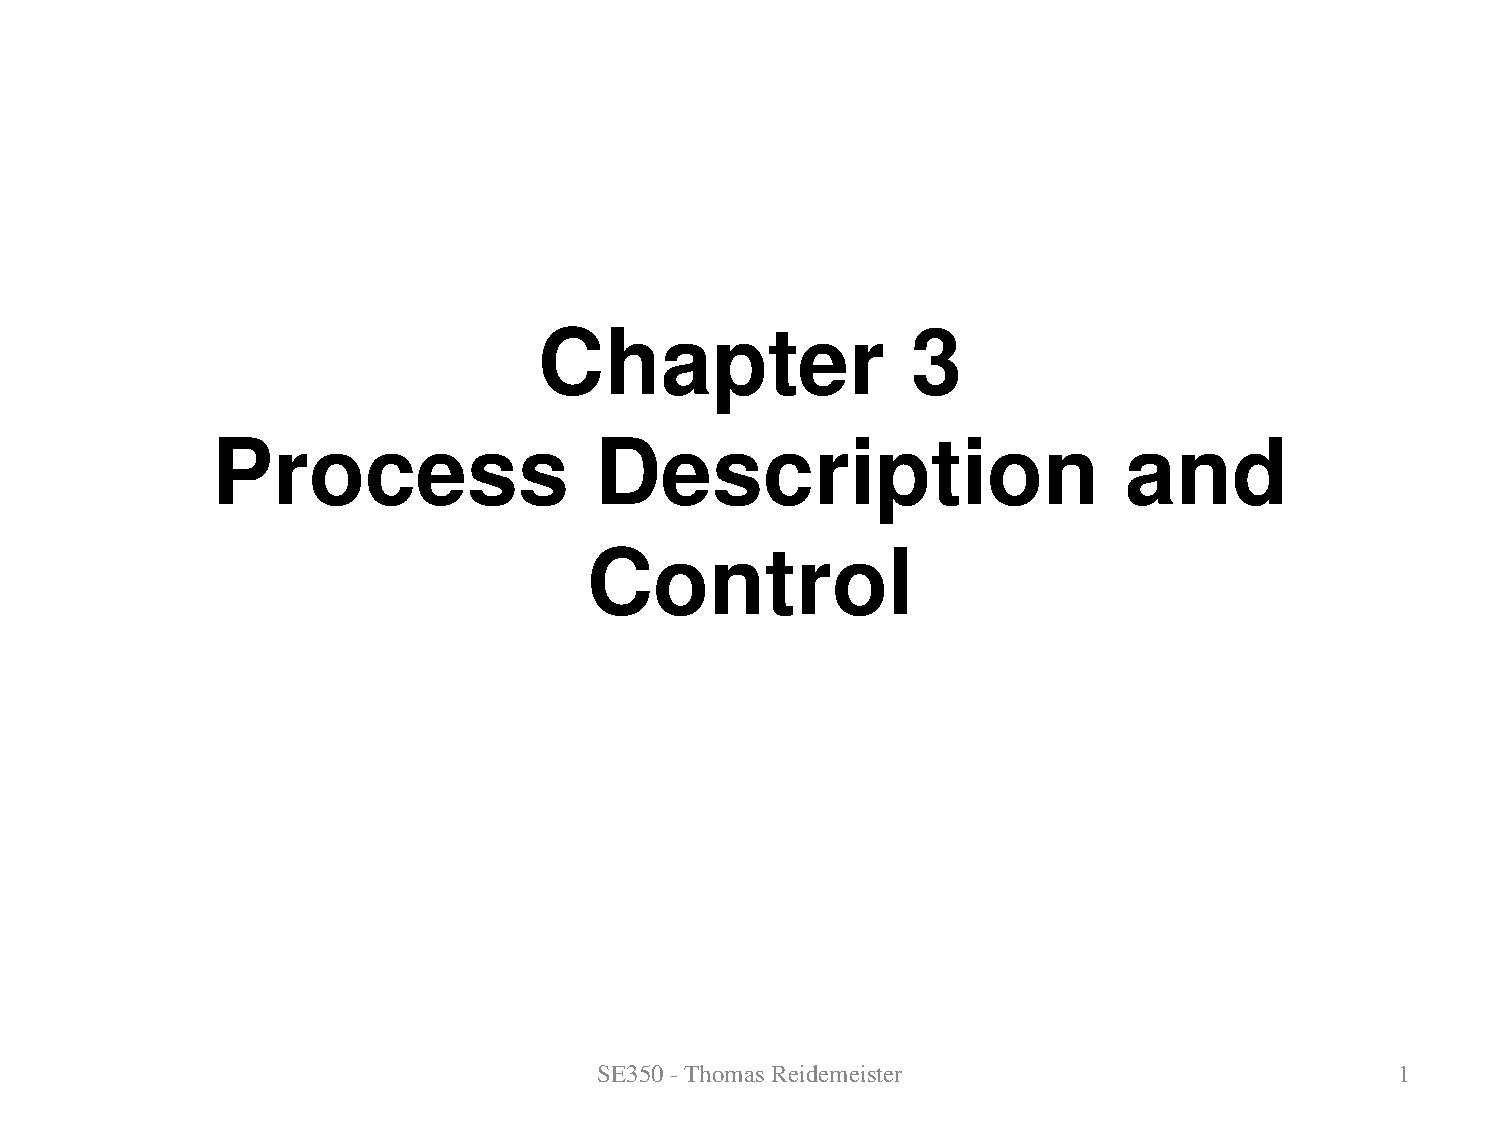
\includepdf[page=10]{03.pdf}
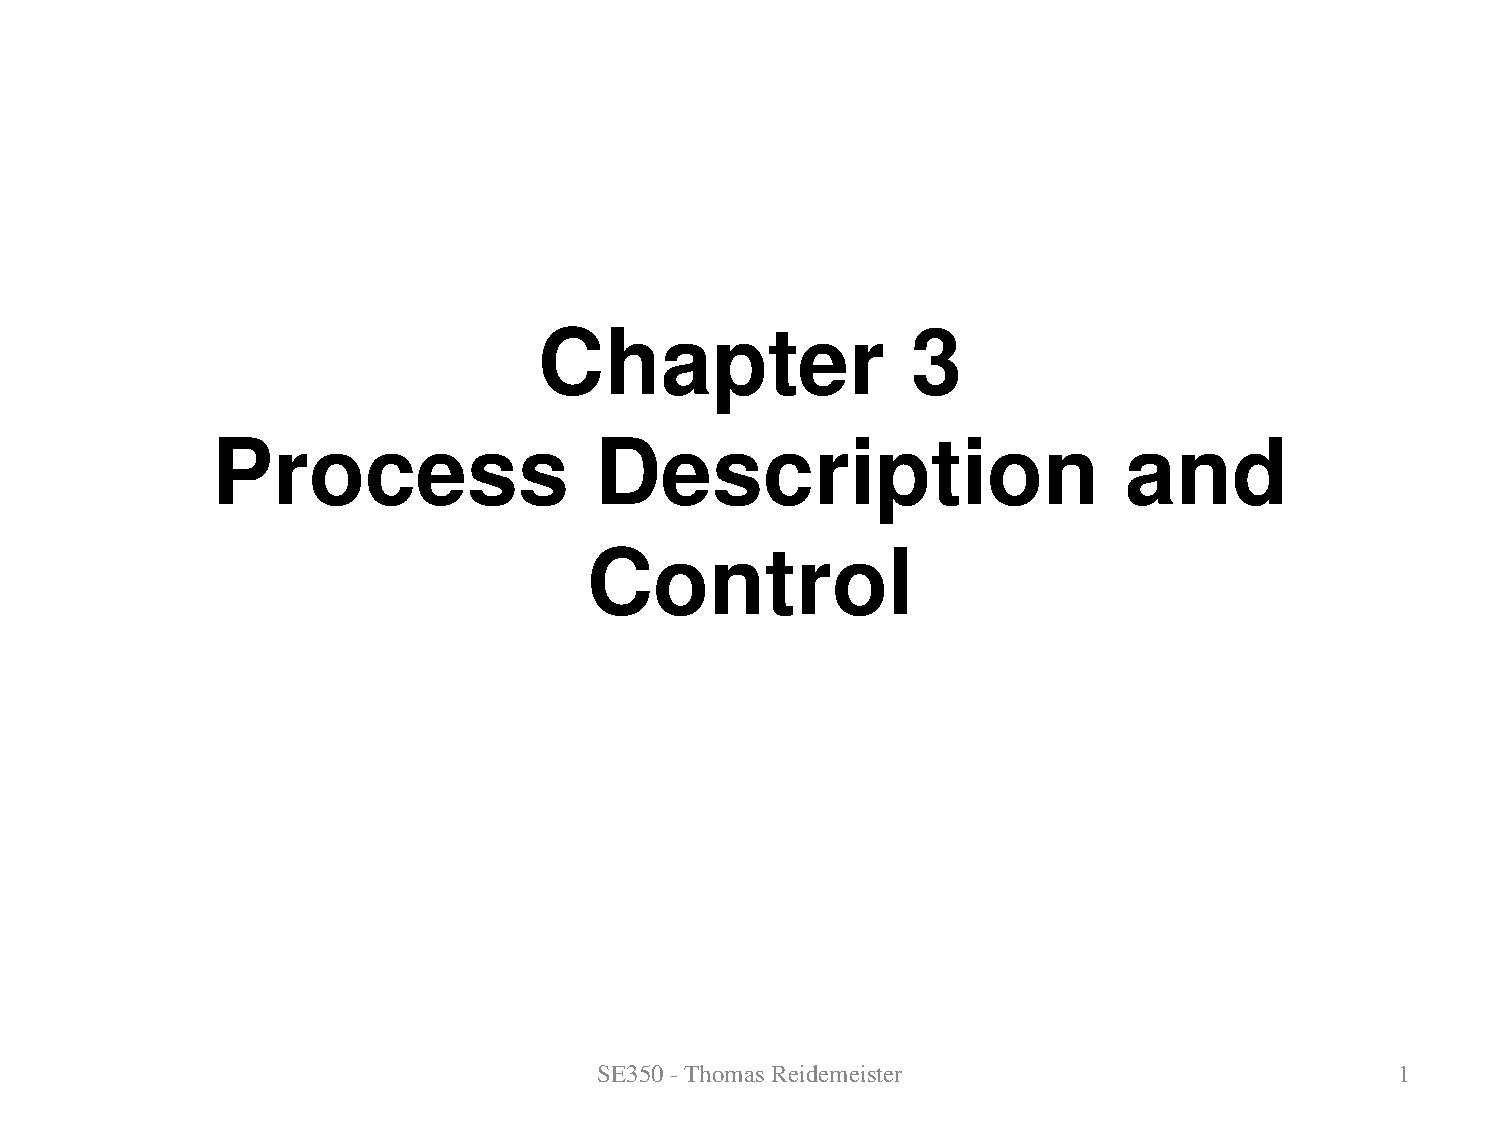
\includepdf[page=11]{03.pdf}
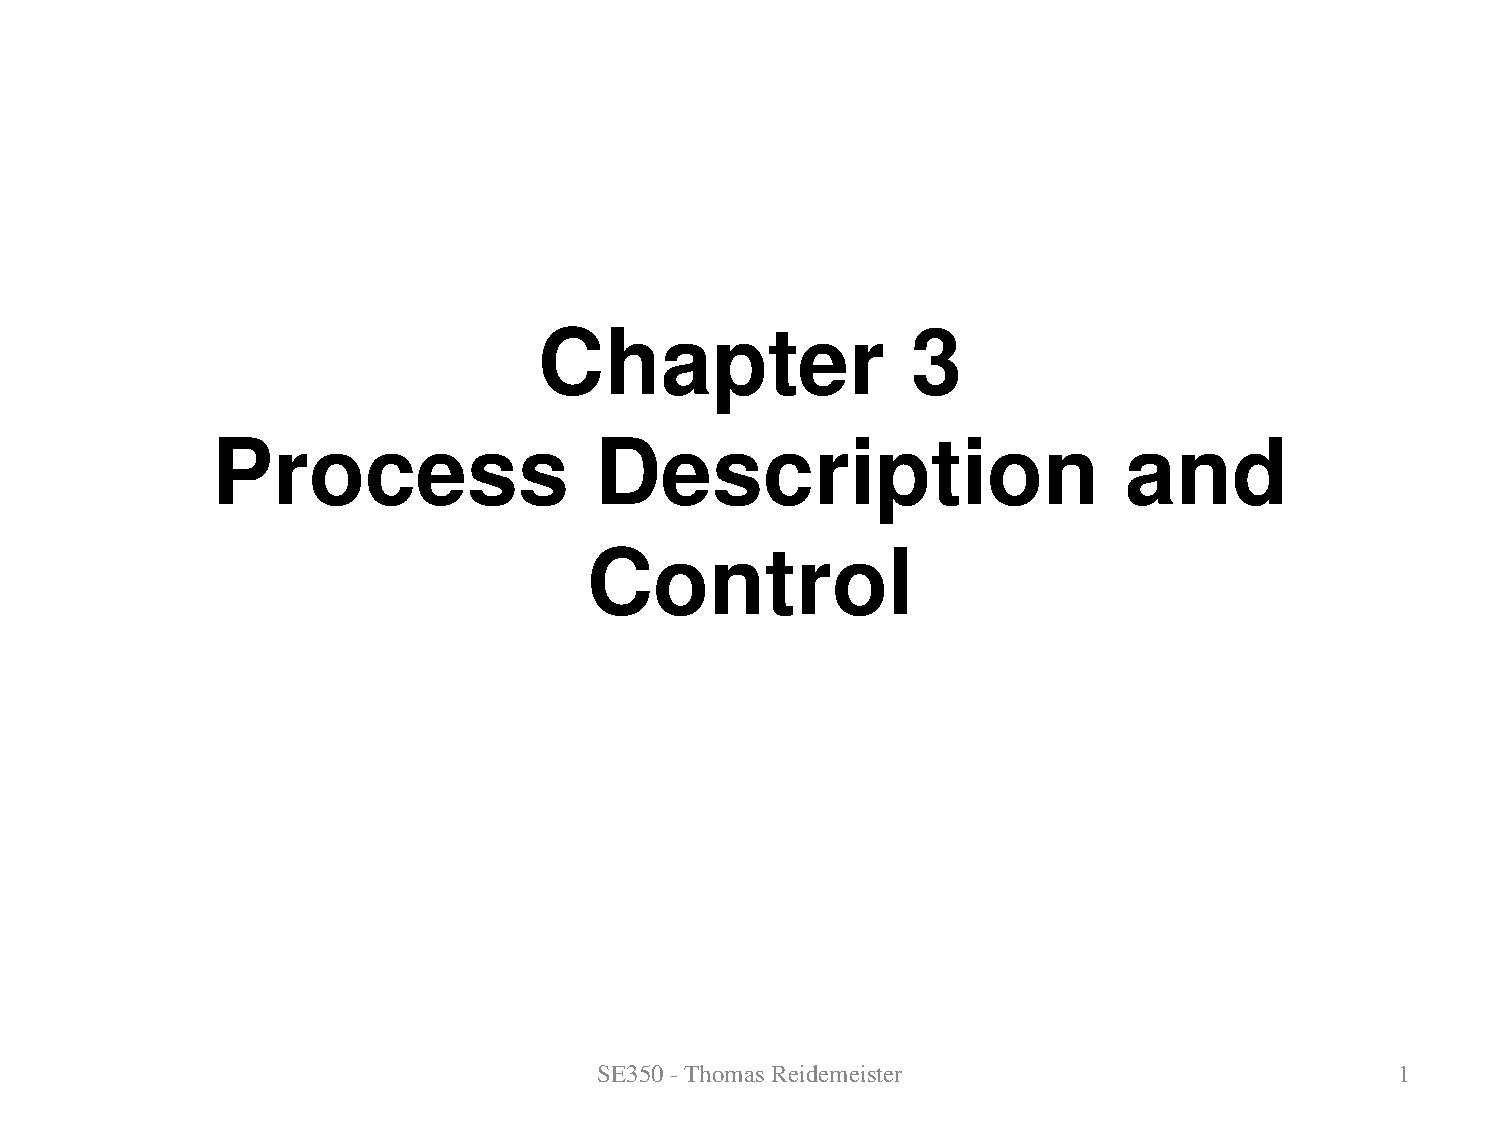
\includepdf[page=12]{03.pdf}
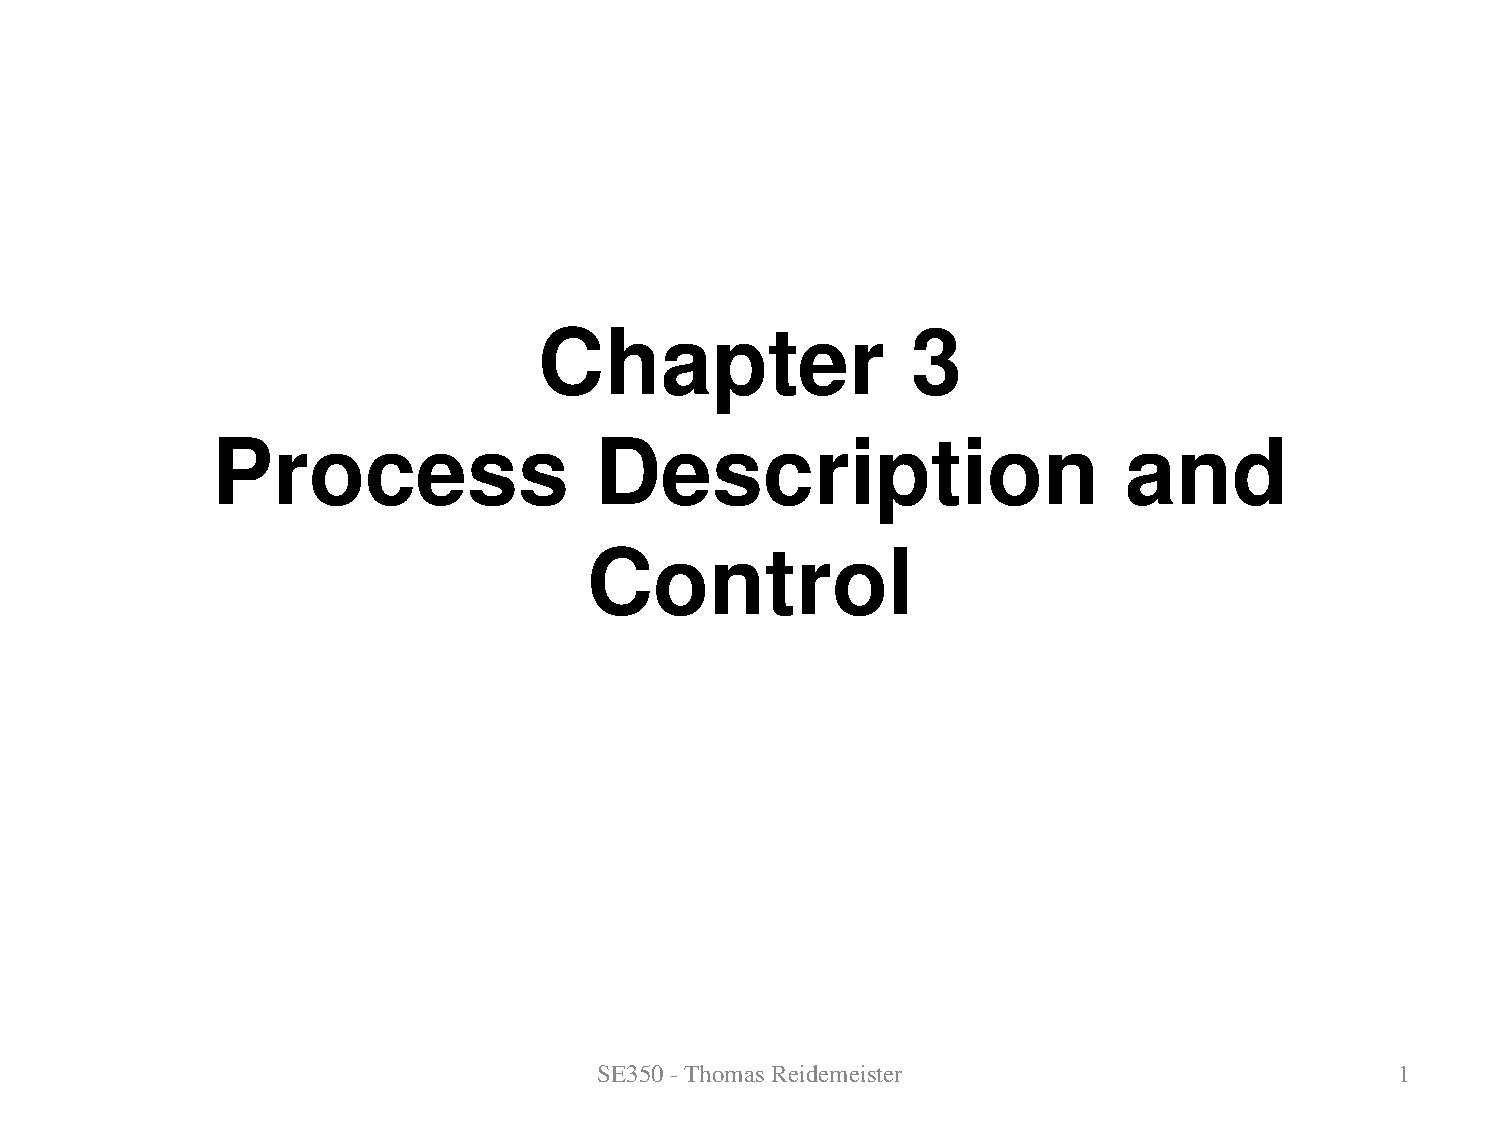
\includepdf[page=13]{03.pdf}
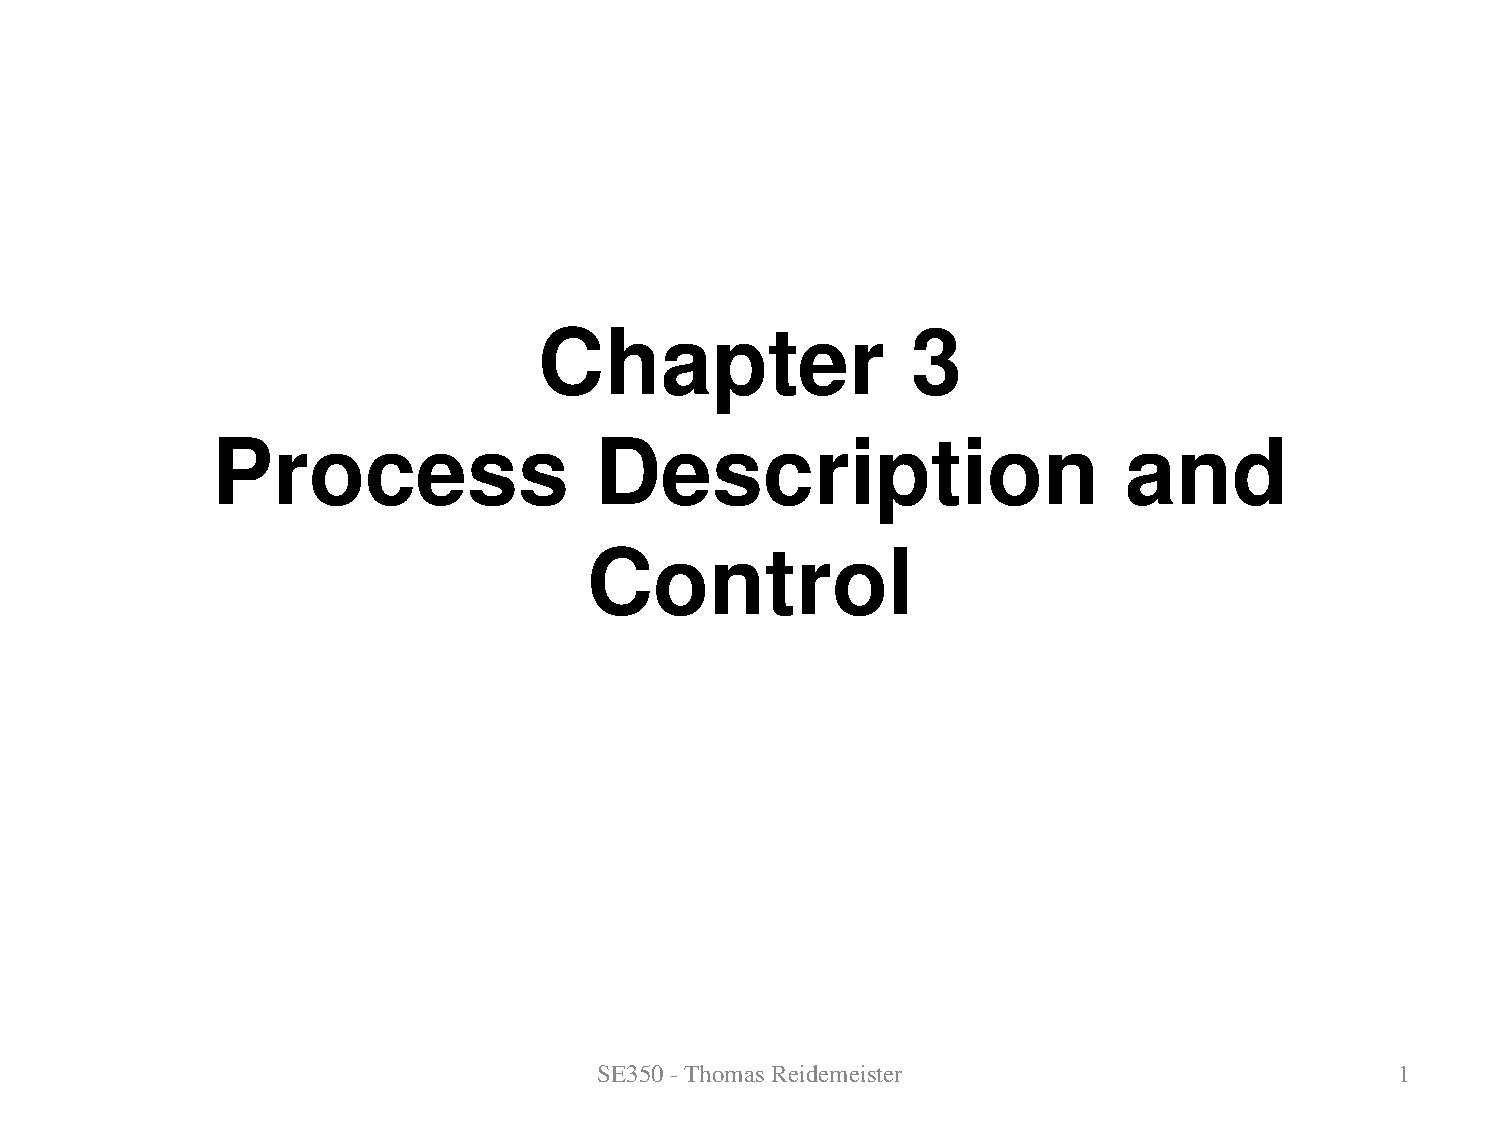
\includepdf[page=14]{03.pdf}
The trace by the OS is not necissary a sequence of instructions (that is how it looks to the process though)
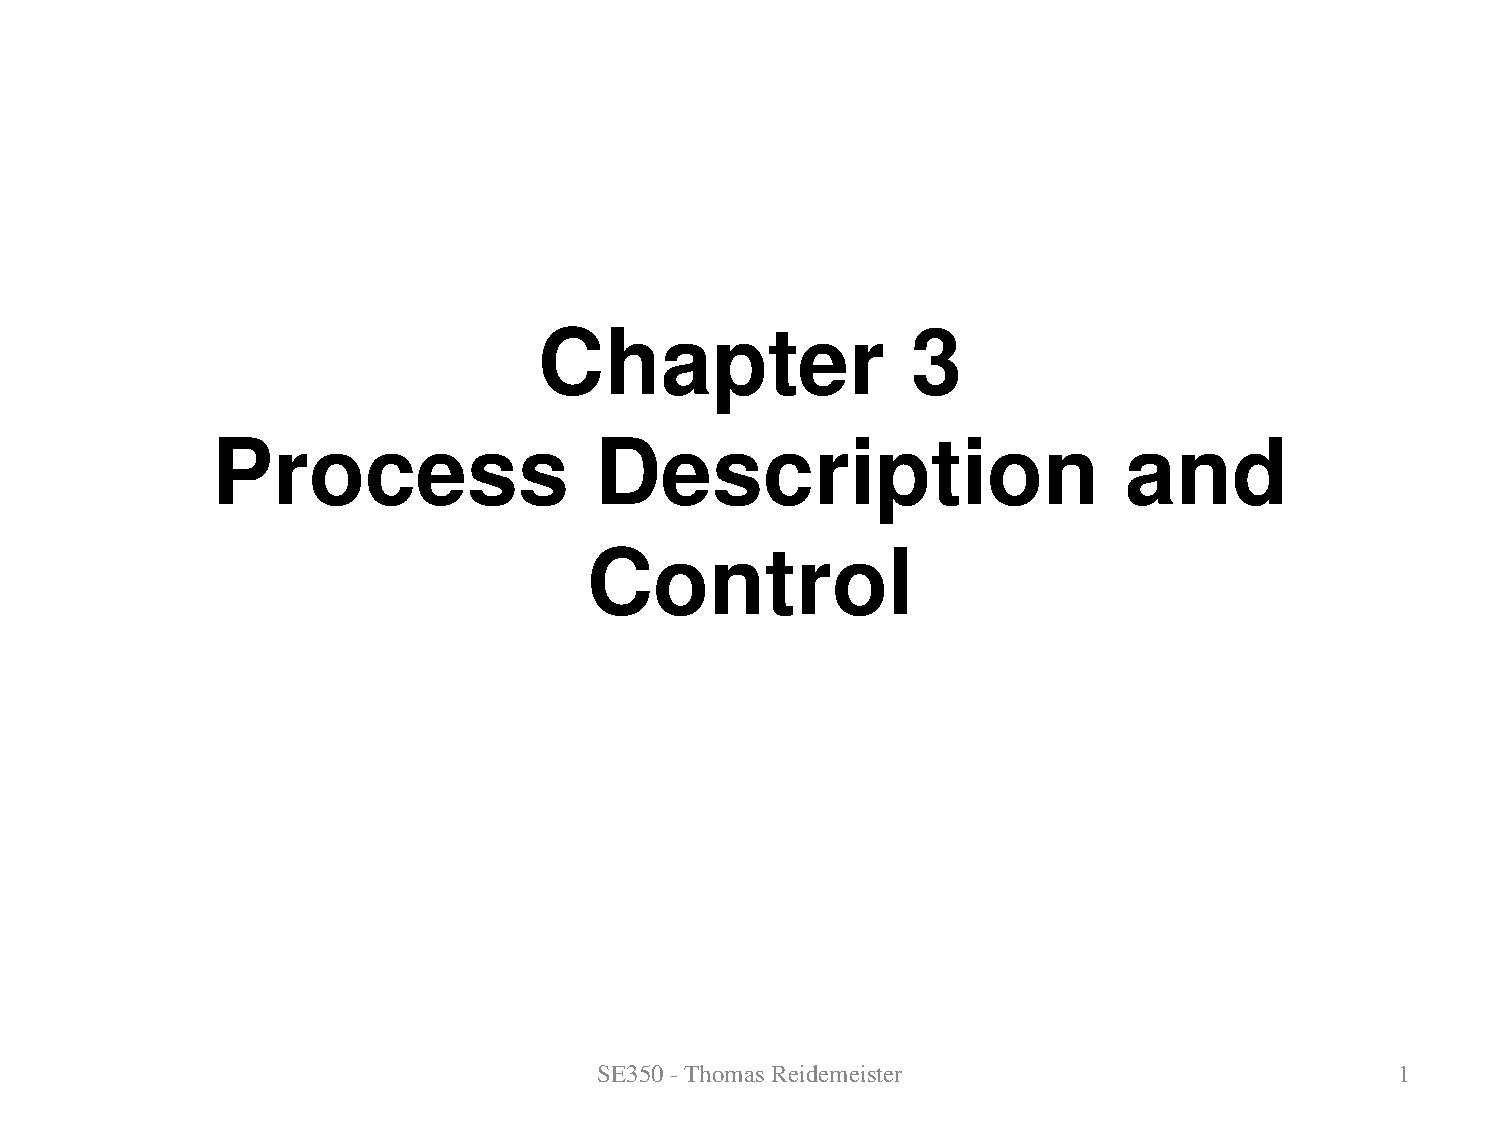
\includepdf[page=15]{03.pdf}
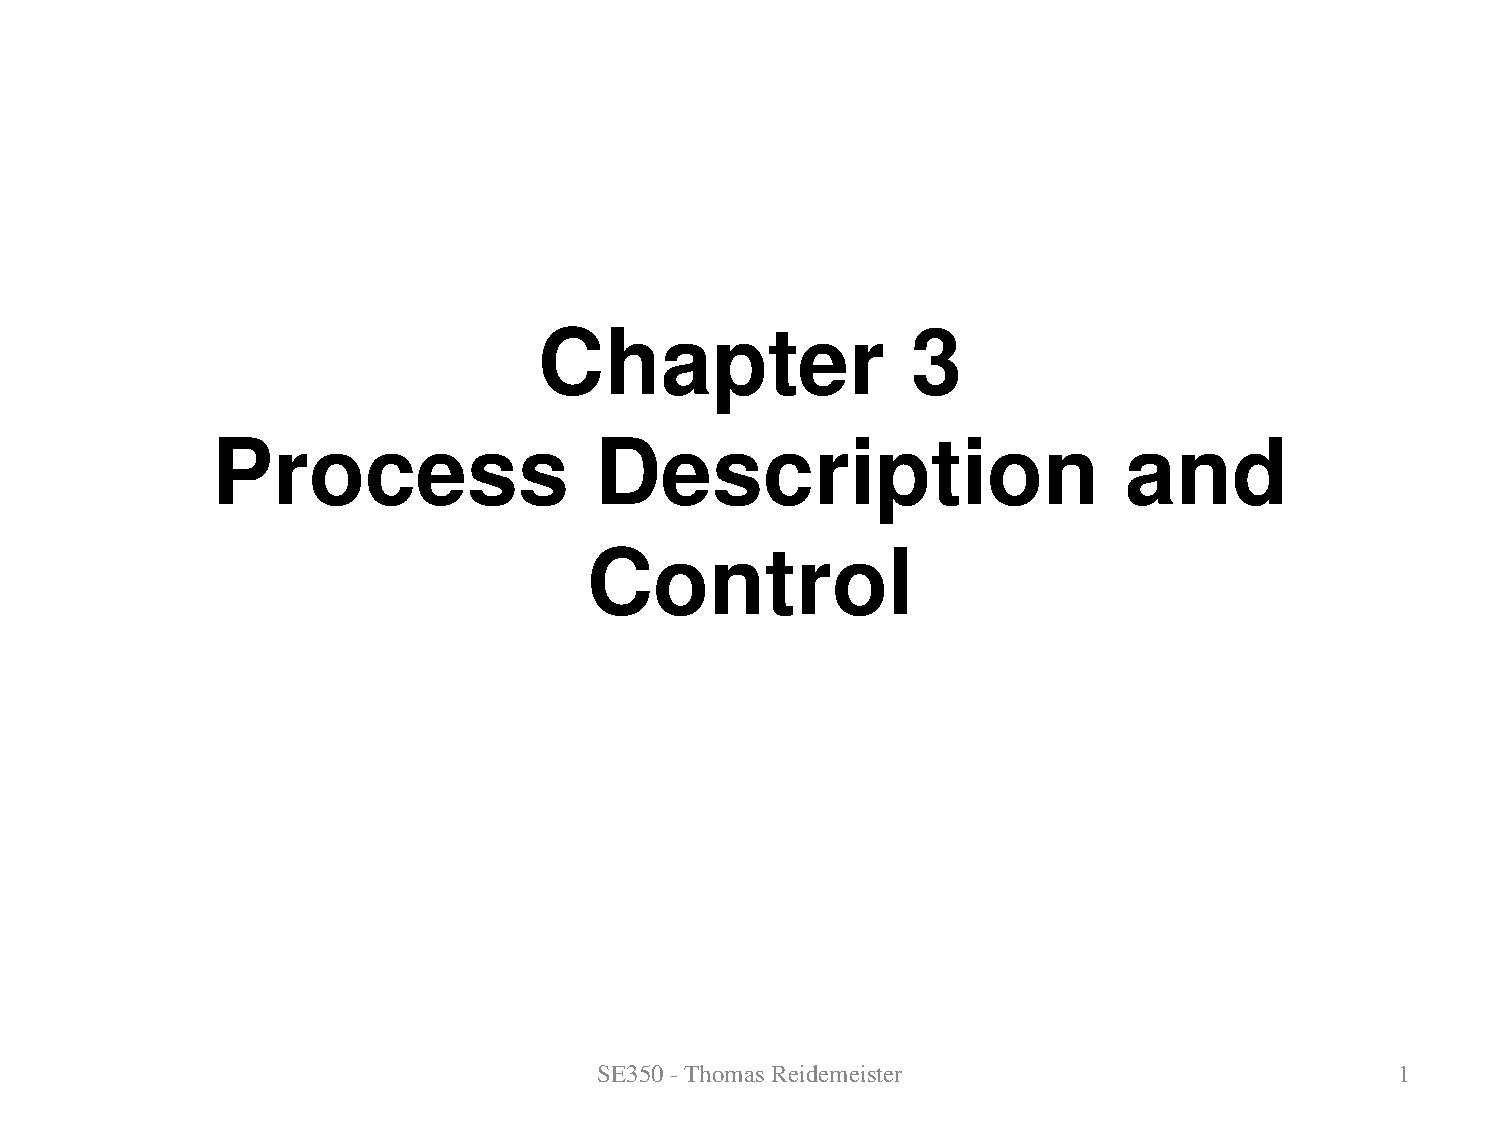
\includepdf[page=16]{03.pdf}
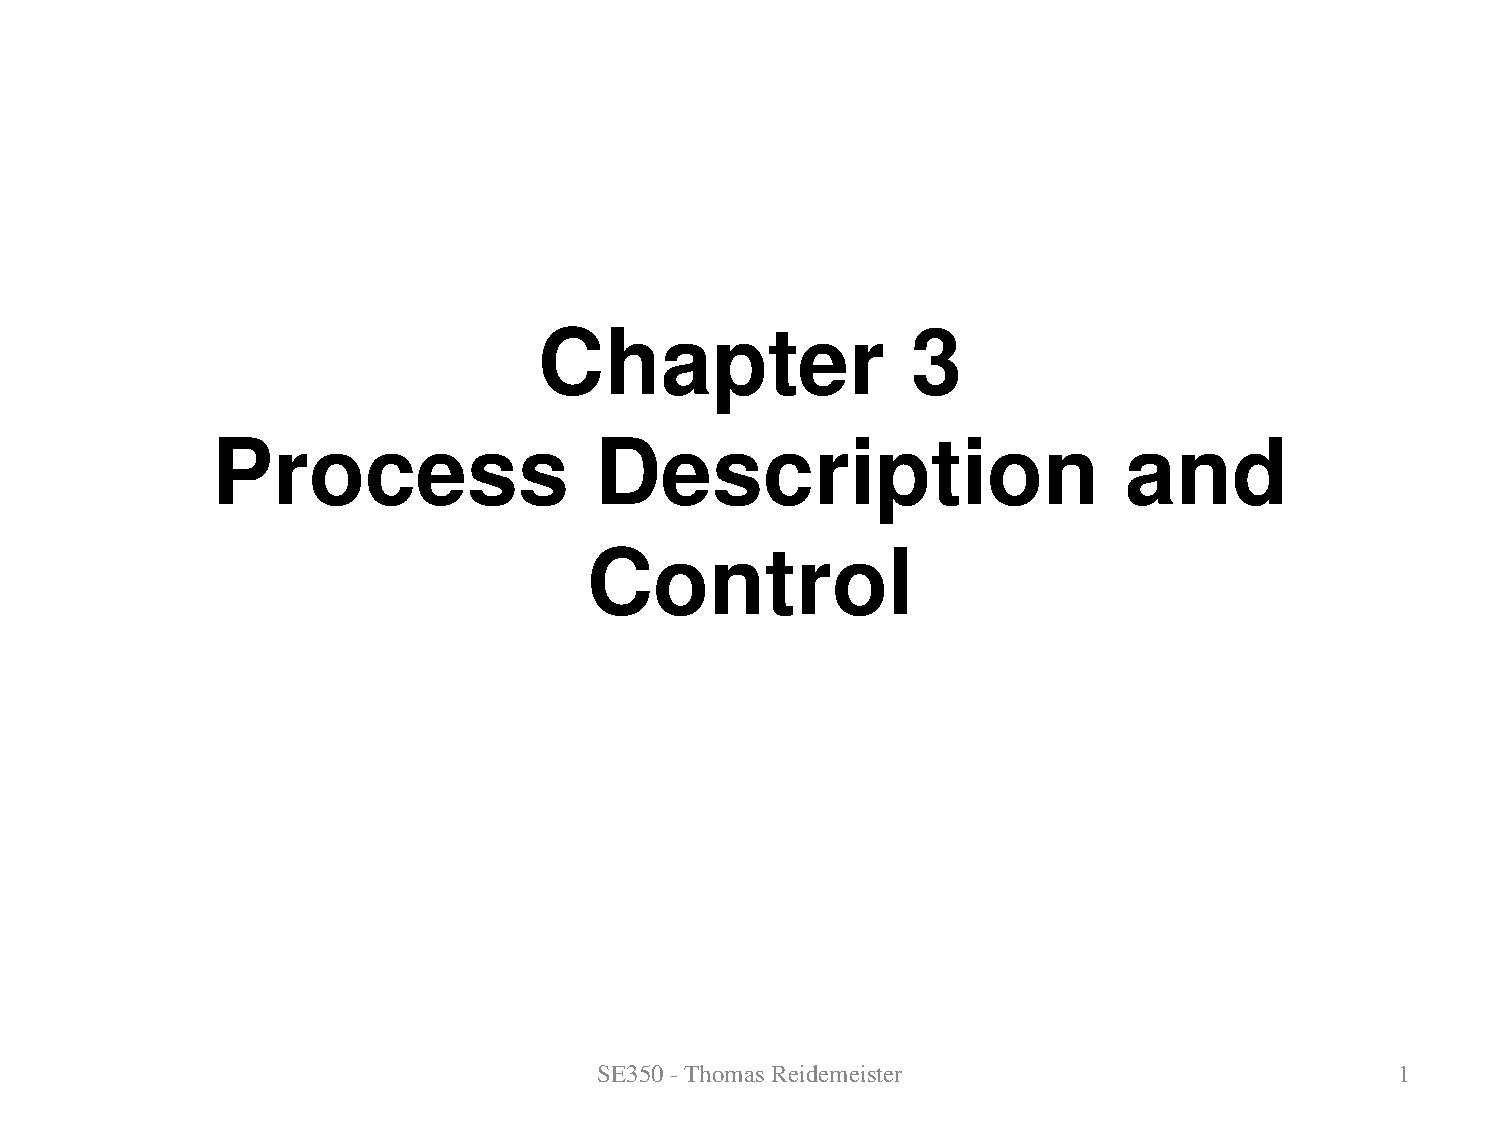
\includepdf[page=17]{03.pdf}
We can see here that to the OS a trace is not sequential because there are breaks where we make IO requests and have timeouts. We dont actually have processes executing in parallel, but the processor just jumps between them alot.
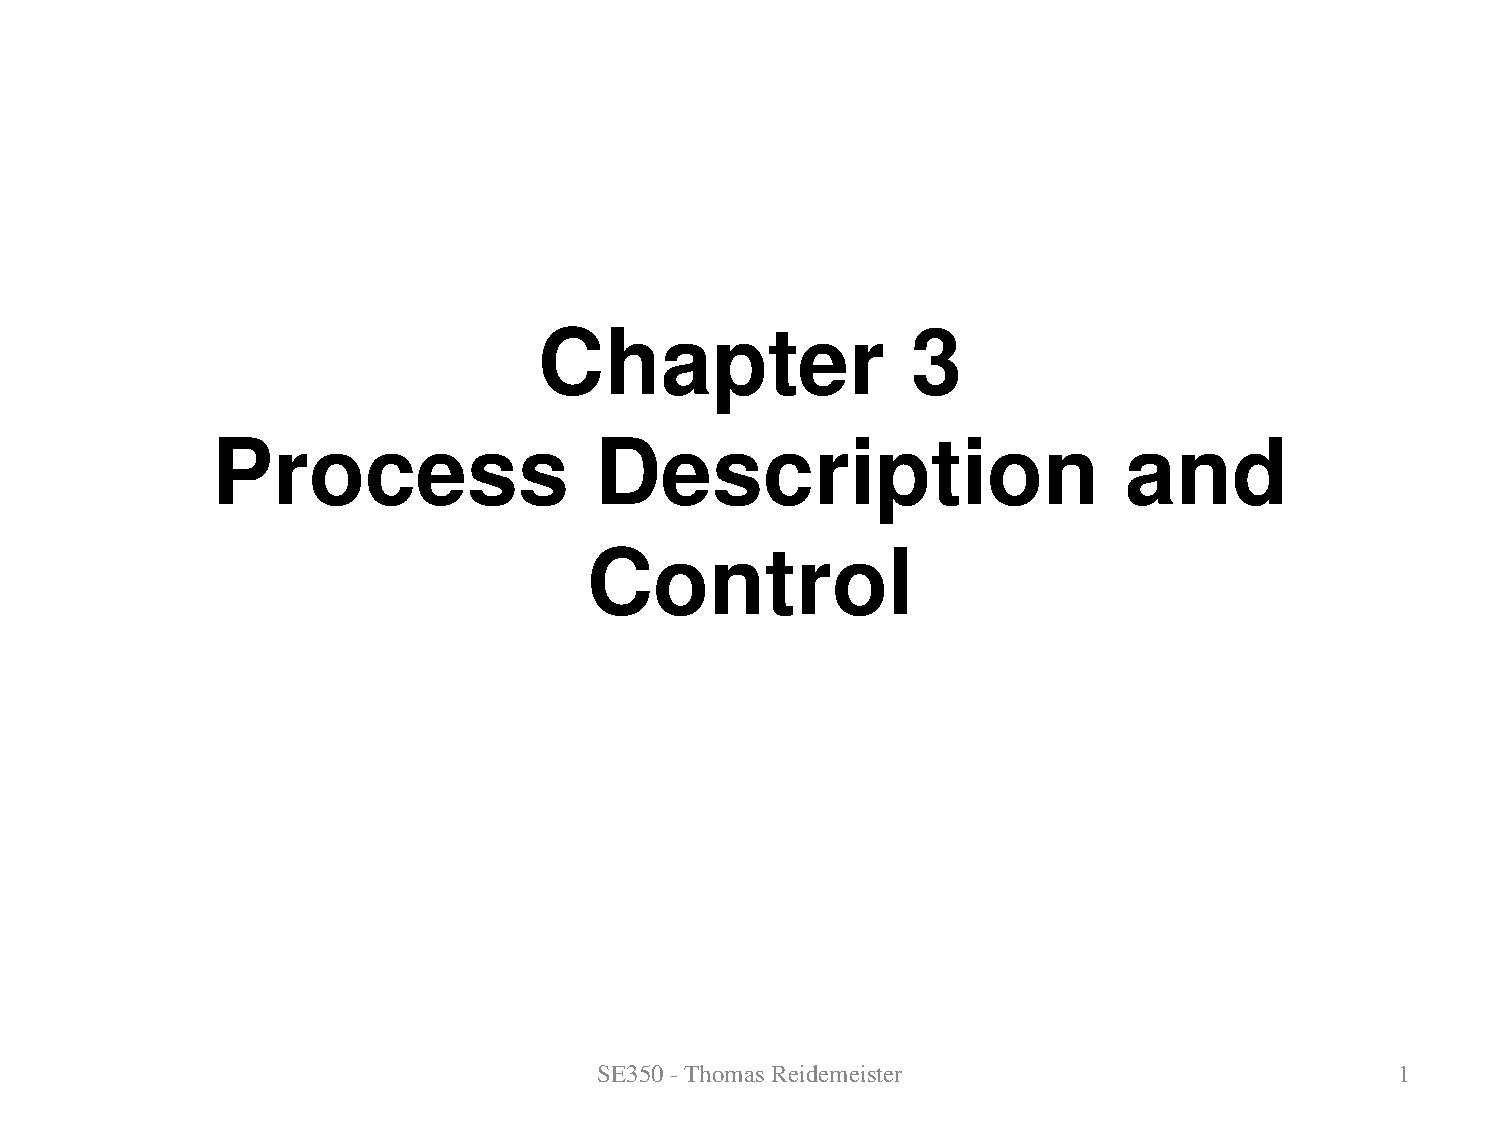
\includepdf[page=18]{03.pdf}
This is a very simple model to hold the state of the process. Either the proccess is running or not. The process just gets looped between those states every time interrupts happen. We have a pointer to the currently running process (remember that process have their state saved on them). When an interrupt happens the dispatcher grabs the next processor that is not running to resume work on that.
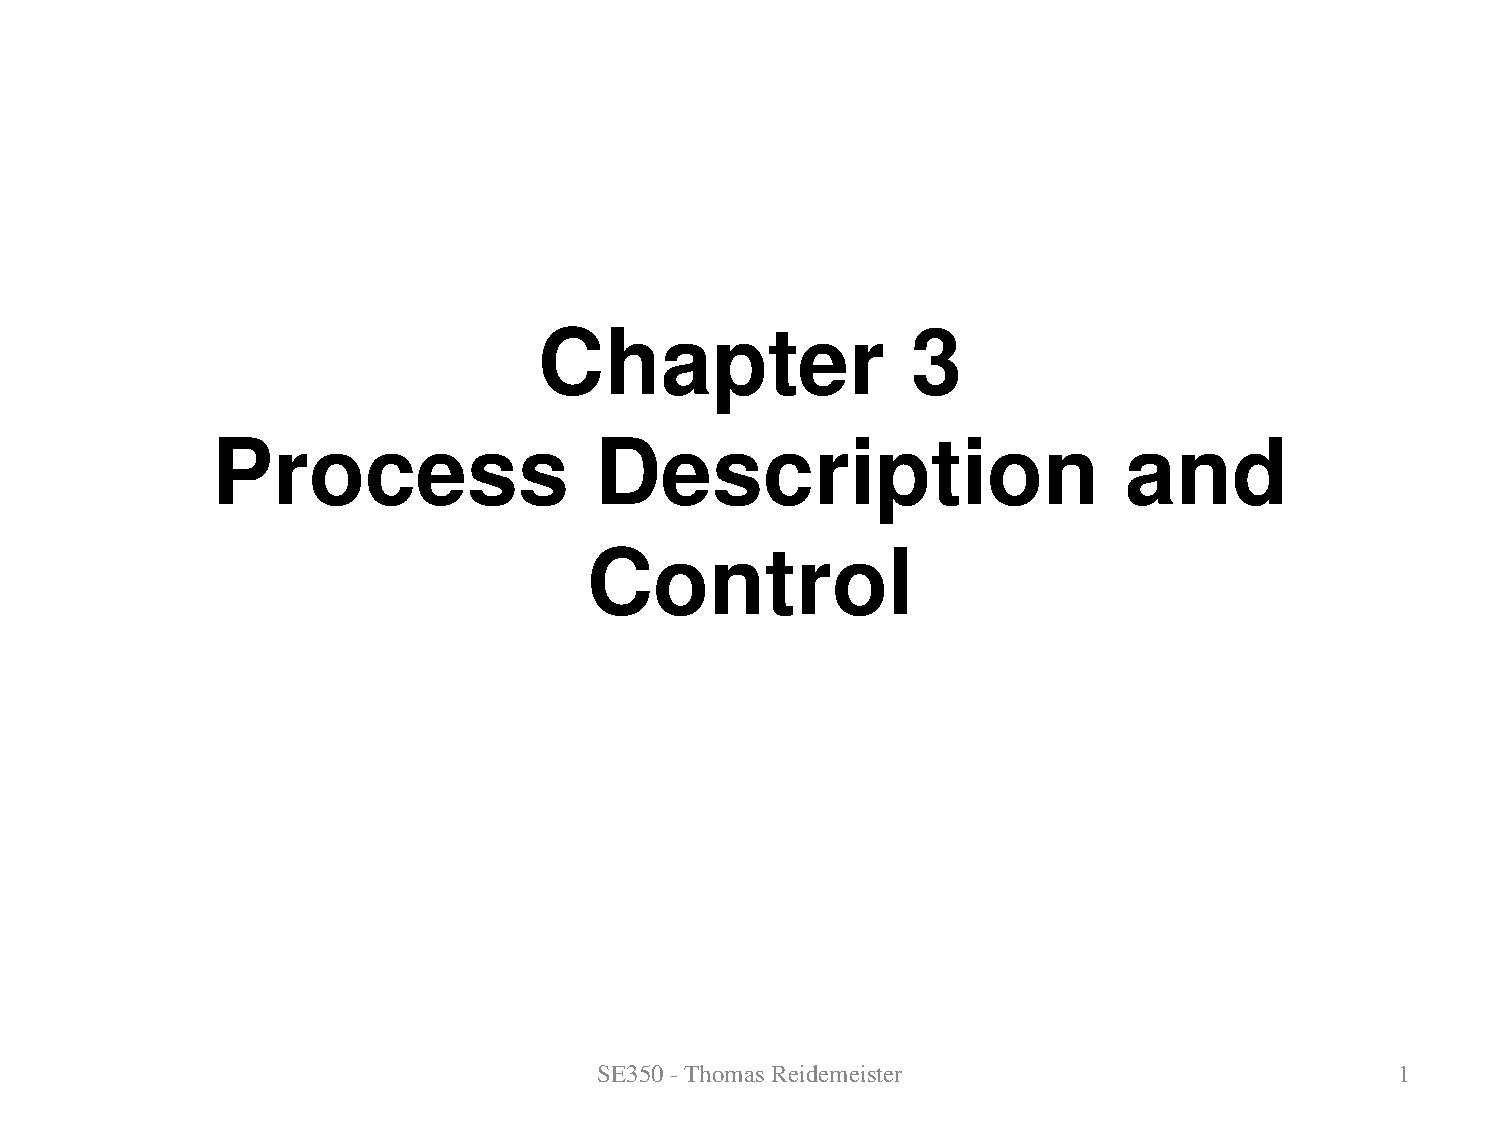
\includepdf[page=19]{03.pdf}
When a process is not running on the cpu we put in on the queue and switch its state to running and pop it off when the cpu is free
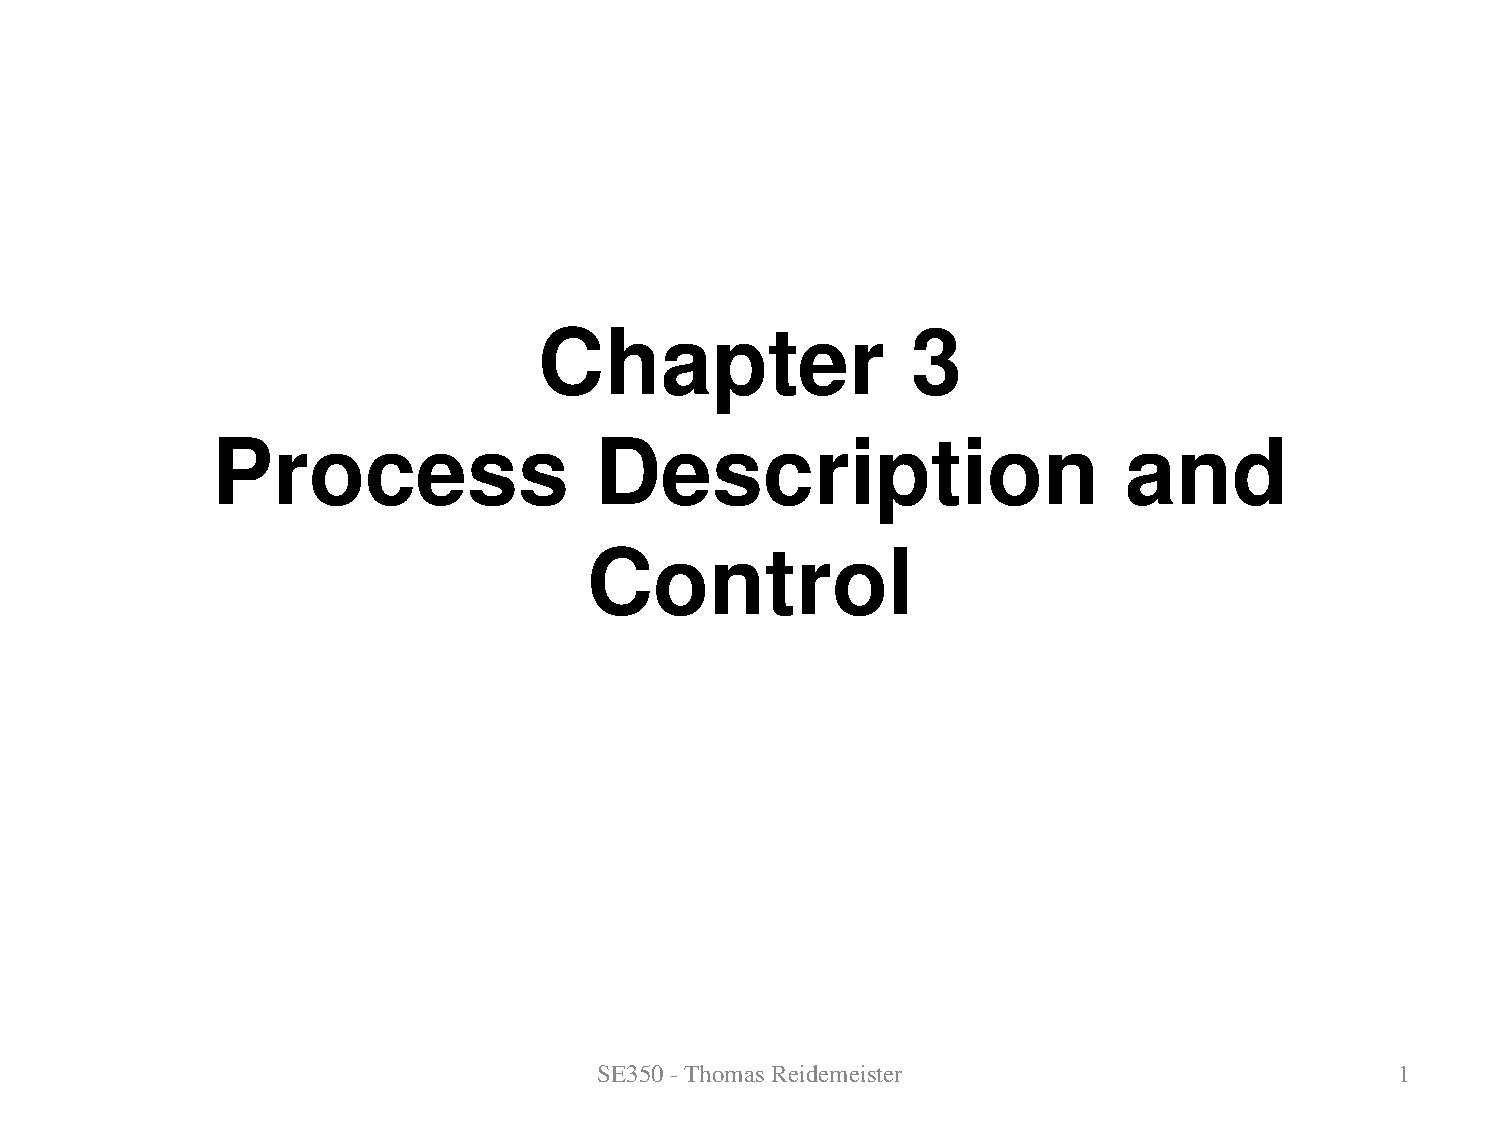
\includepdf[page=20]{03.pdf}
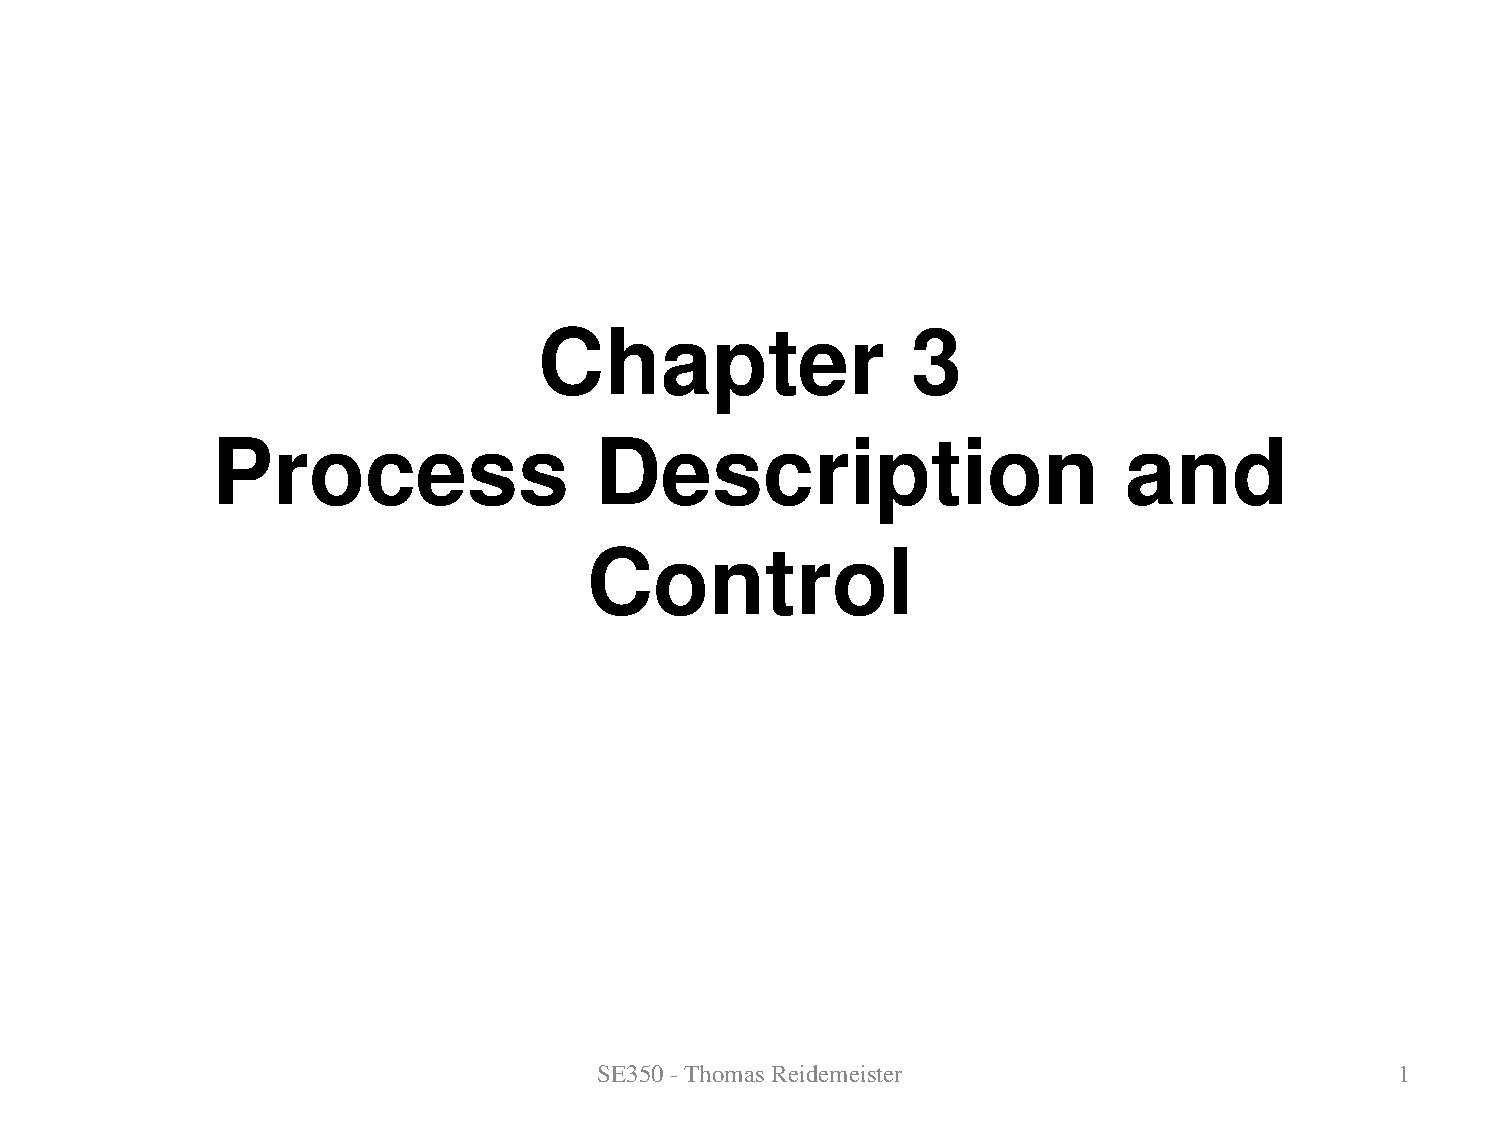
\includepdf[page=21]{03.pdf}
A core dump is the current execution context at the process termination.
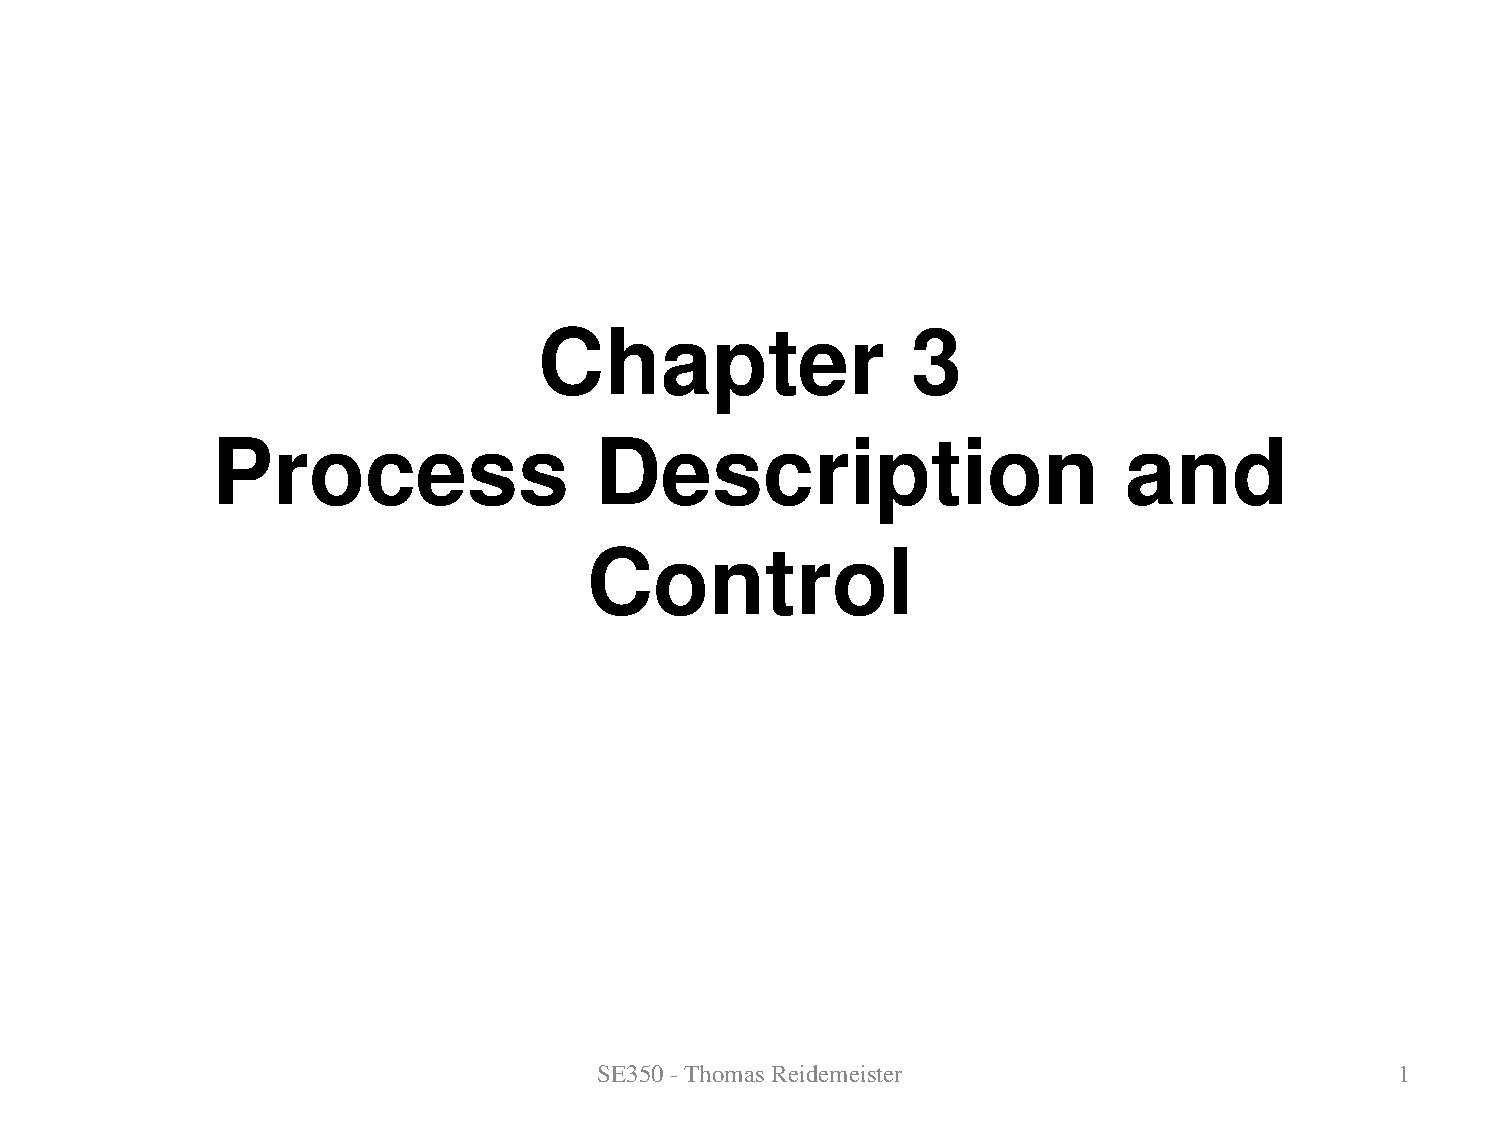
\includepdf[page=22]{03.pdf}
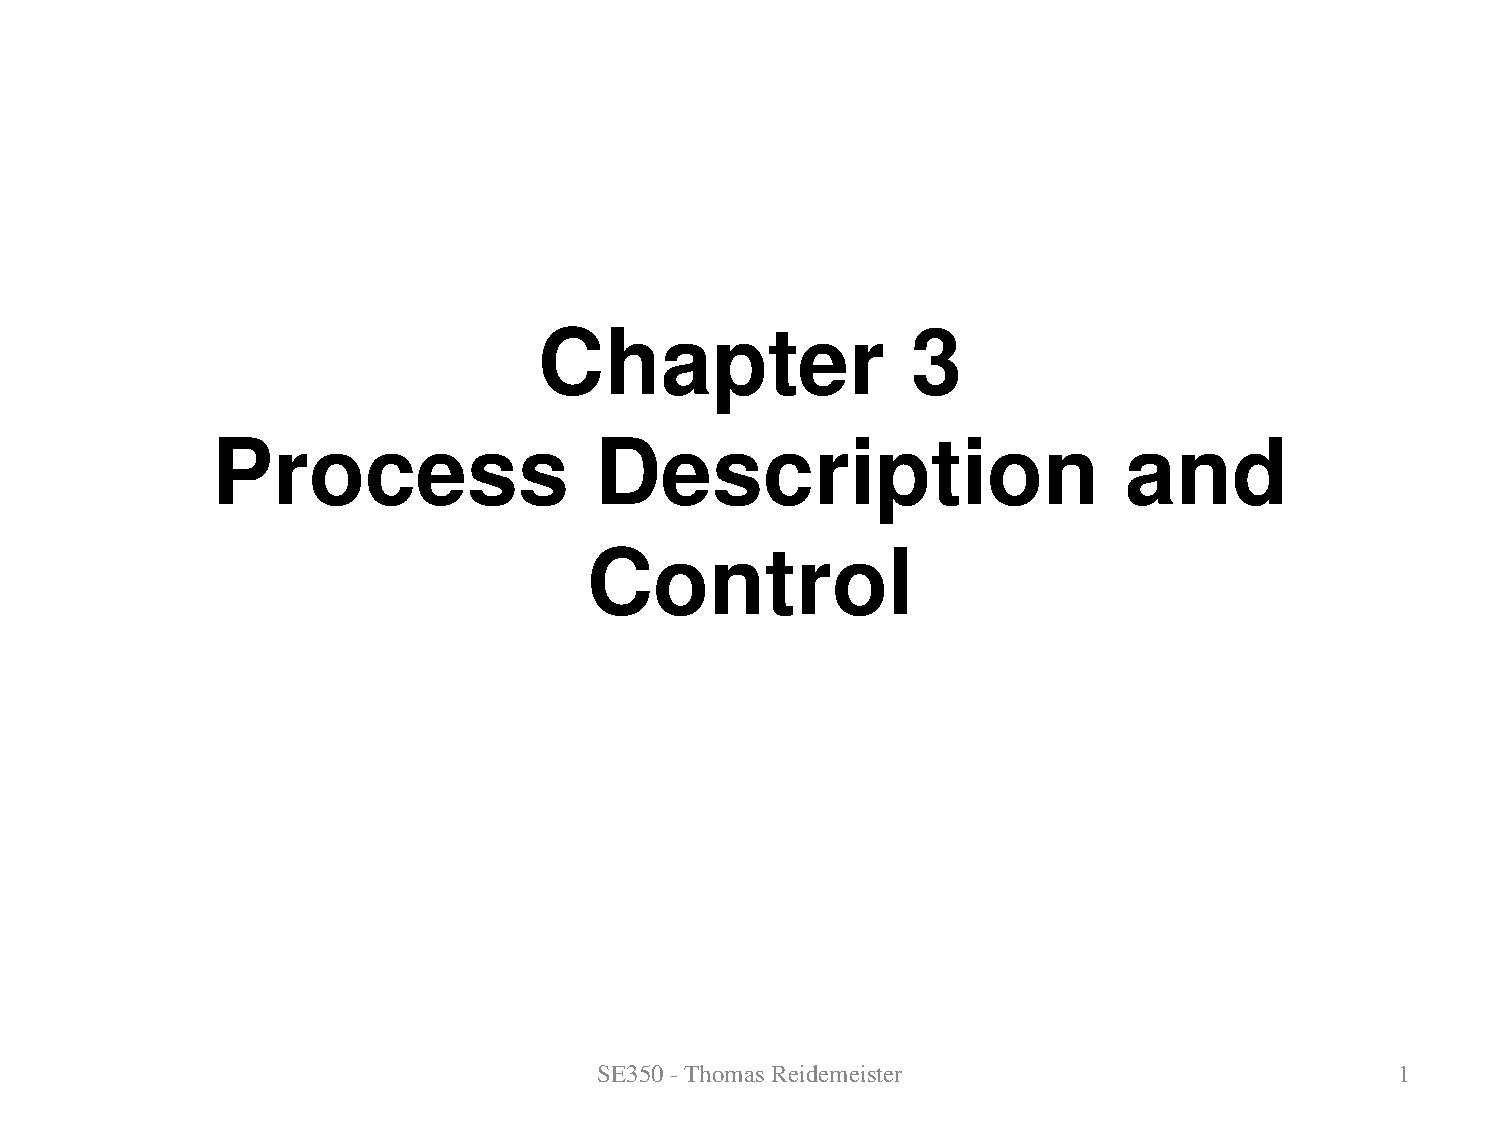
\includepdf[page=23]{03.pdf}
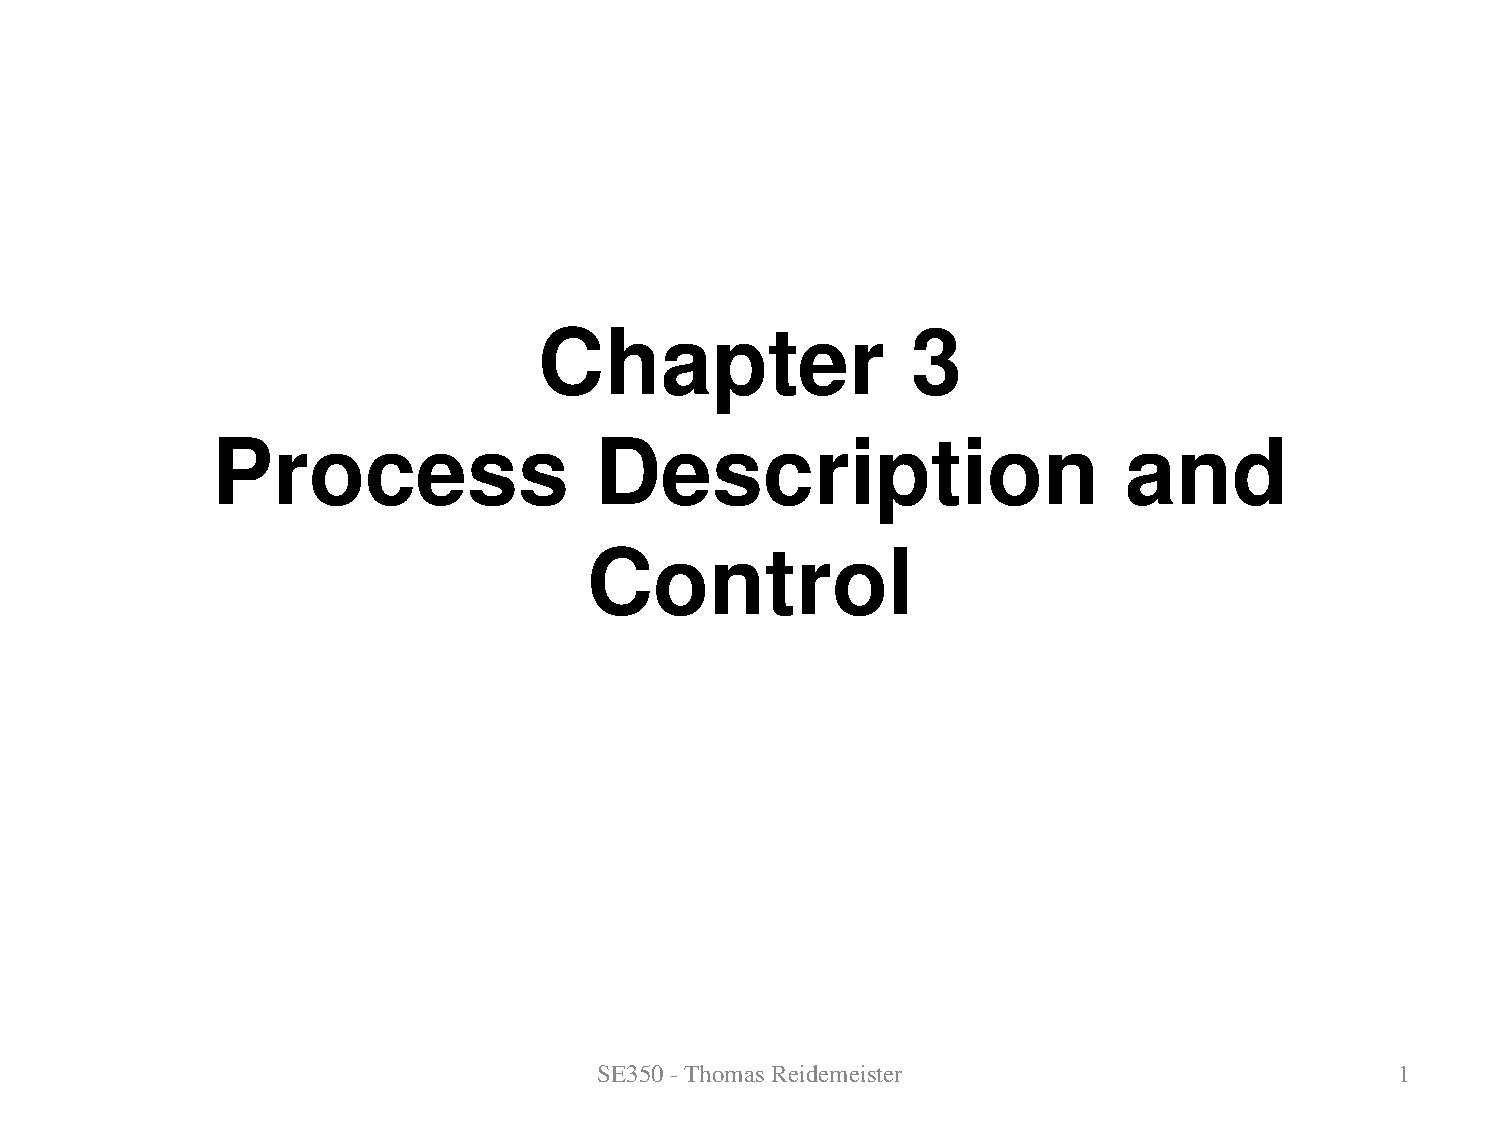
\includepdf[page=24]{03.pdf}
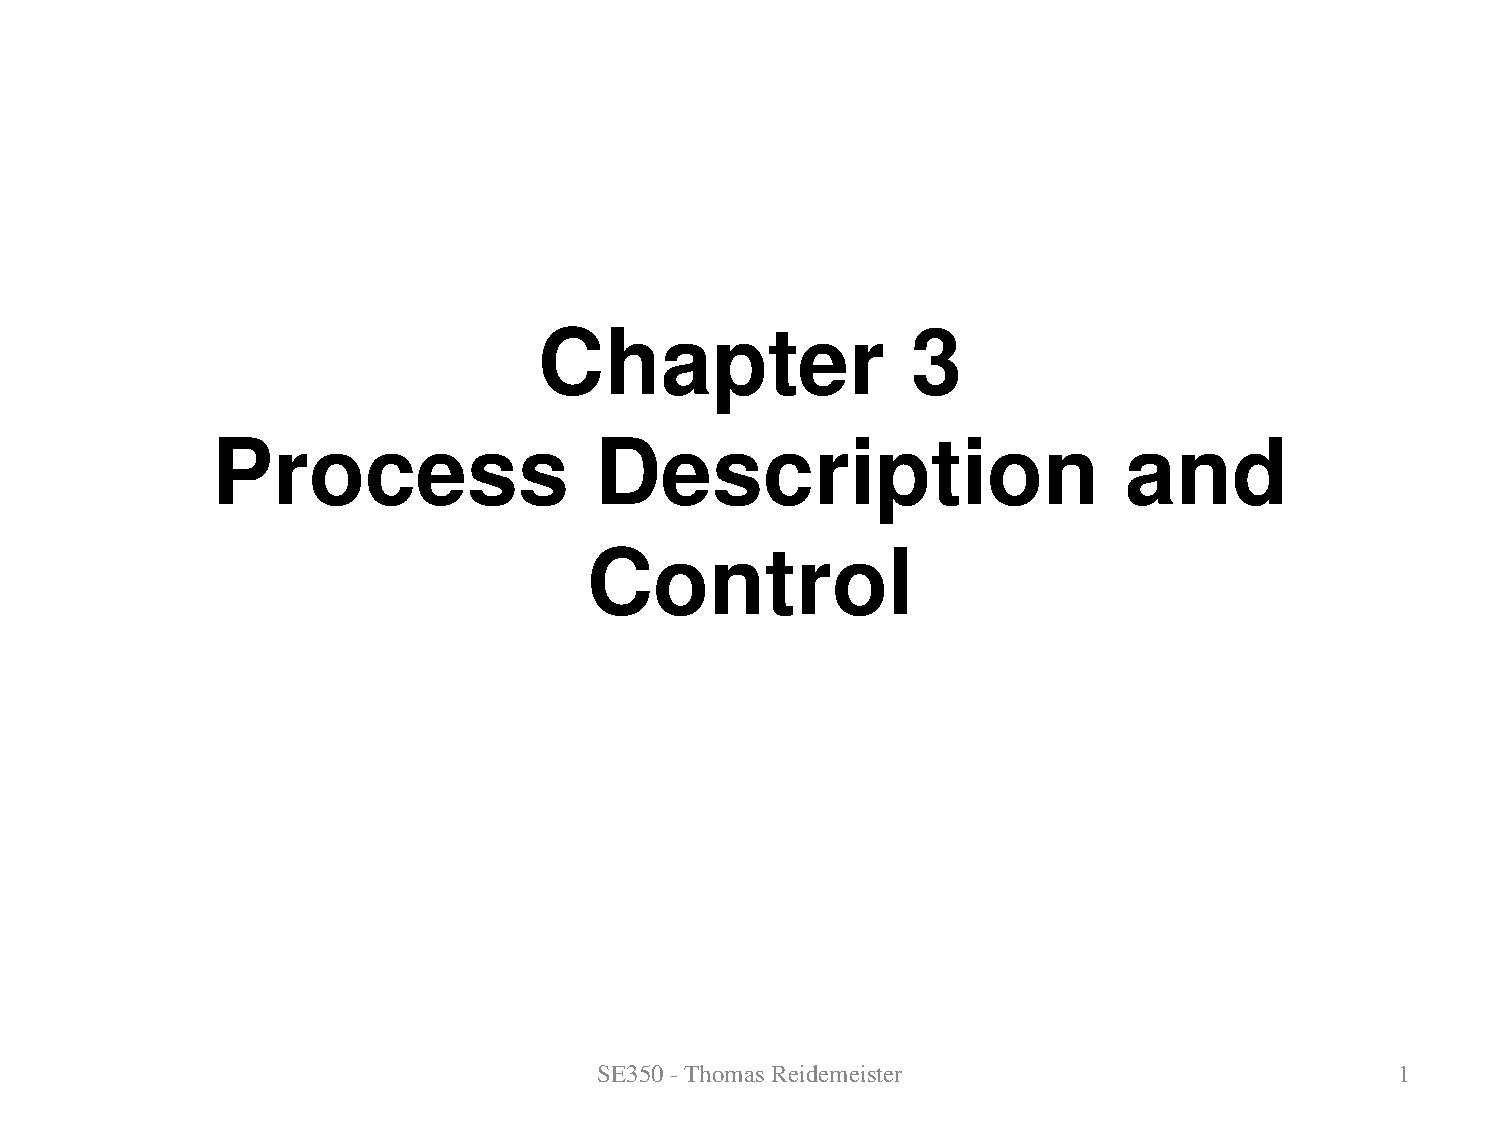
\includepdf[page=25]{03.pdf}
\begin{itemize}
    \item Ready = the process has been set up
    \item Running = the process is currently running
    \item Blocked = the process is waiting for something (like an io read)
    \item New = The memory is not yet fully in memory
    \item Exit = The clean up after process has terminated
\end{itemize}
This state manchine is managed by the dispatcher. We will need a more complicated queue system to manage all of this.

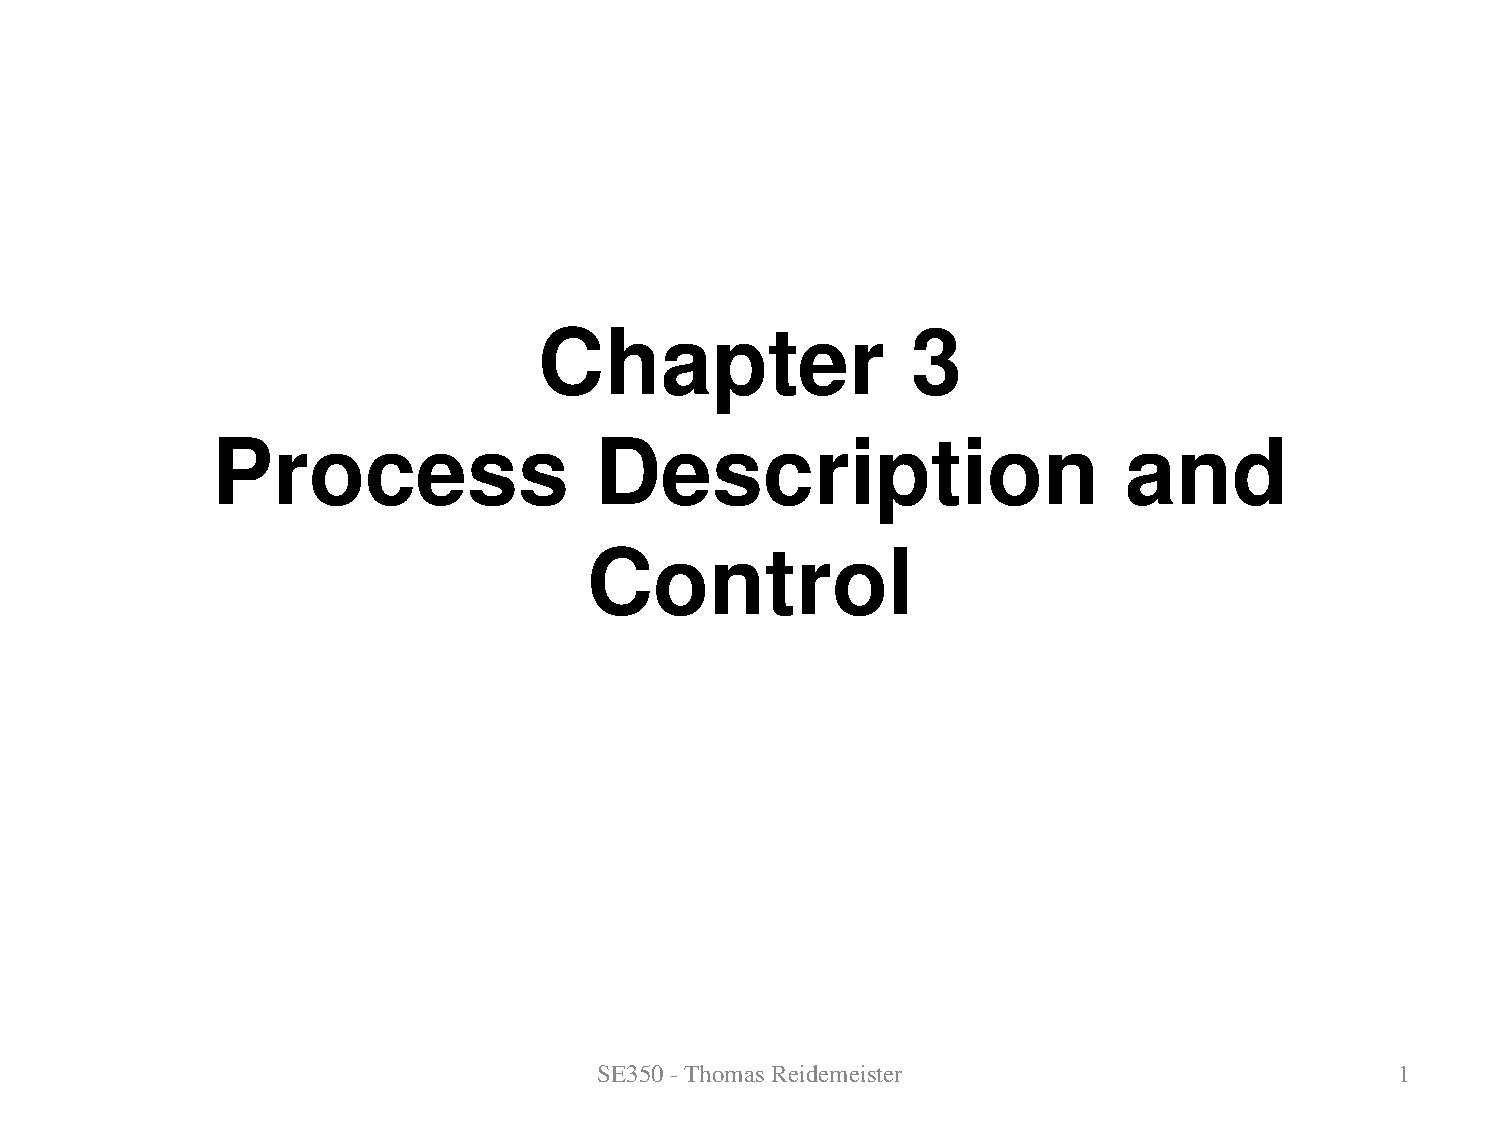
\includepdf[page=26]{03.pdf}
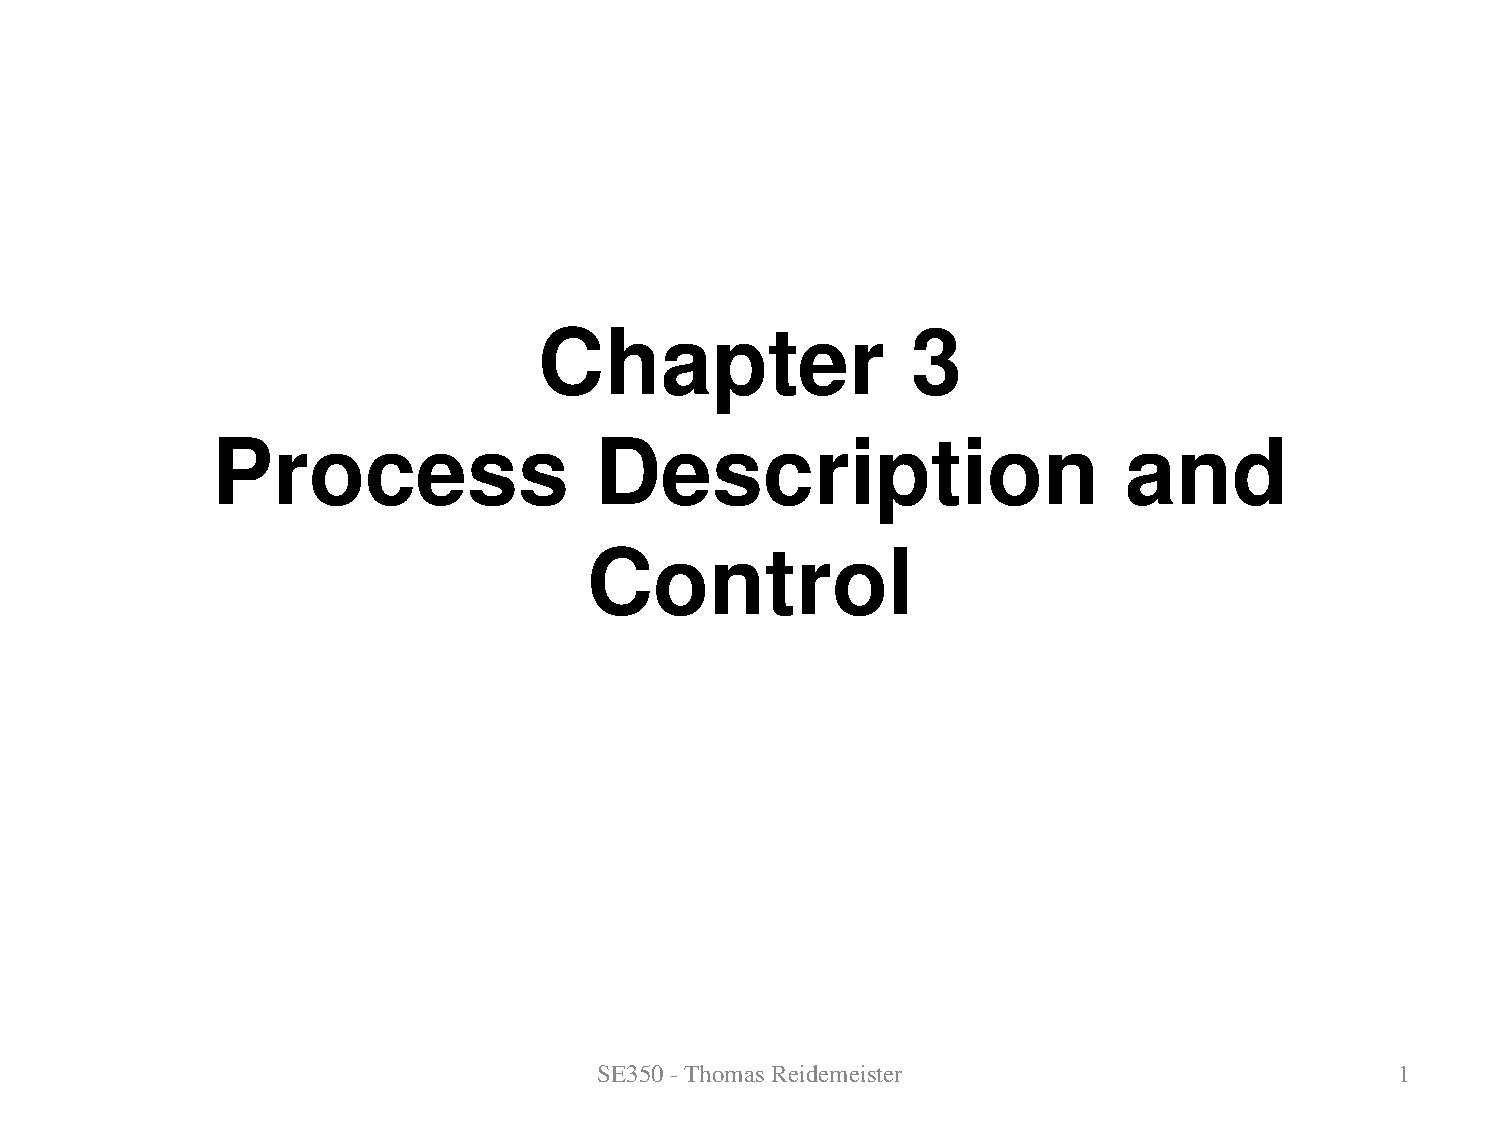
\includepdf[page=27]{03.pdf}
The ready queue has all of the processes ready to run (ie. of that state). Then the dispatcher executes for reasons stated above, it grabs the next ready process. When that process leaves the running state the processor is released and starts again. If the process is blocked it goes onto a blocked queue which then goes back to be admited and pushed onto the bottom of the ready queue. This also allows for timeouts to kick a stalled process back onto the wait queue to free the processor. The problem with this design is that there will be many IO's.

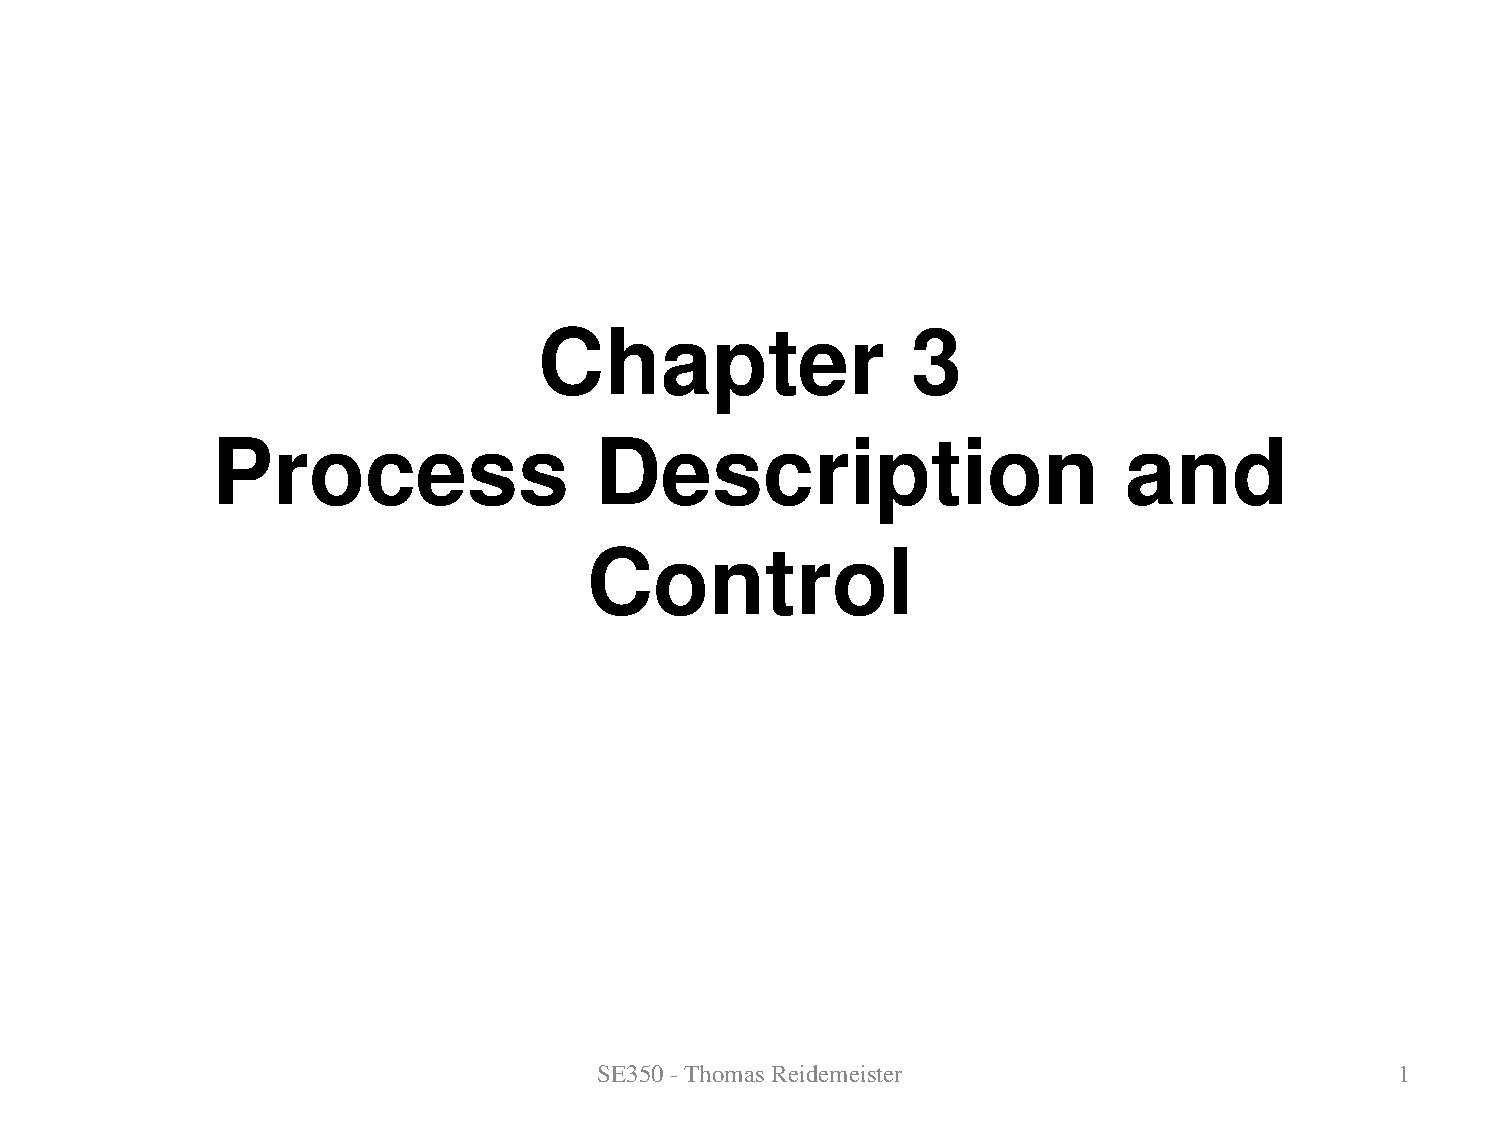
\includepdf[page=28]{03.pdf}
To deal with inefficiencies of multiple of IO's we make a queue for each IO. Every time a specific event occurs it the processor puts it onto that specific queues to wait there and just pop off the top one when its done. Now we dont have to look for a specific process when it's specific ready call is done. So if two different blocks happen they go onto two different queues that each wait for their own unblock signal when previously we would have to search through the block queue for the correct process.

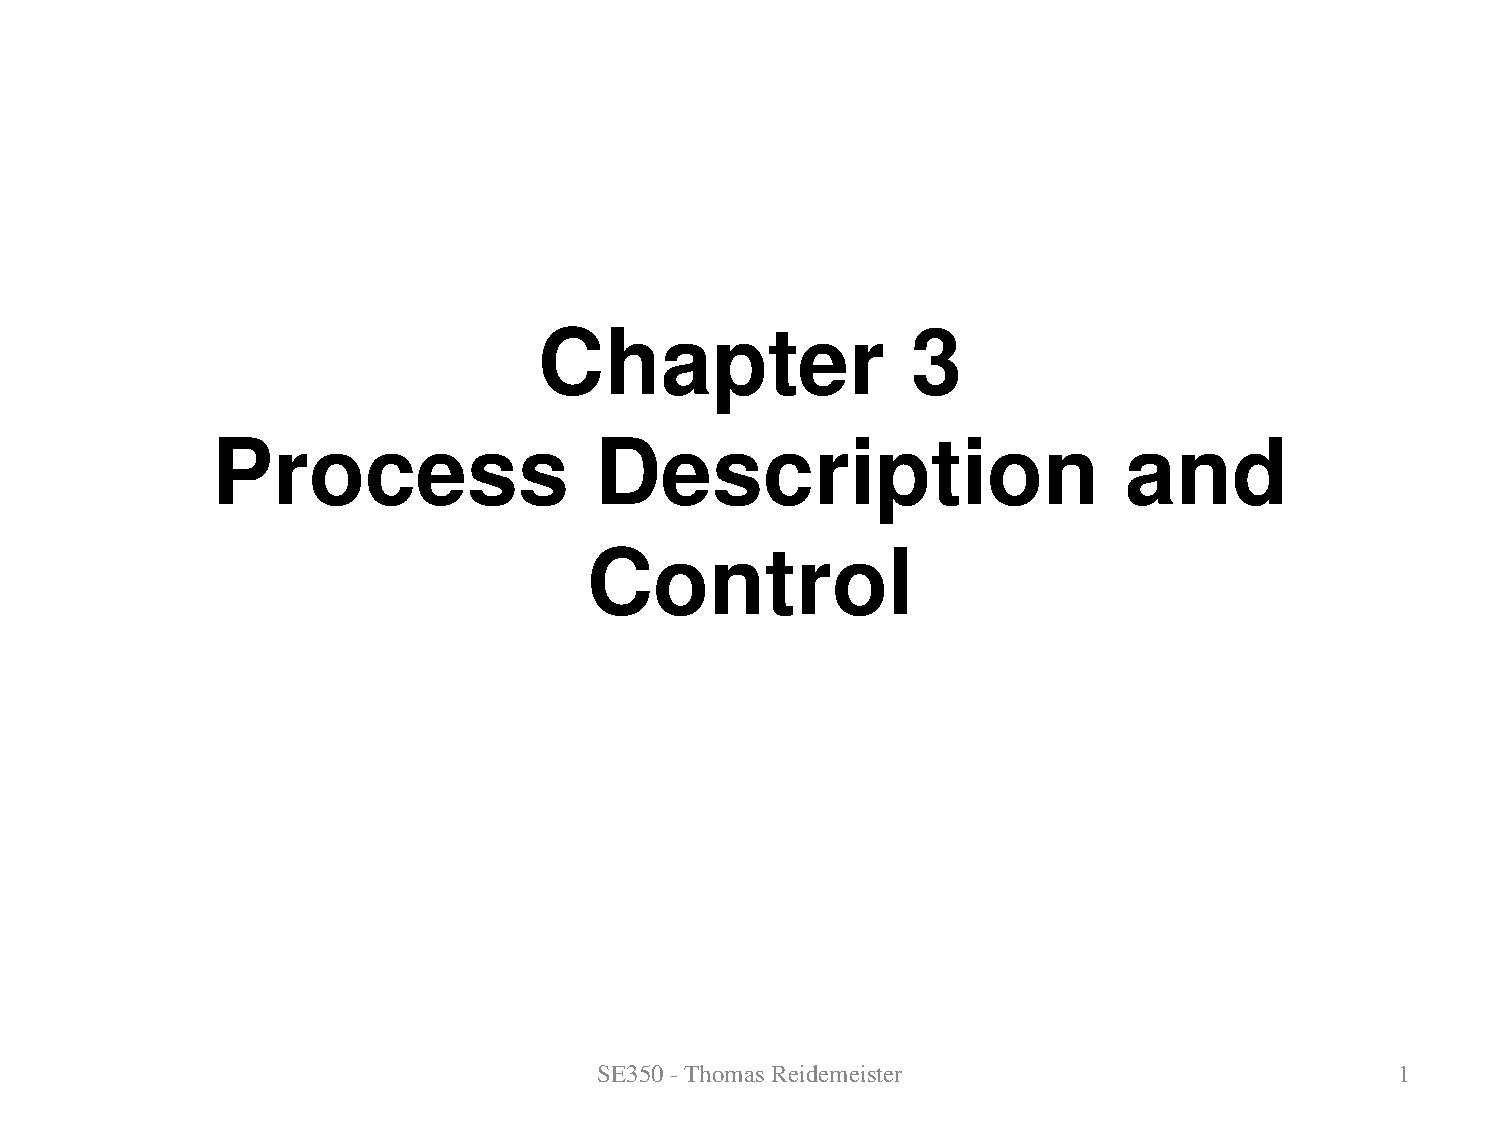
\includepdf[page=29]{03.pdf}
We added a suspended state to allow us to admit more processes. This is when the program is paused to free up more memory on the stack. For a program to be running it needs to be loaded into main memory.
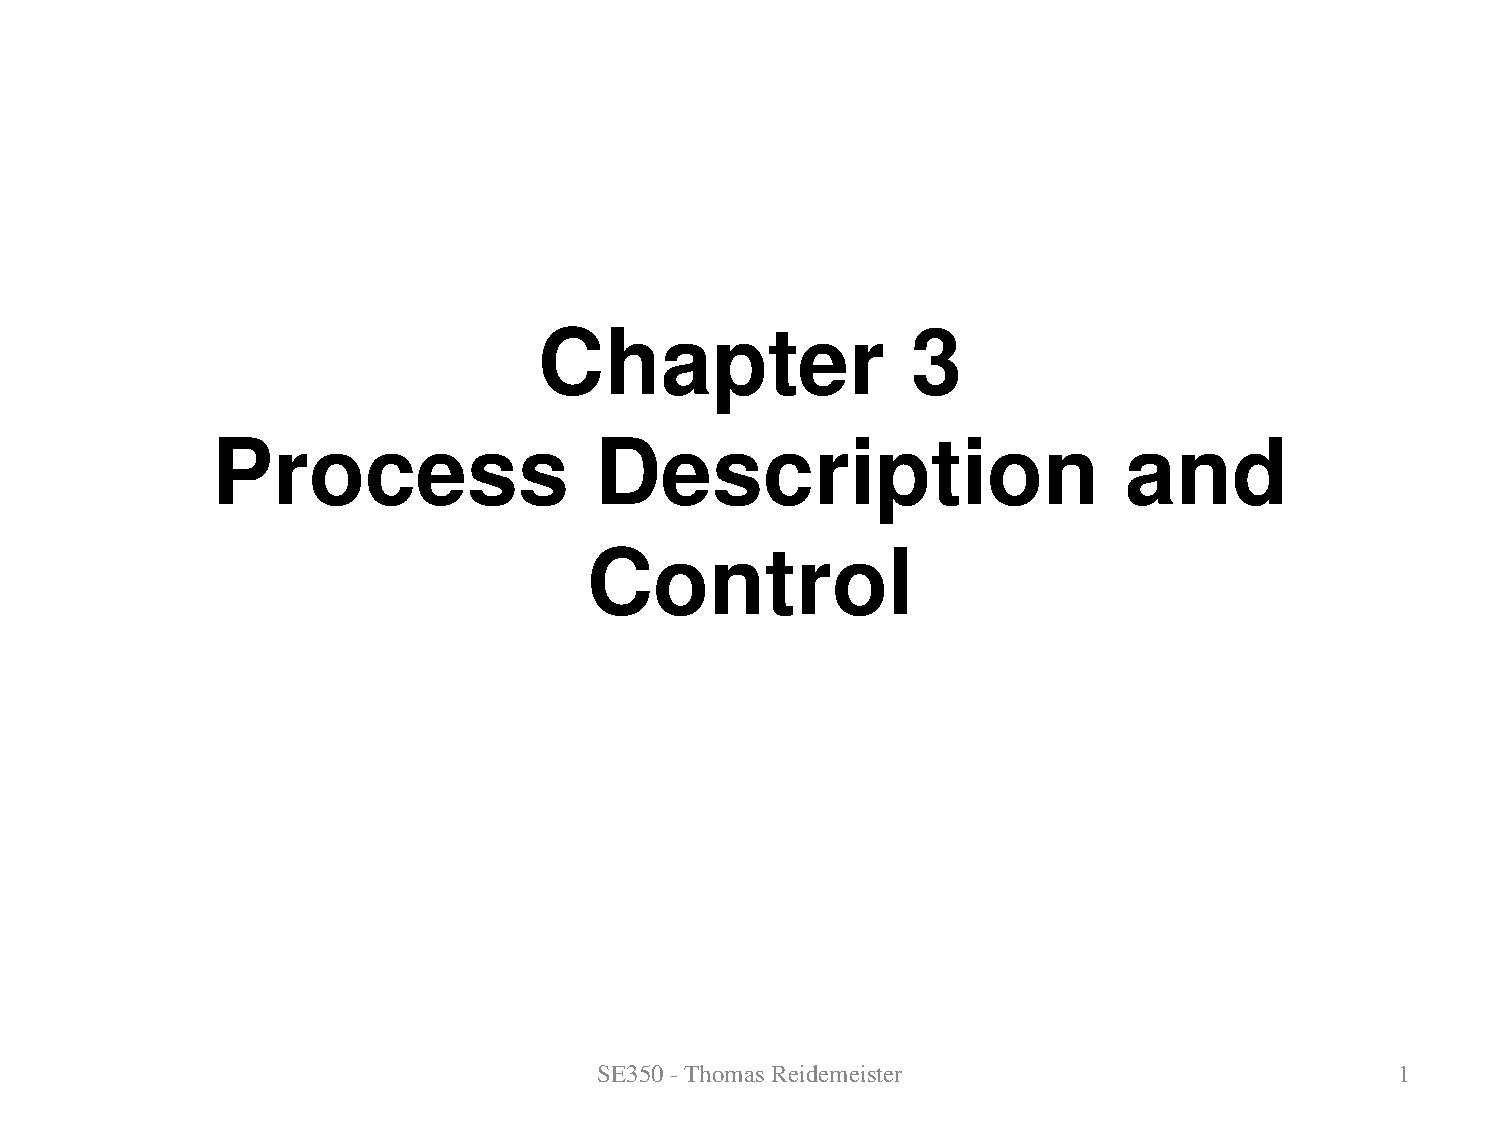
\includepdf[page=30]{03.pdf}
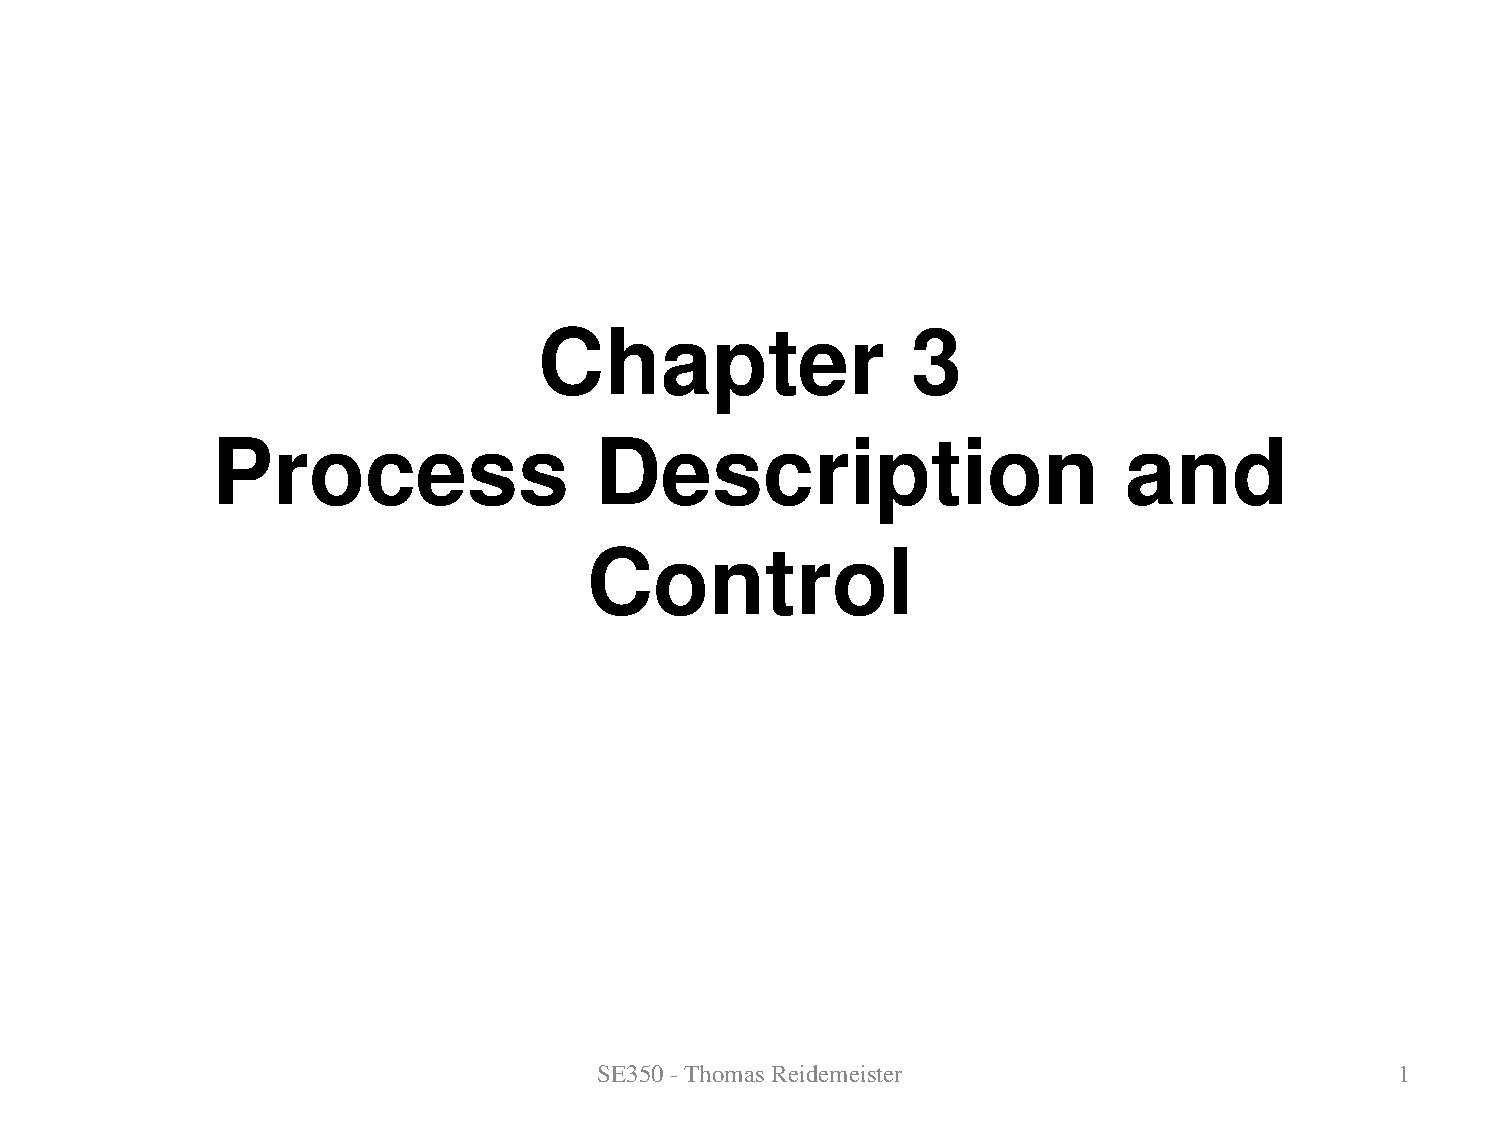
\includepdf[page=31]{03.pdf}
If we have memory available it goes to the ready state, else it goes to the suspend state and none of the necissary stuff is loaded into memory. When there is enough space we put it into the ready queue to be executed like normal. We have a similar queue when a blocked process tries to enter the ready queue and cannot. This lets us admit as many processors as possible into our system without memory being a constraint.
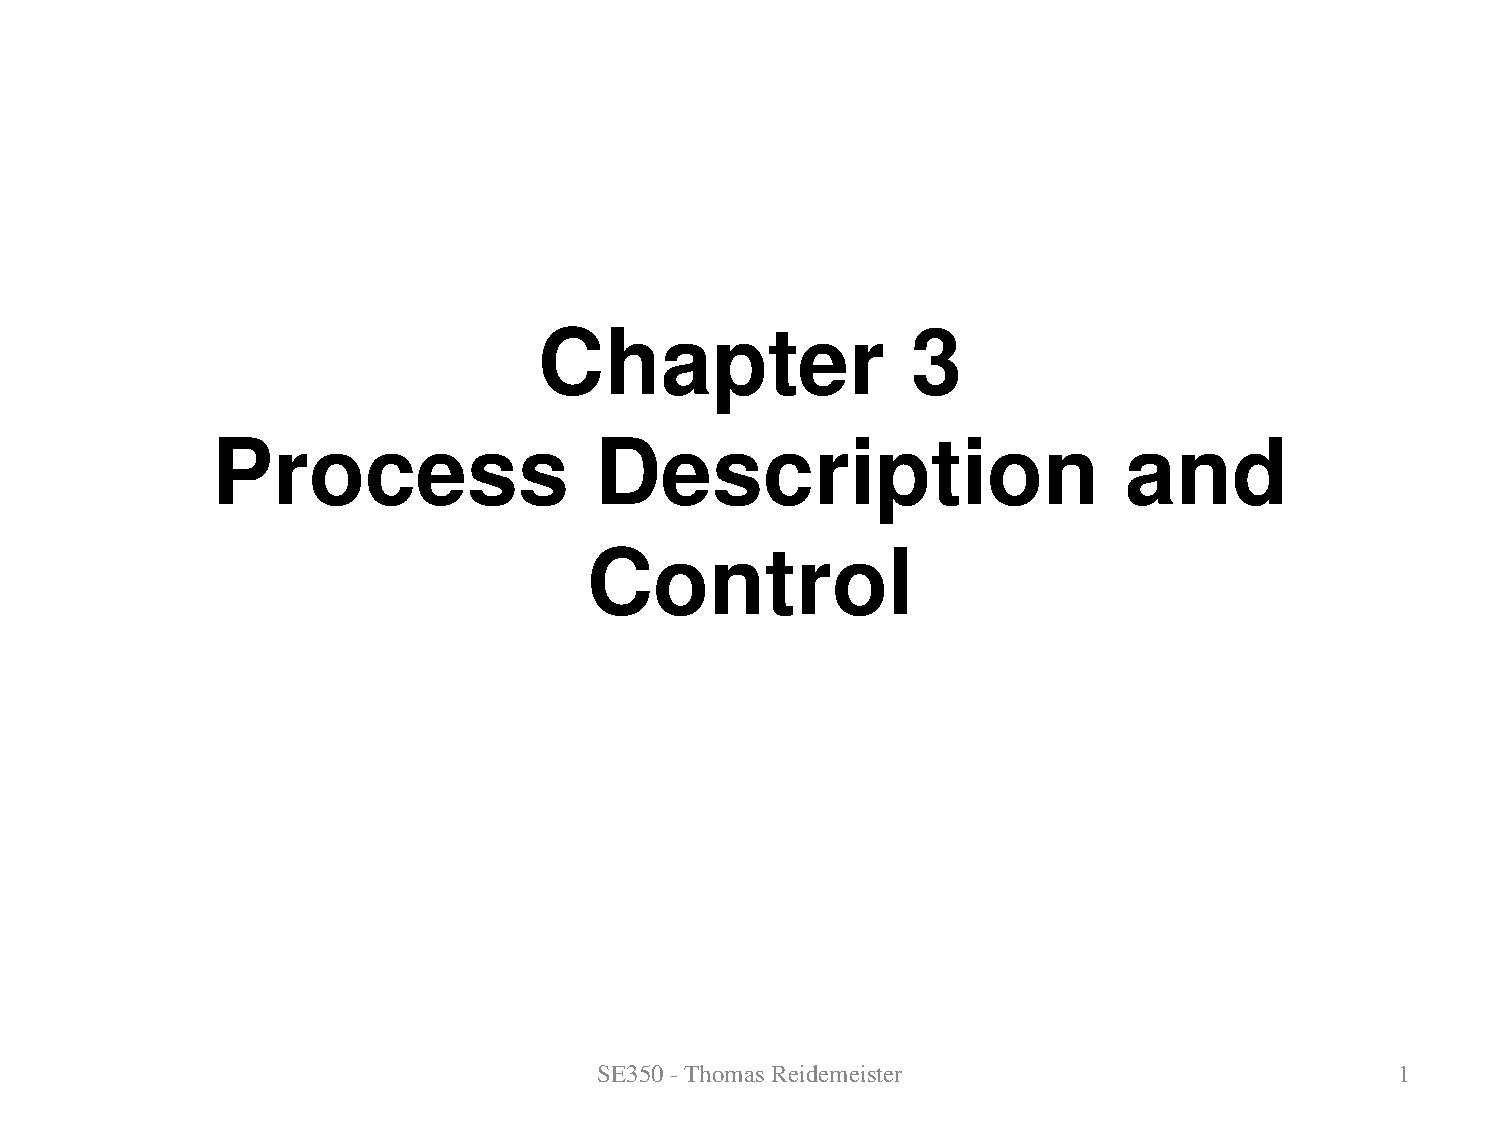
\includepdf[page=32]{03.pdf}
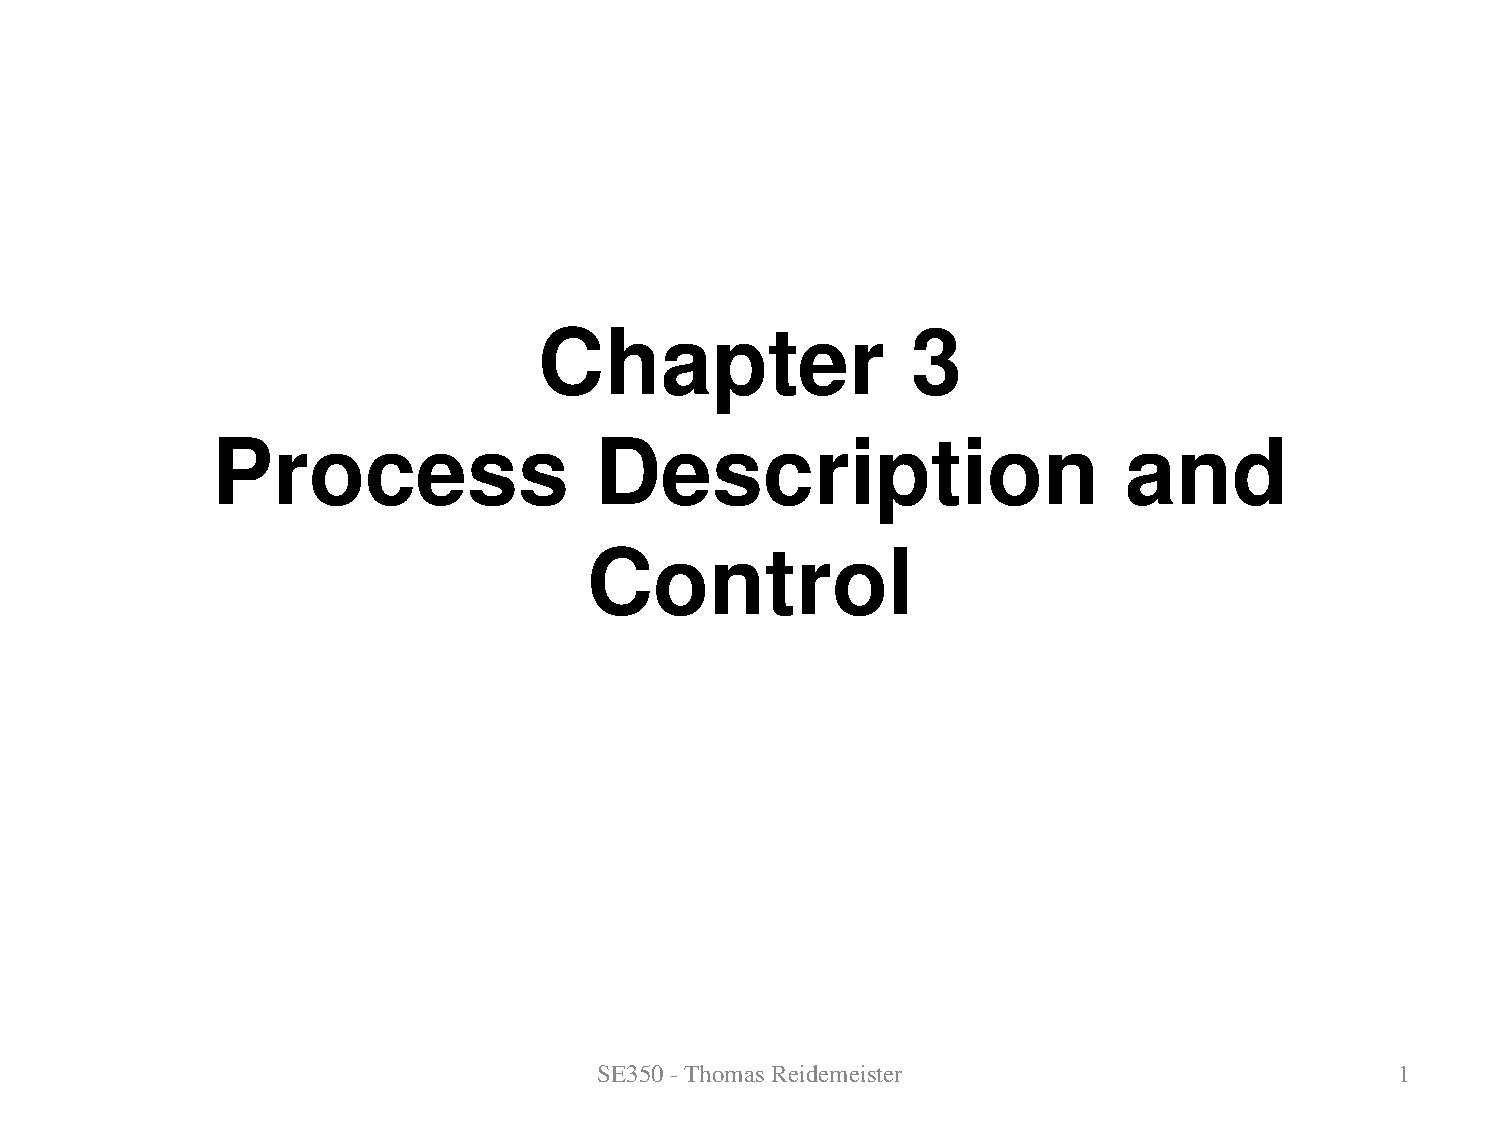
\includepdf[page=33]{03.pdf}
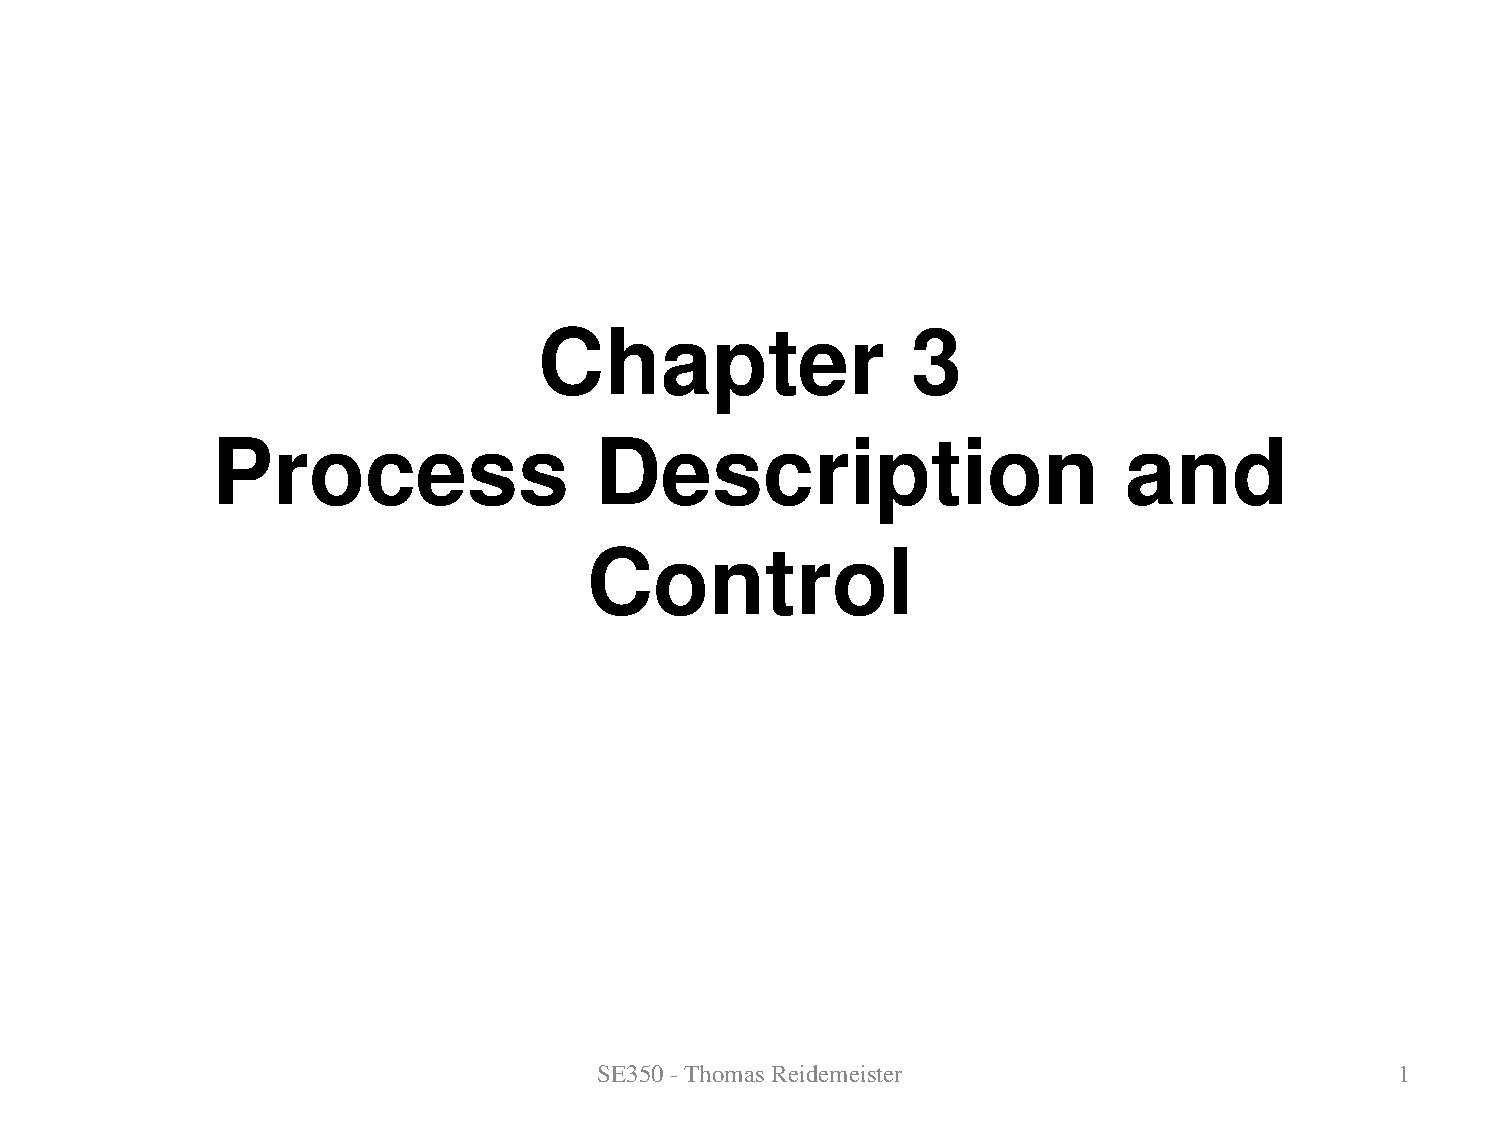
\includepdf[page=34]{03.pdf}
A process is assigned to one or more processors and might use peripherals during its execution. These all need to be managed by the OS.
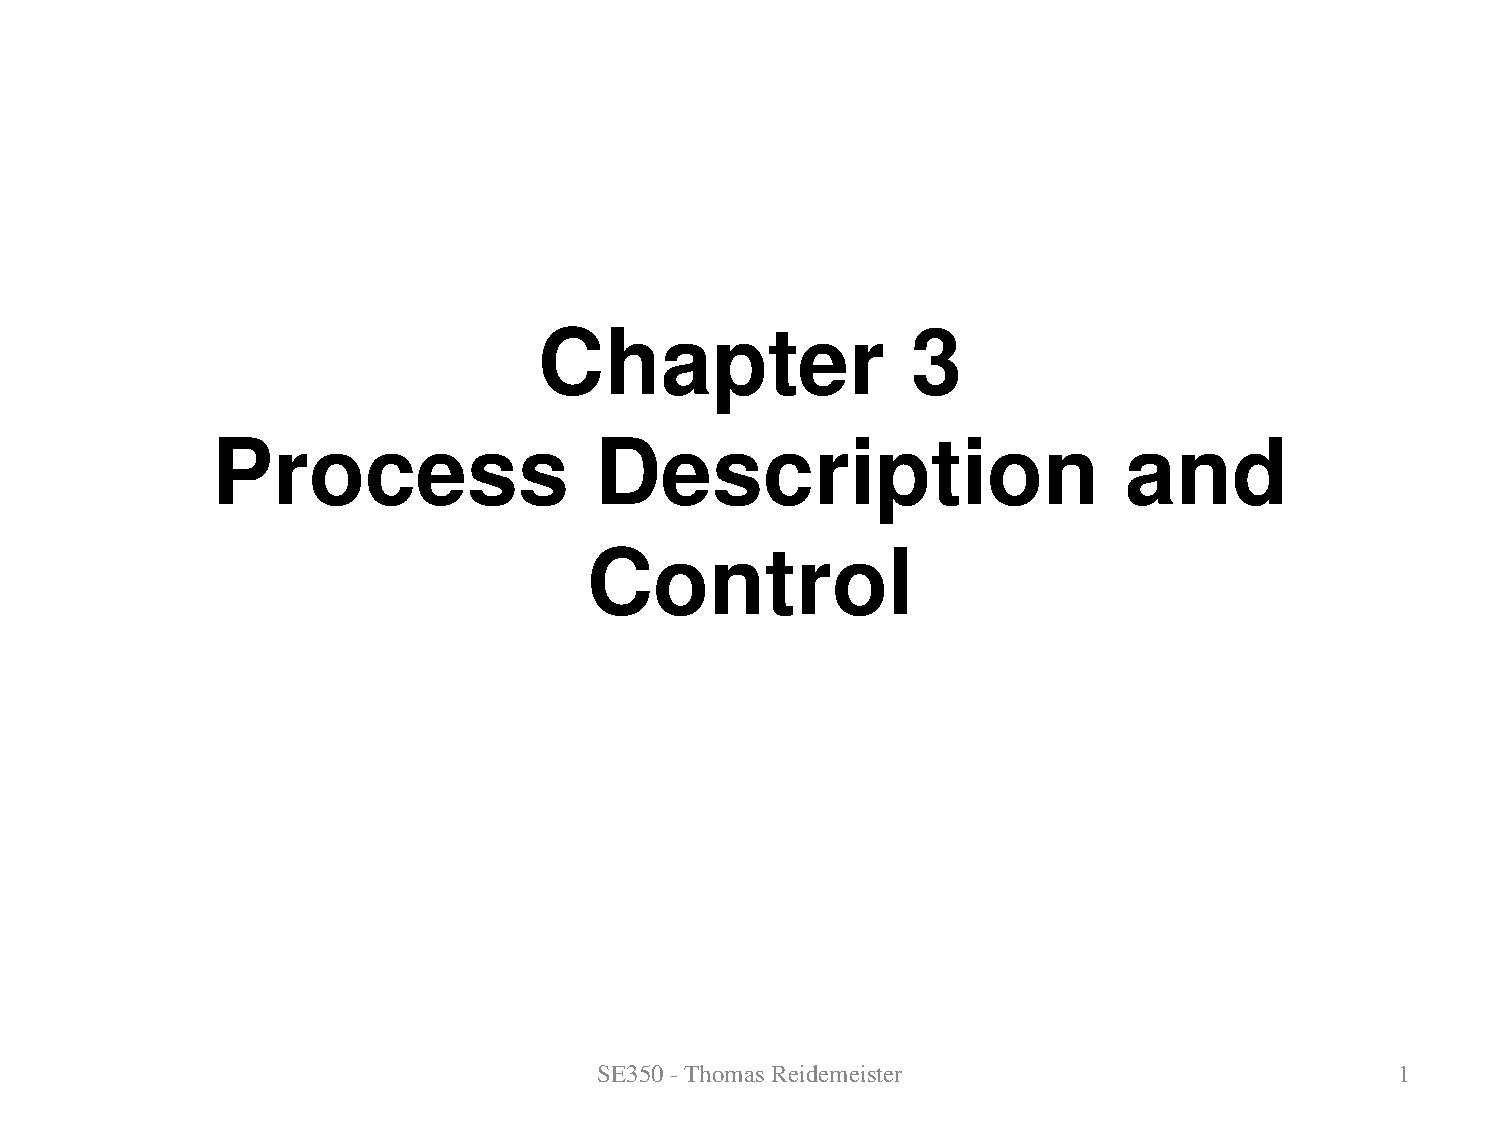
\includepdf[page=35]{03.pdf}
We manage things by storing them in tables with maps.
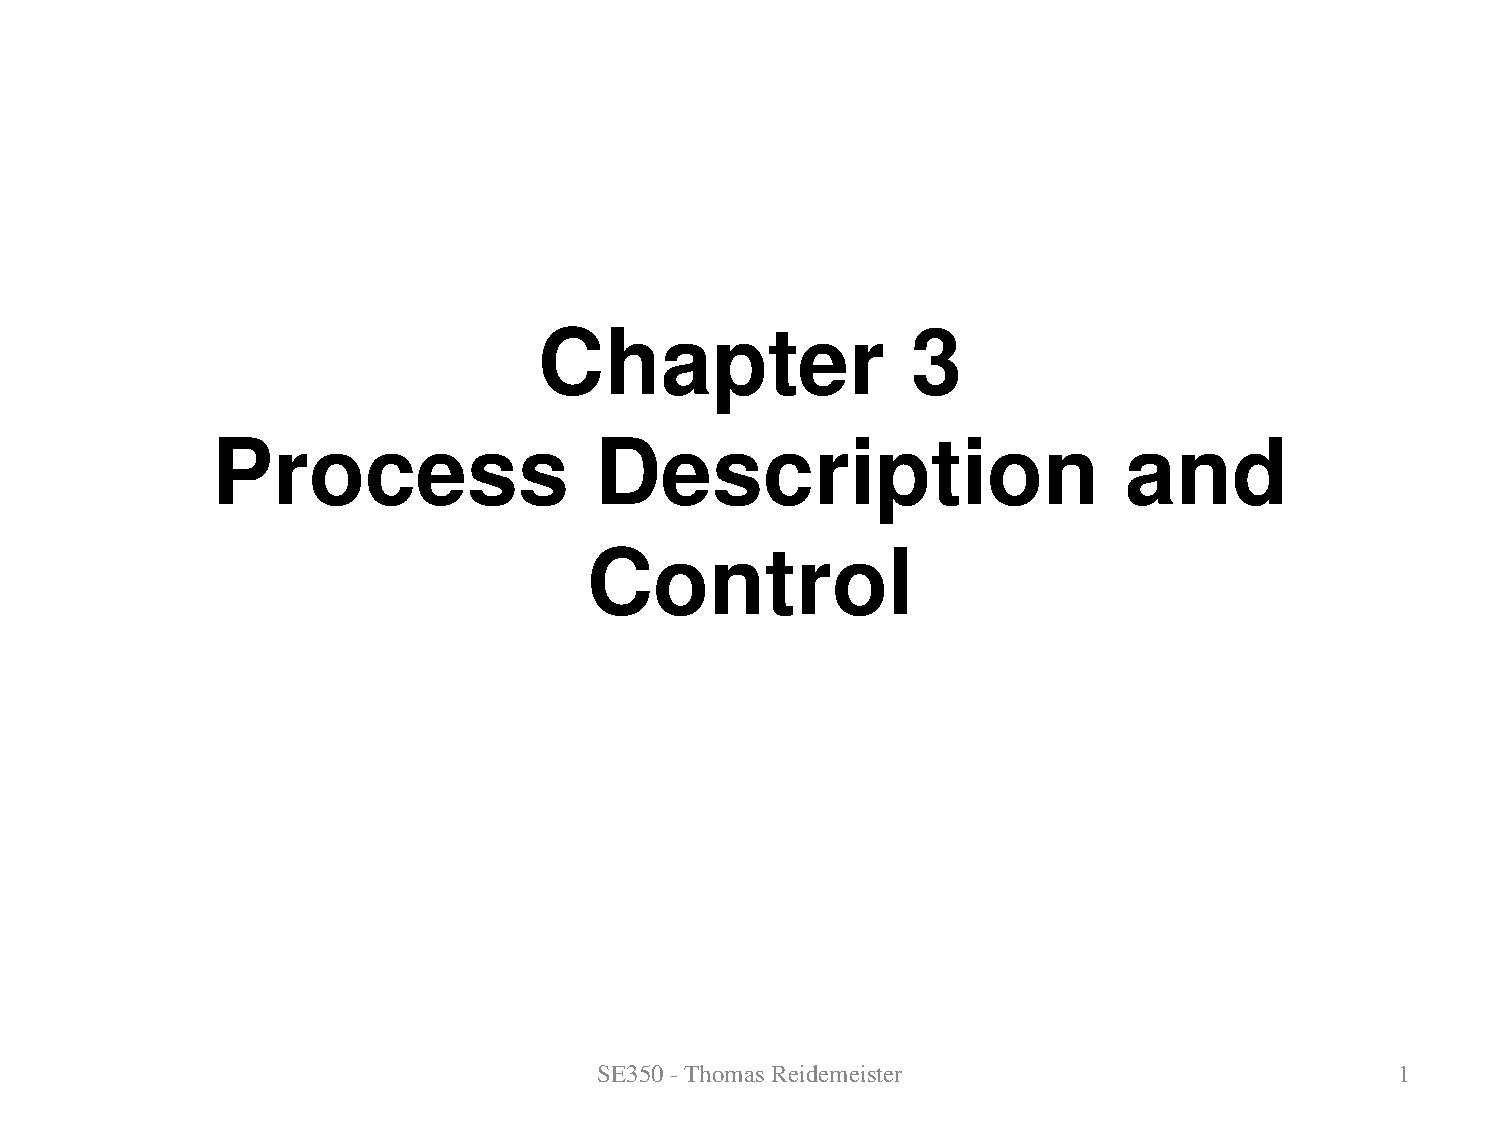
\includepdf[page=36]{03.pdf}
Overtime main memory becomes fragmented which we need to keep track of and what secondary storage is allocated to processes. Ditto for virtual memory.
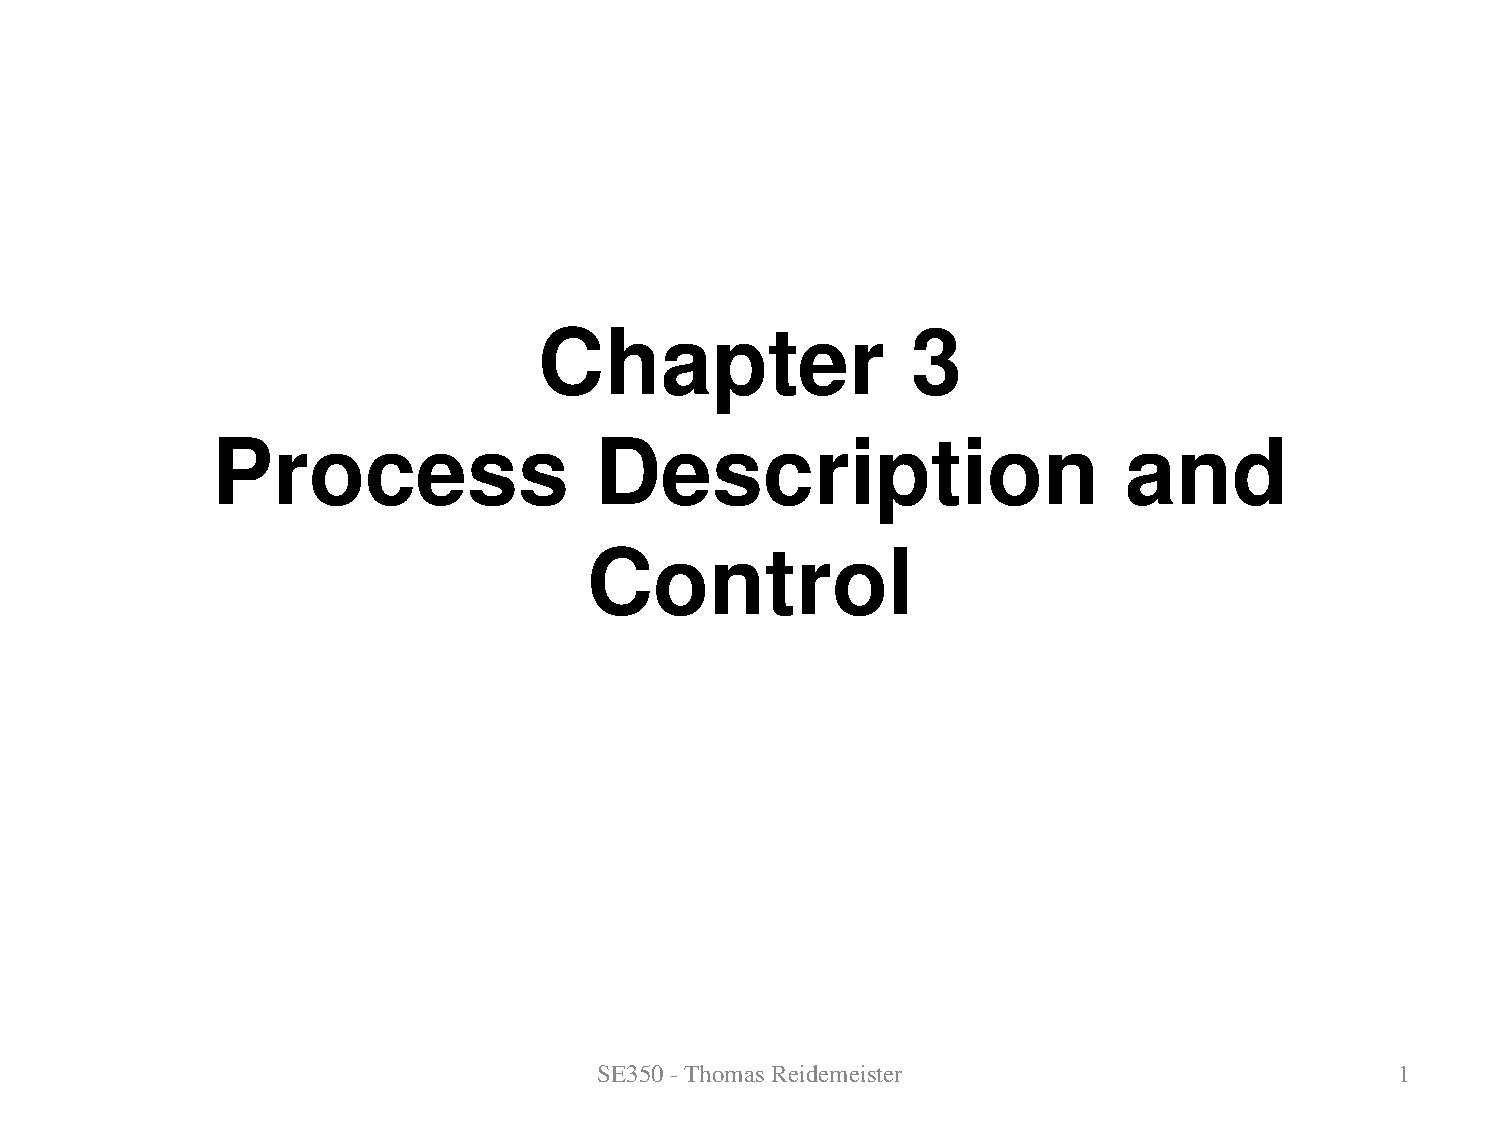
\includepdf[page=37]{03.pdf}
We use IO tables to track which IOs are in use and what memory they are using.
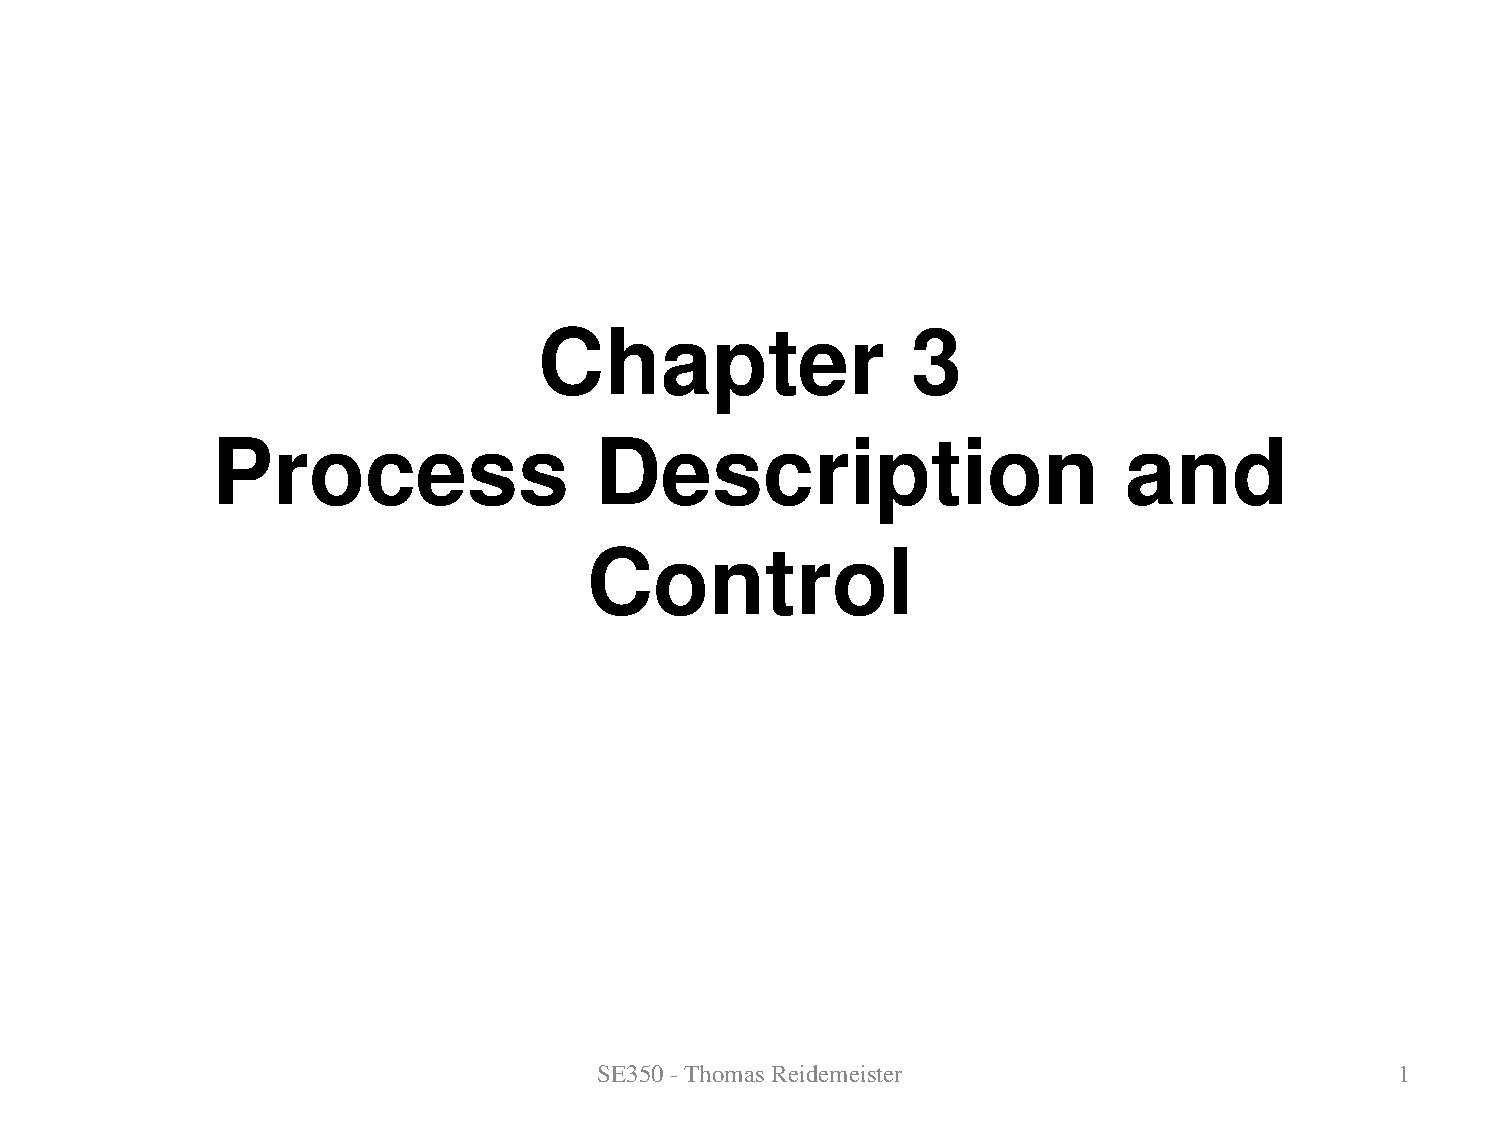
\includepdf[page=38]{03.pdf}
What files are allocated, their location, protection attributes, and what process they are locked to.
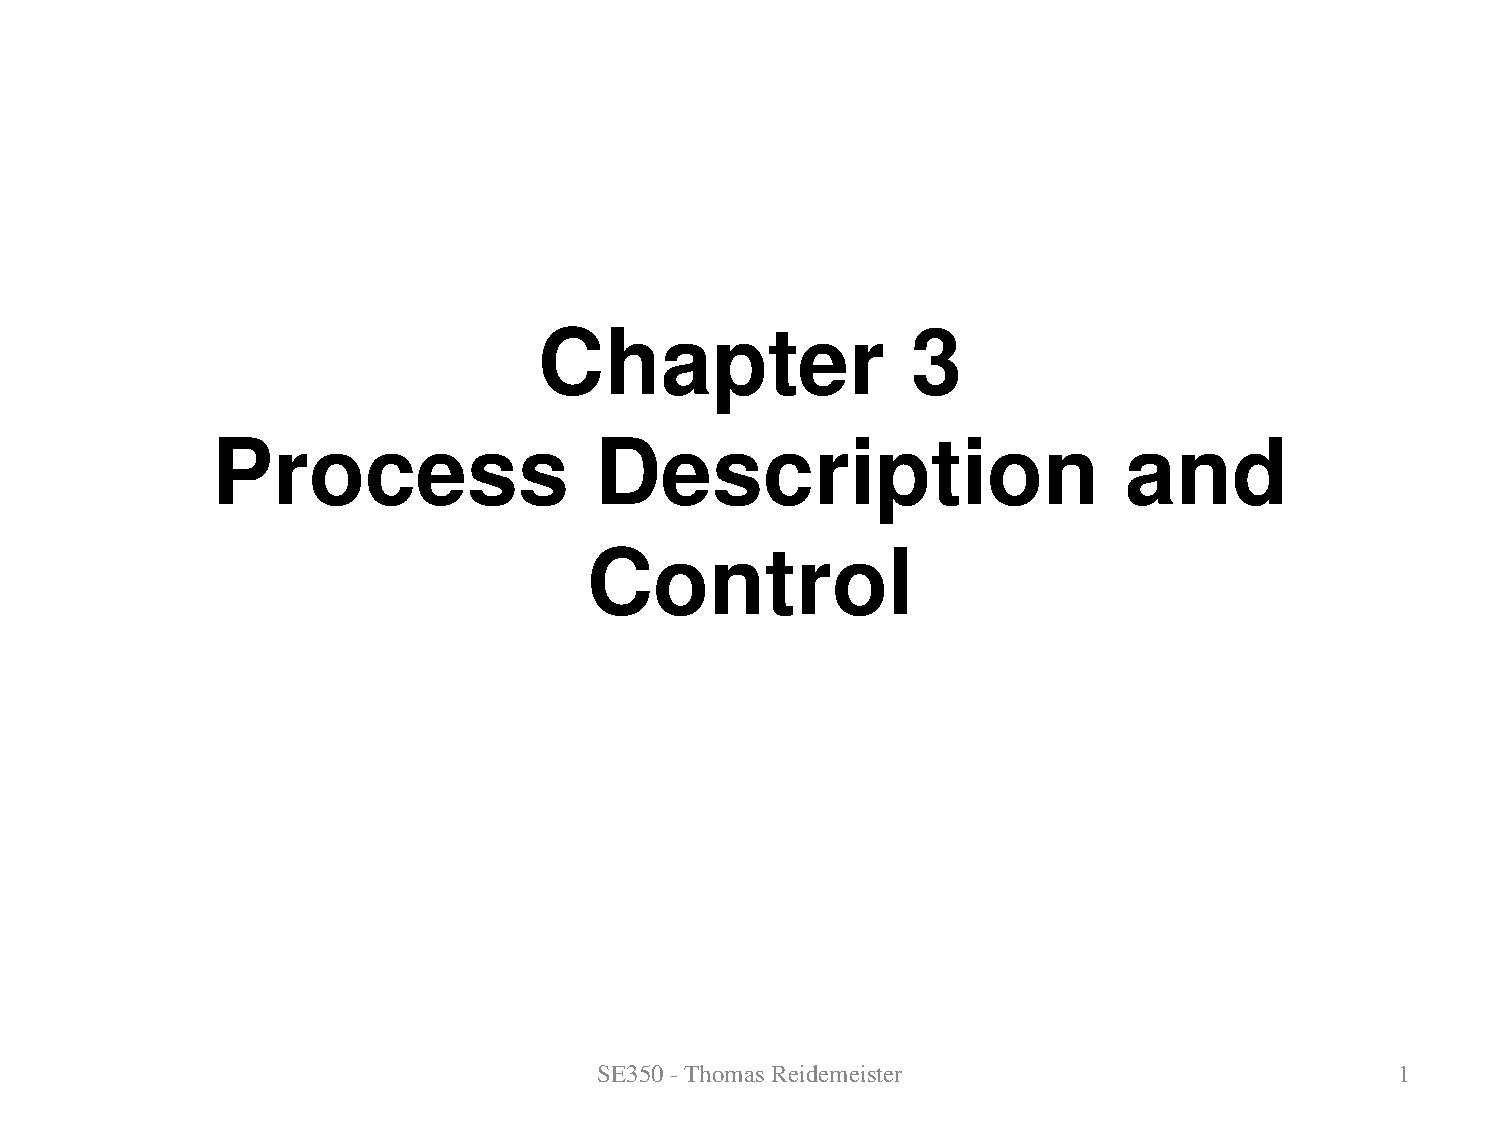
\includepdf[page=39]{03.pdf}
A process table stores the id, where the process is in memory, its attributes, what data it uses, its stack start, and the process control block. All of the above listed tables are created during boot time and saved at shut down.
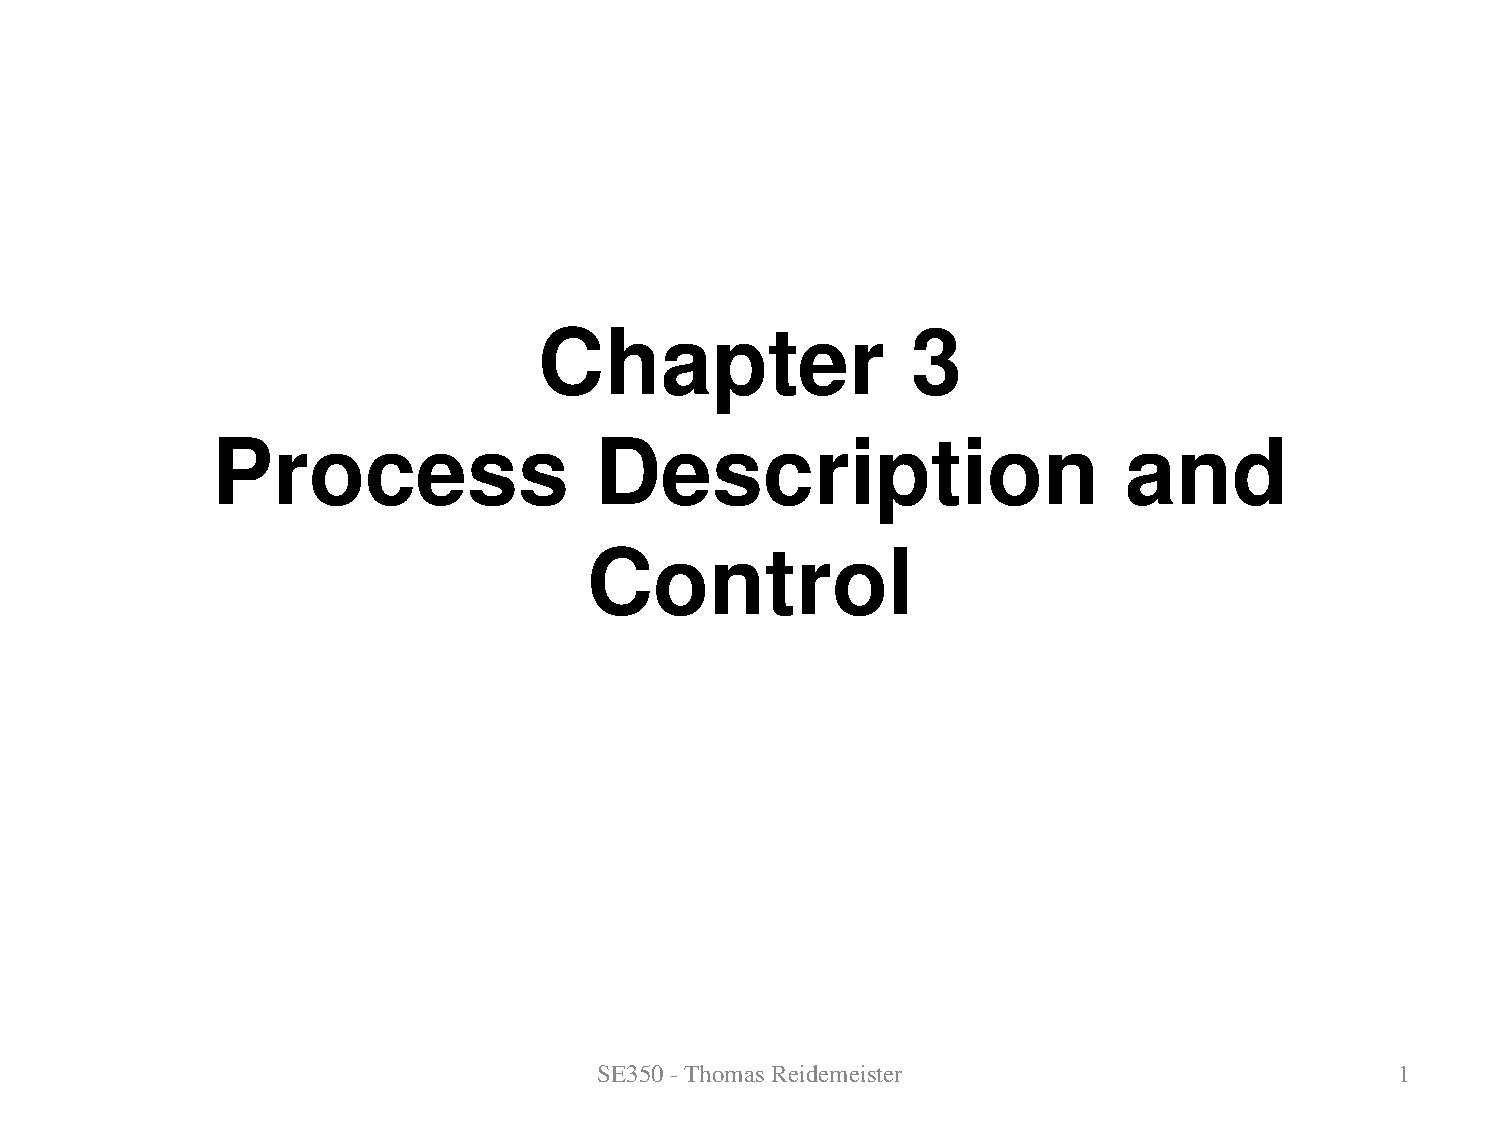
\includepdf[page=40]{03.pdf}
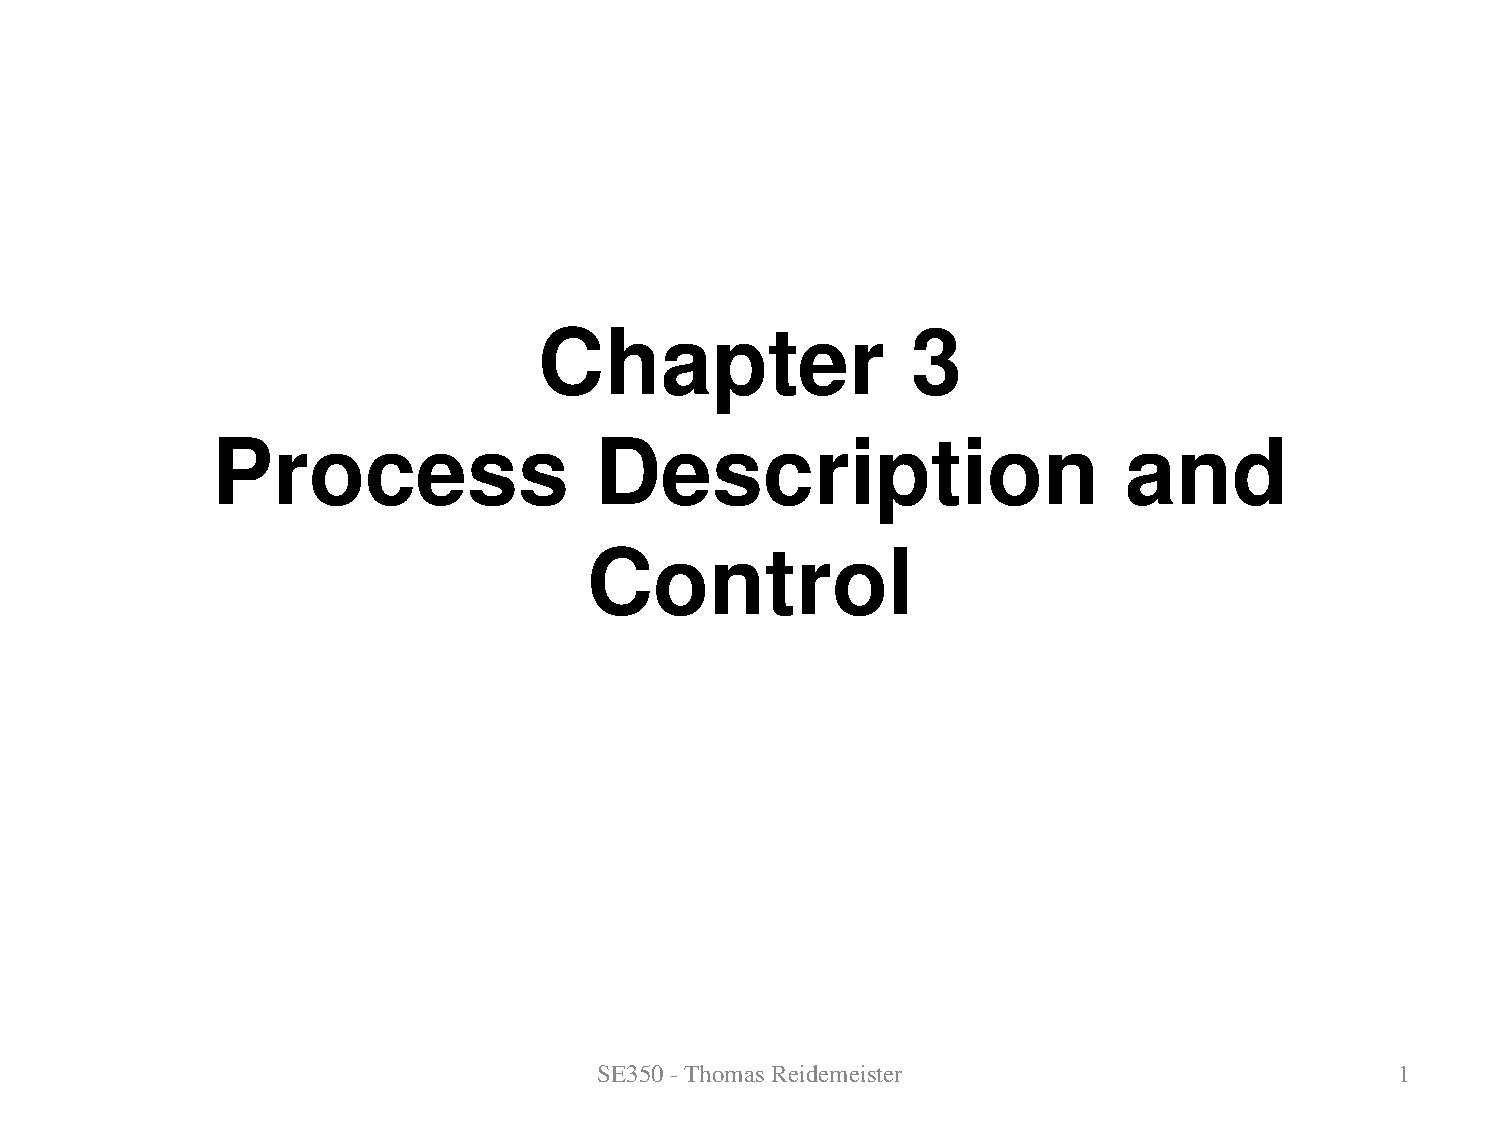
\includepdf[page=41]{03.pdf}
This is a overview of the process table implementation. For each of the resources we have a table which are initialized at boot. For processes the table contains links to the process image.
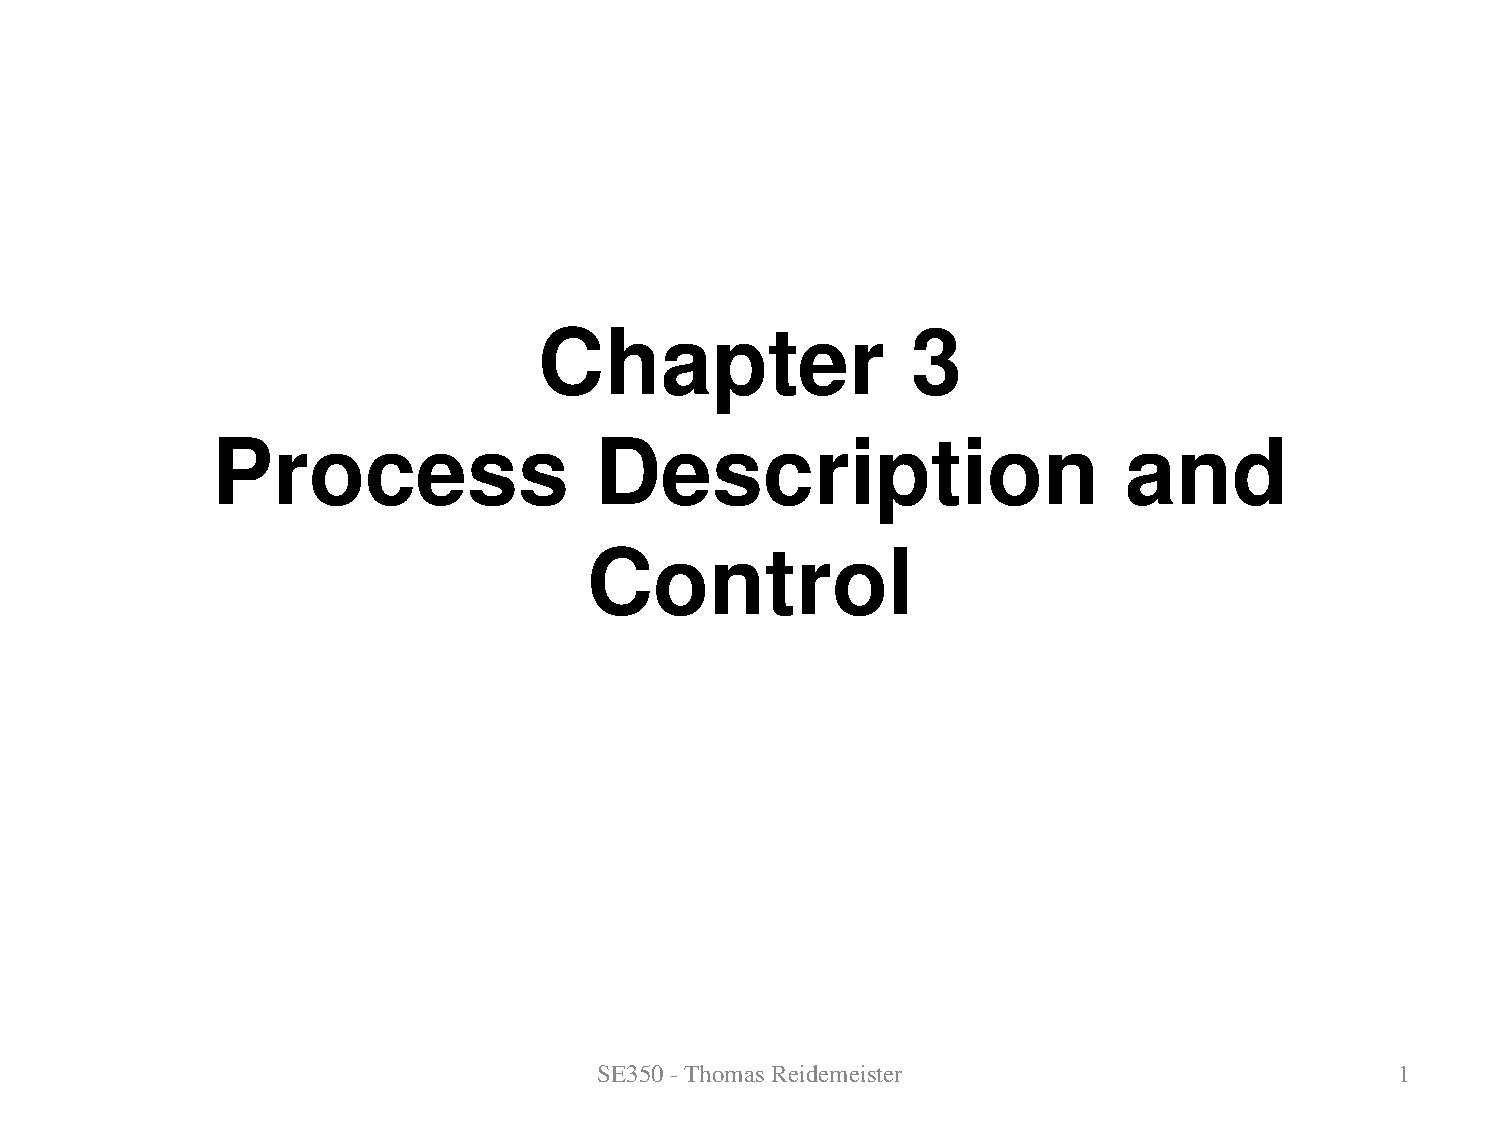
\includepdf[page=42]{03.pdf}
Process Identification(PID): when you have processes that spawn processes you need to keep track of what their parents are. Processes that are started during boot time are mapped to process one. There is a sequence counter that generates the PID.
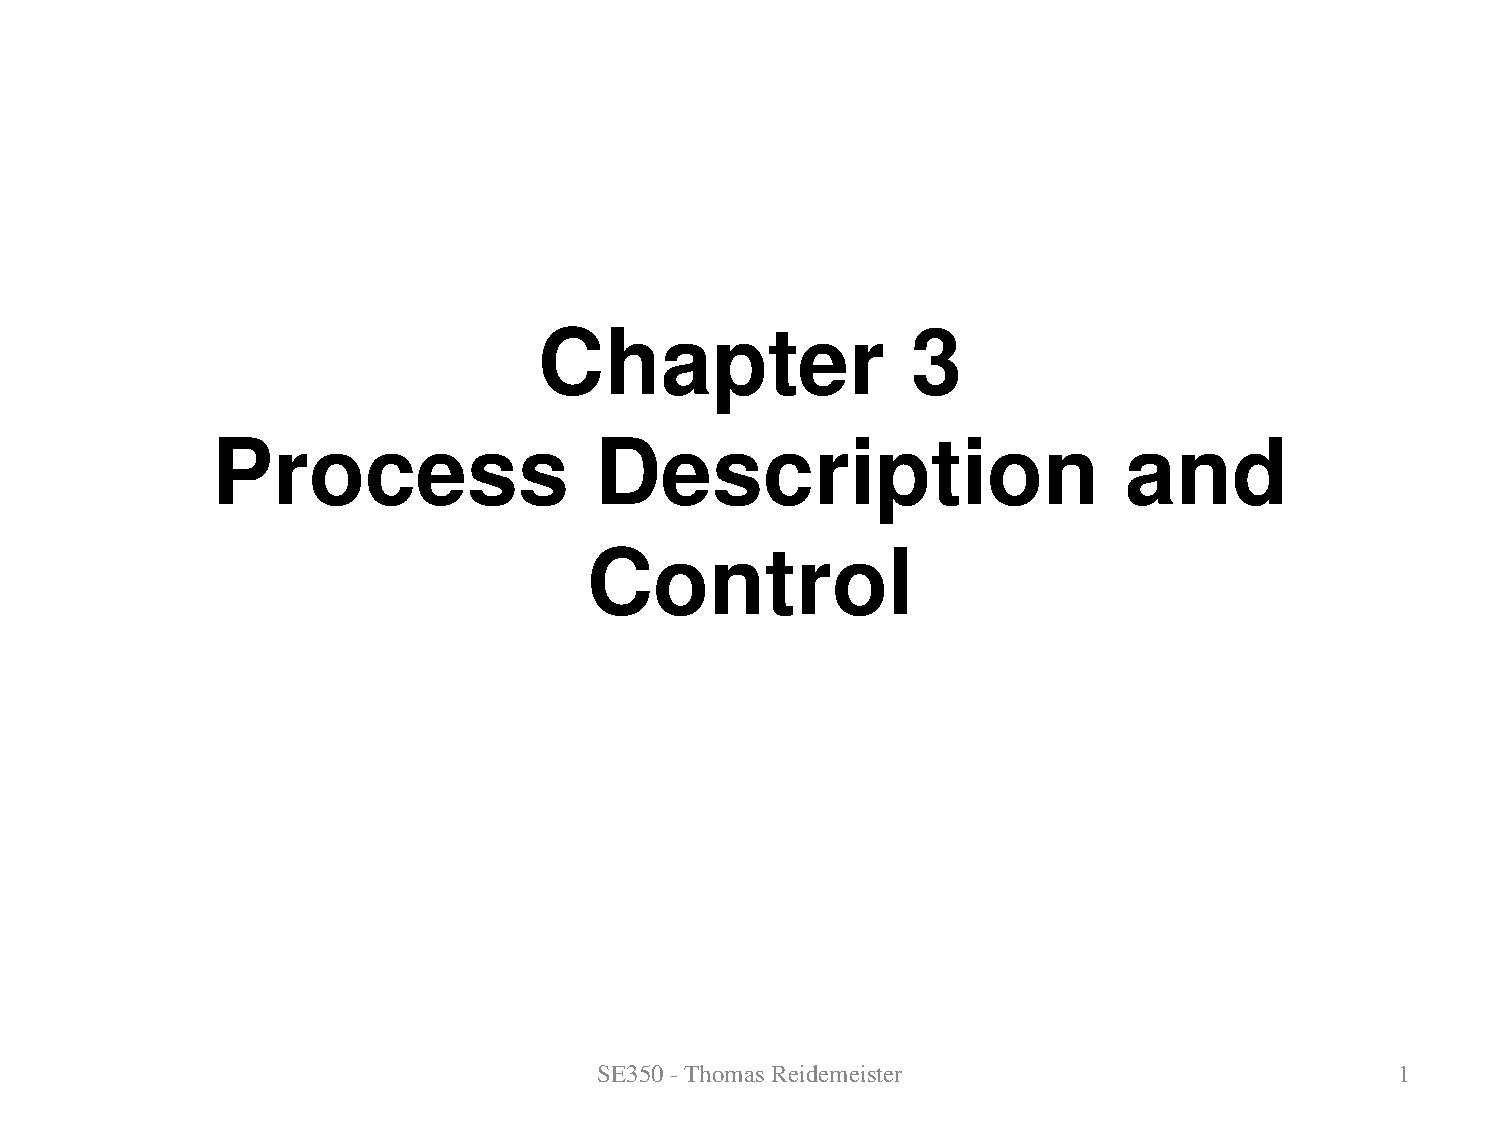
\includepdf[page=43]{03.pdf}
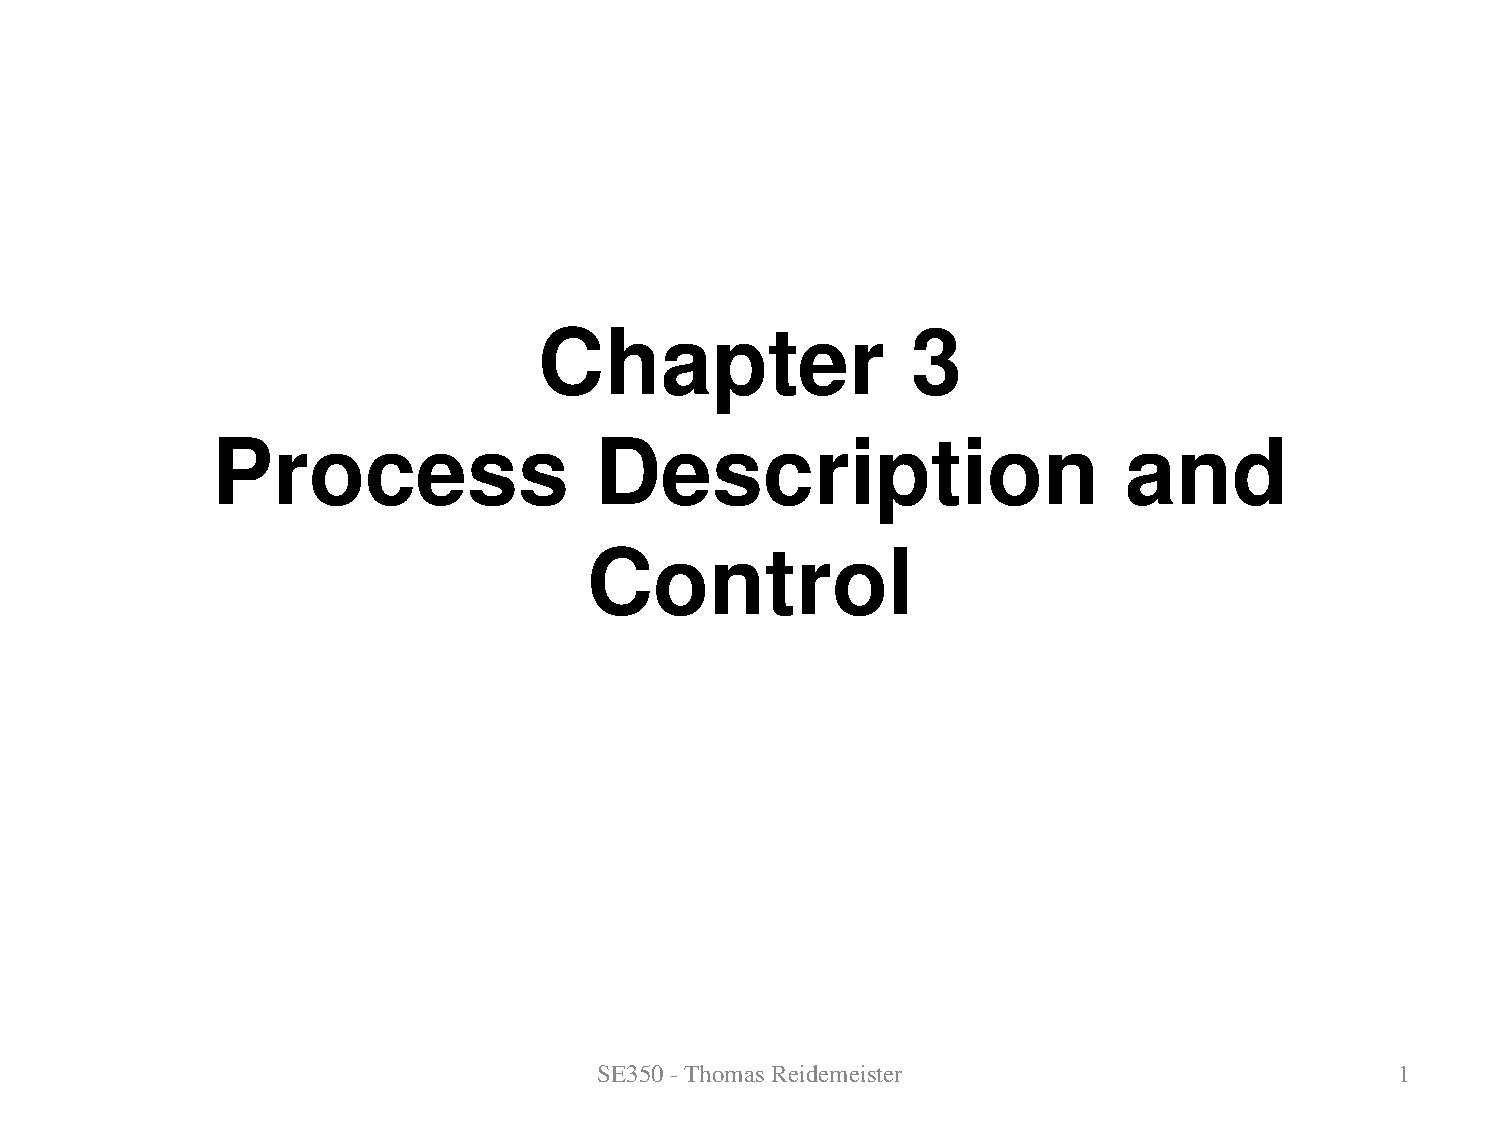
\includepdf[page=44]{03.pdf}
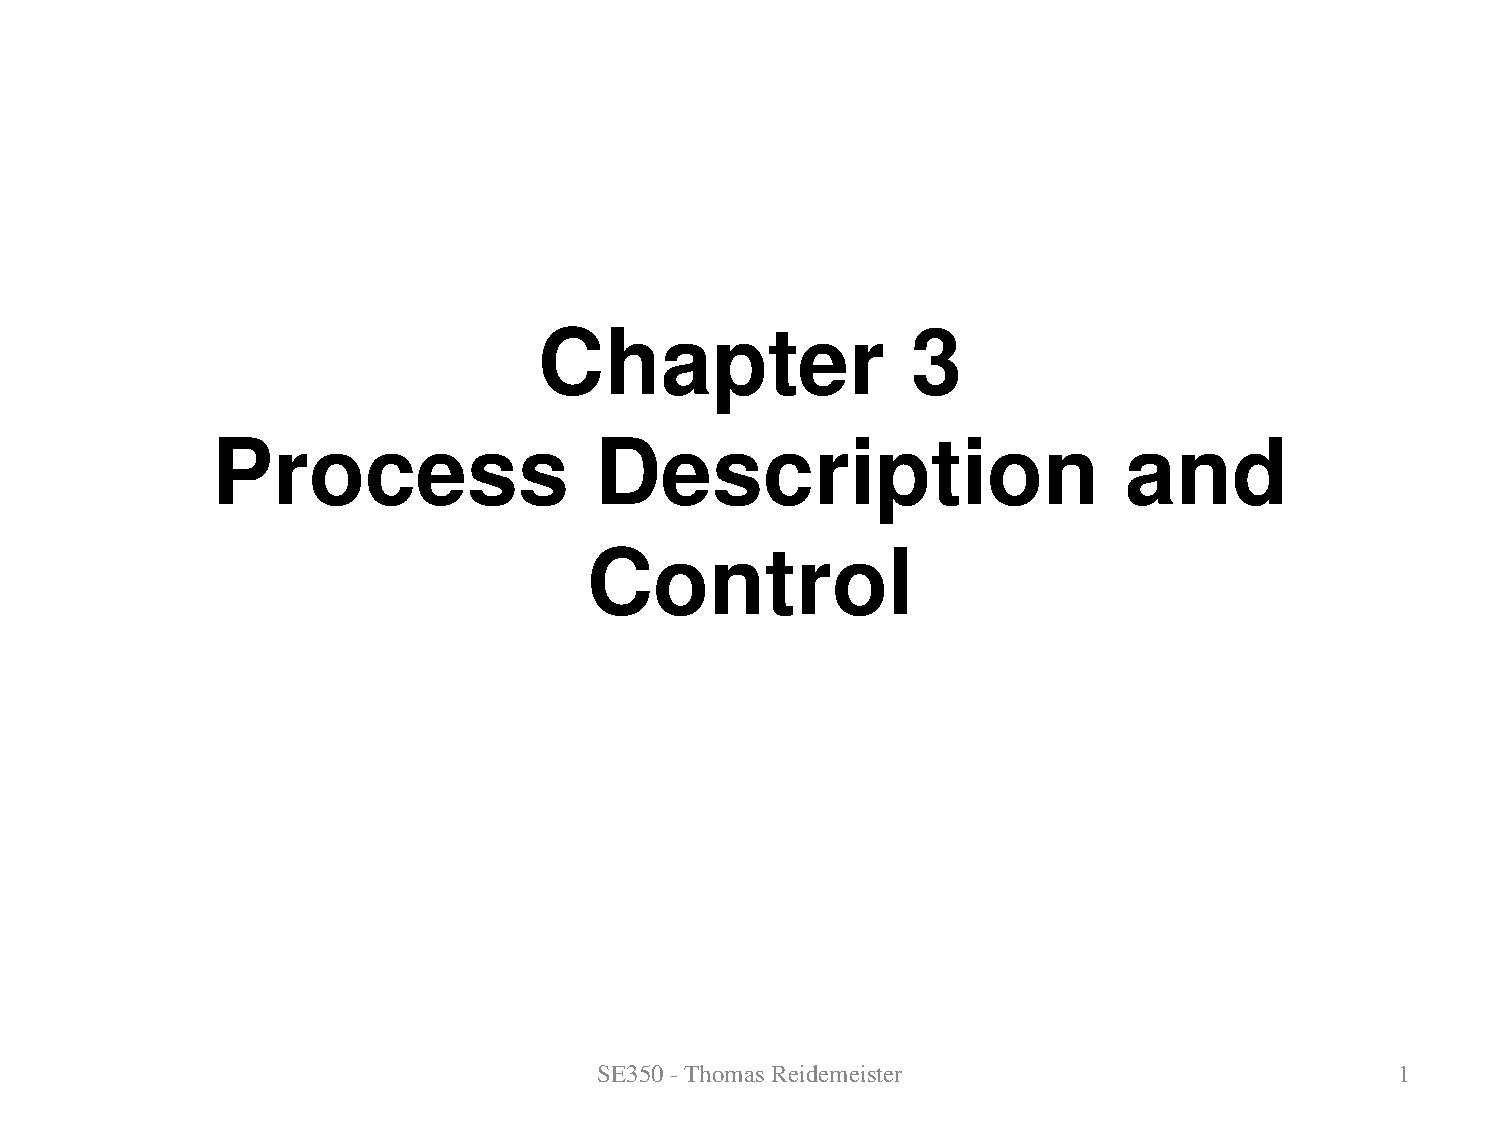
\includepdf[page=45]{03.pdf}
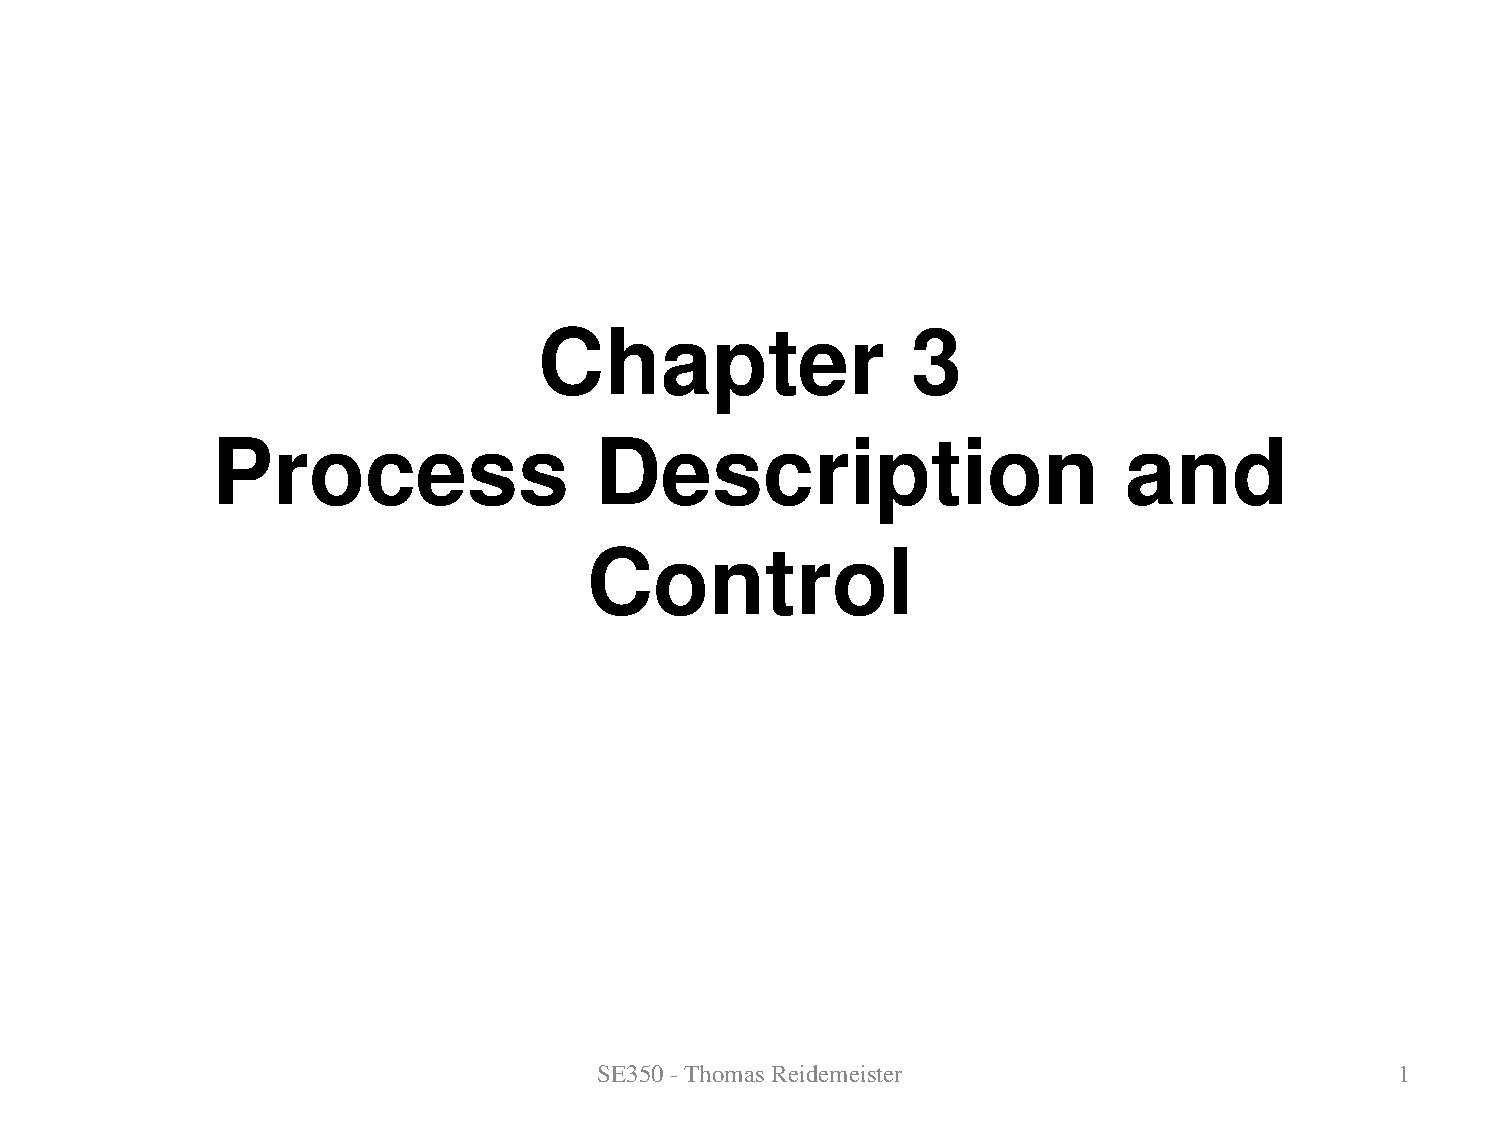
\includepdf[page=46]{03.pdf}
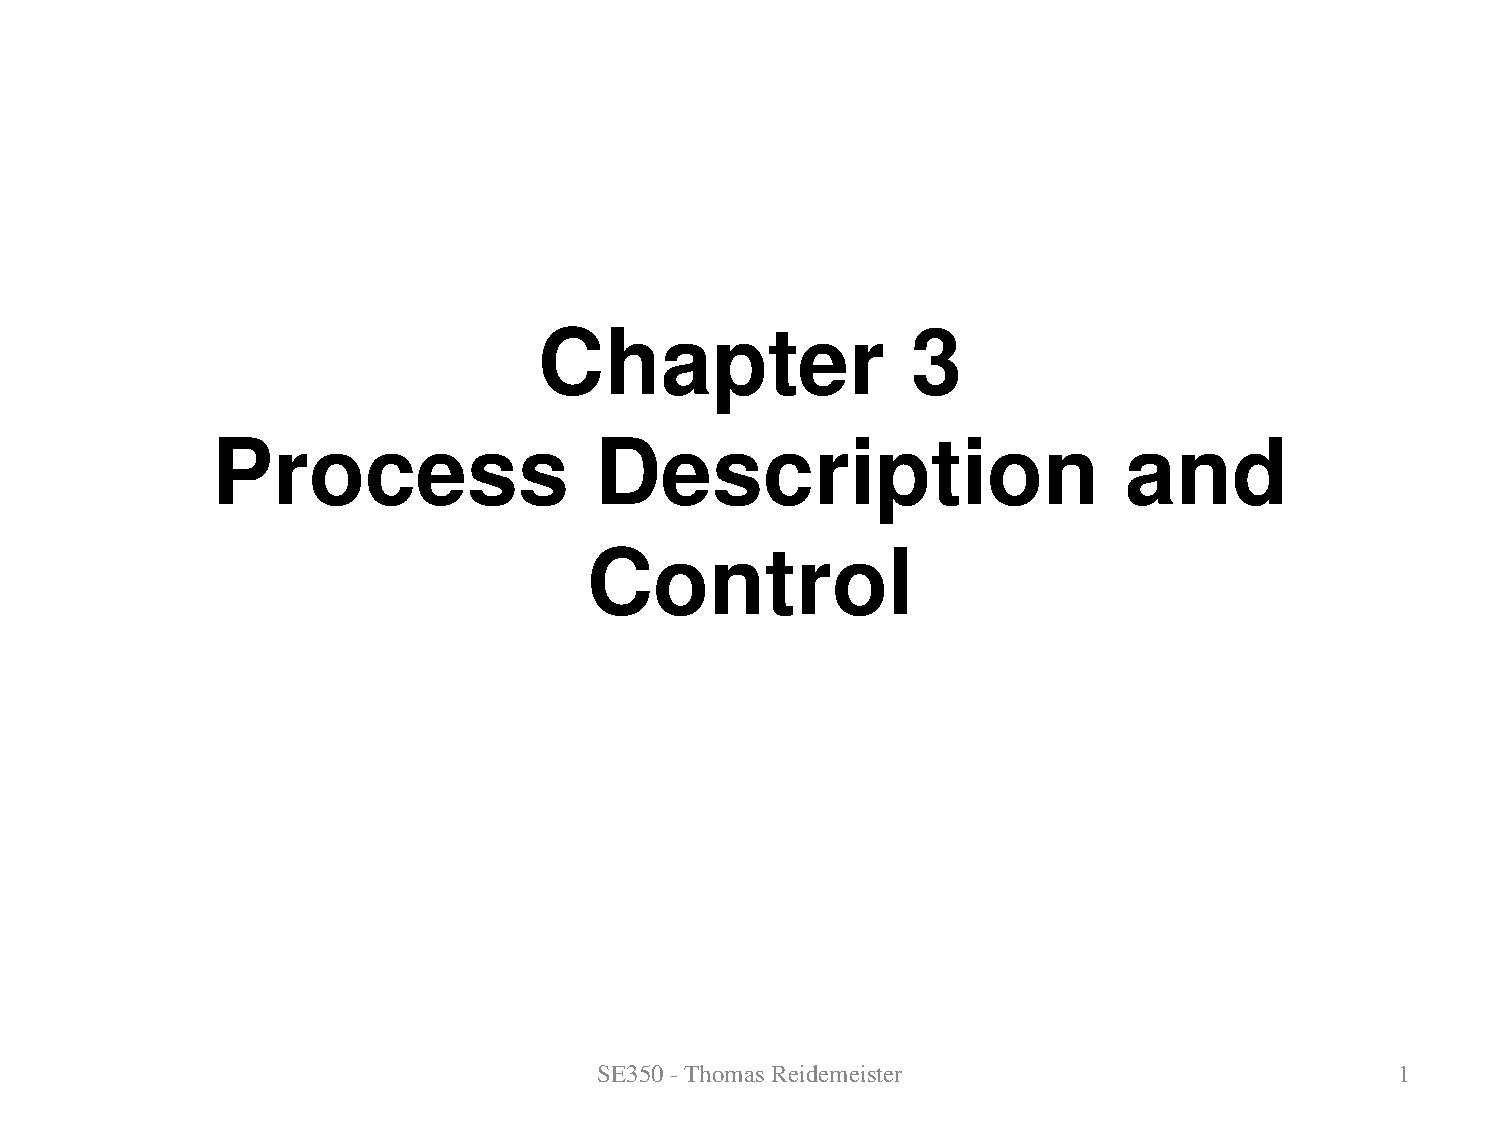
\includepdf[page=47]{03.pdf}
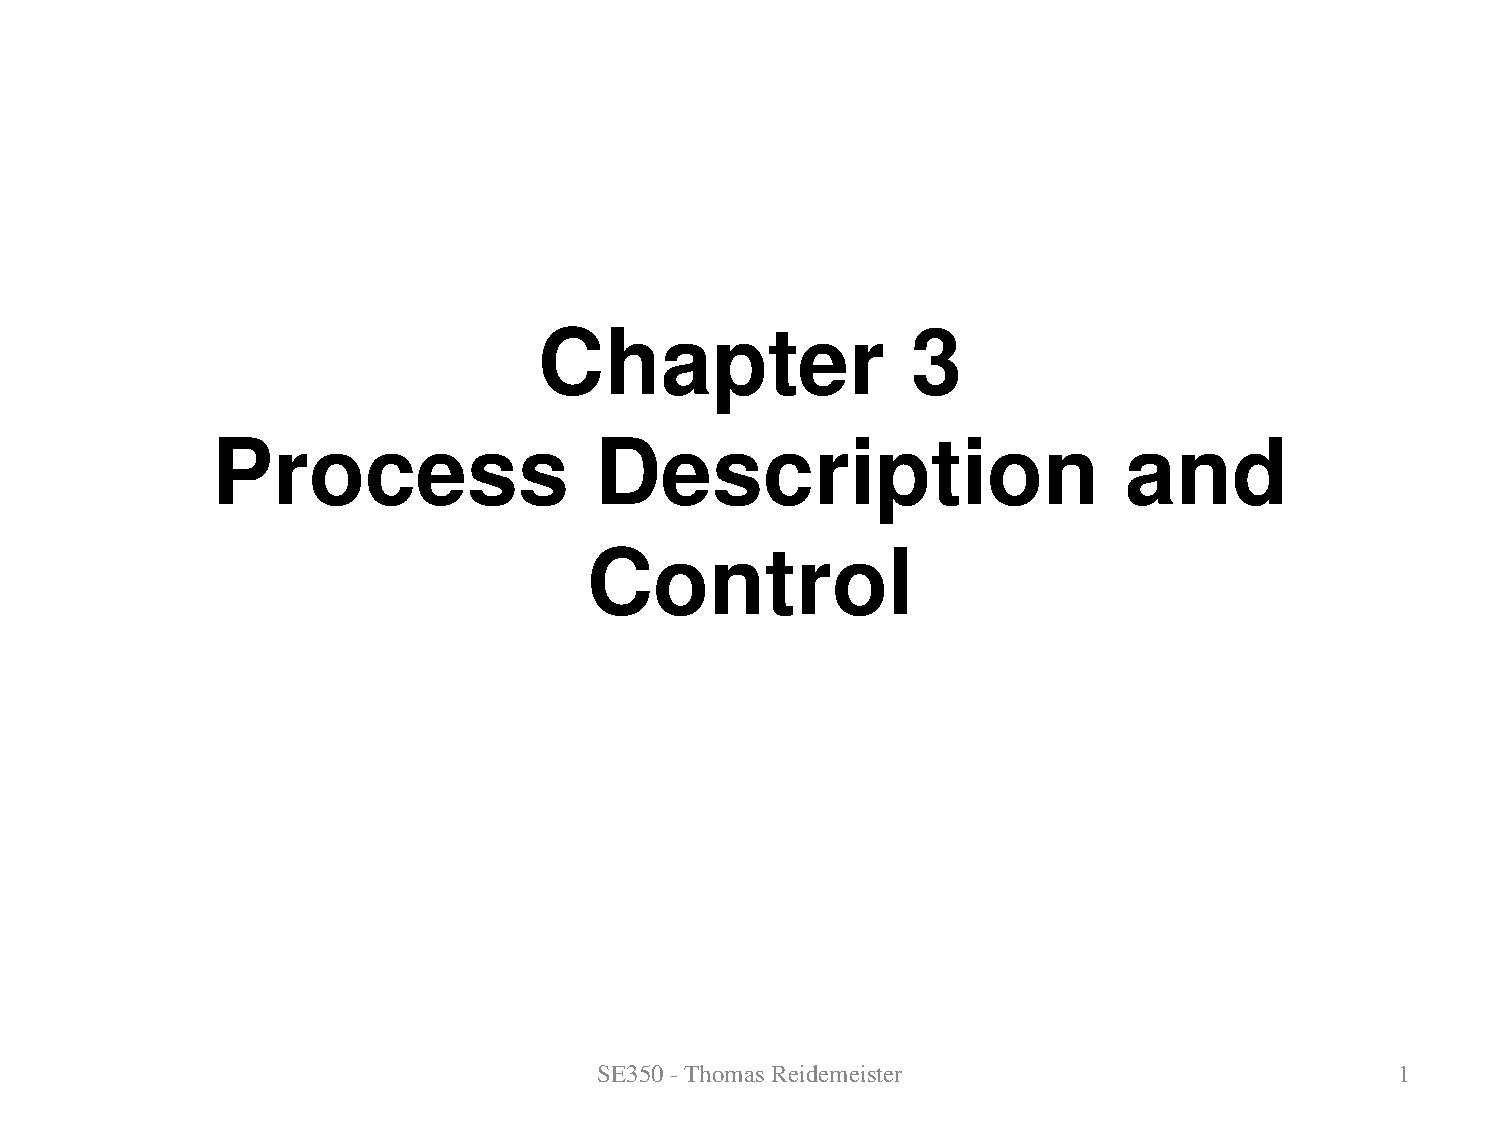
\includepdf[page=48]{03.pdf}
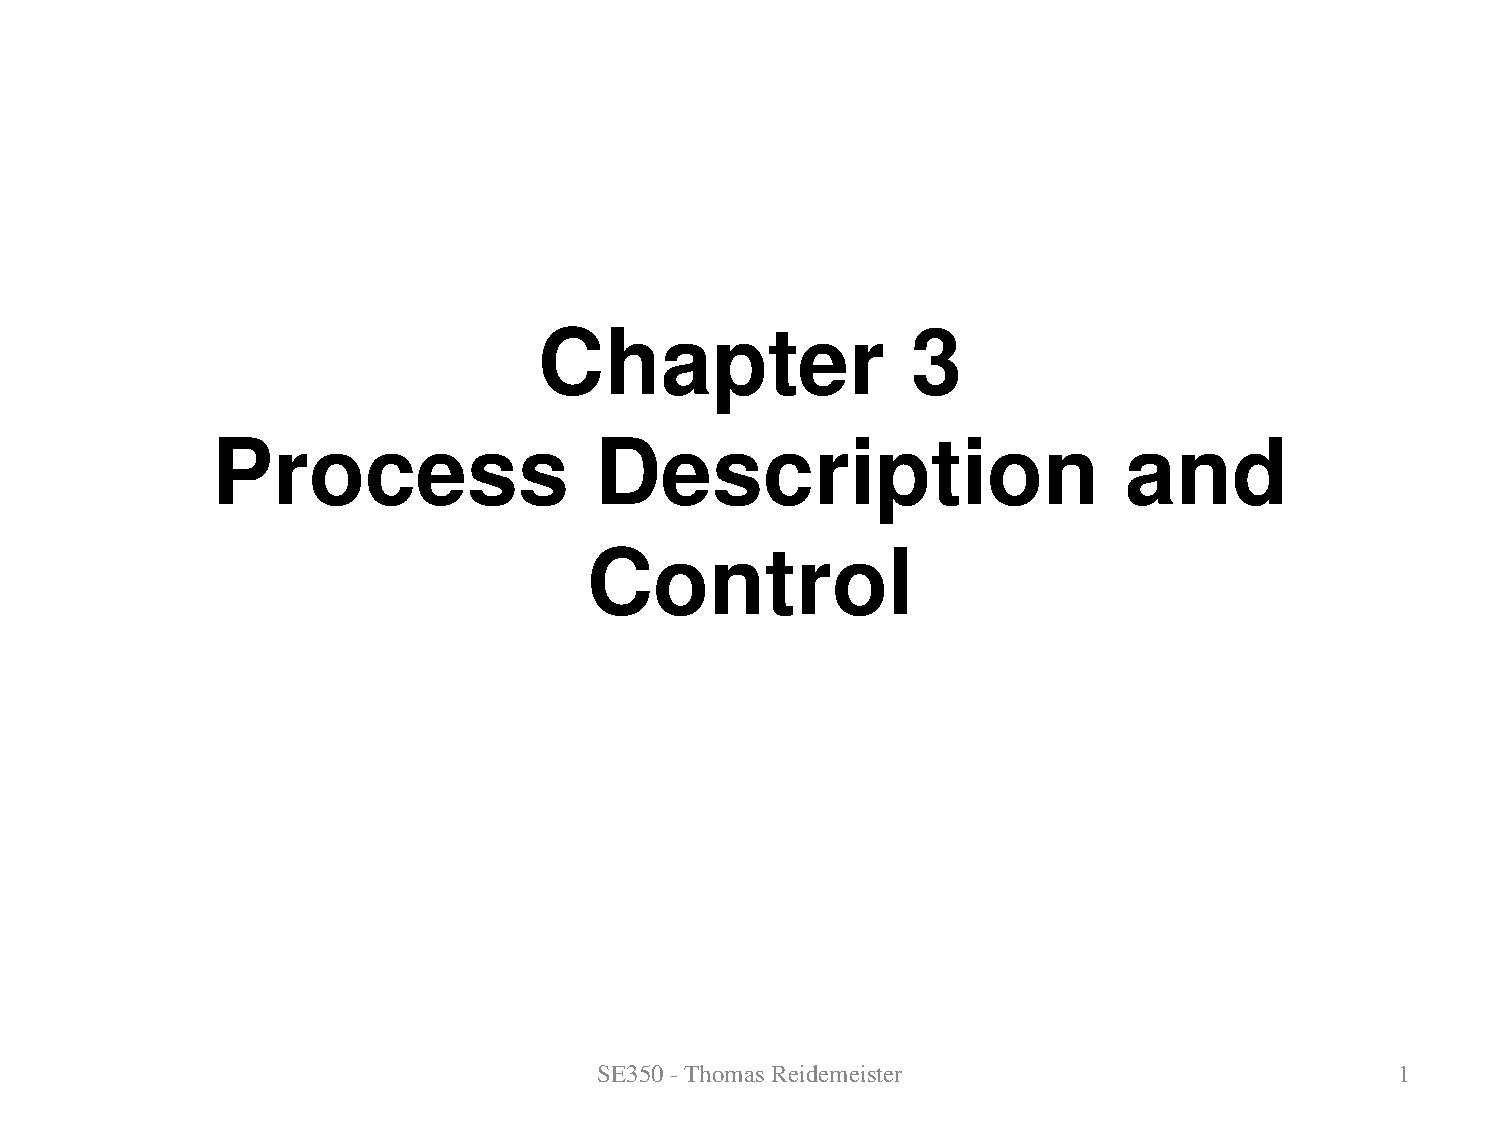
\includepdf[page=49]{03.pdf}
Processor State: All user visible registers (8-34 of them, we work with 16), Control and Status Registers ( PC, condition codes, statuses, misc other things), Stack Pointers (where we store parameters, two kinds system and user stacks), Scheduling and State information, bunch of other things (see all previous slides).
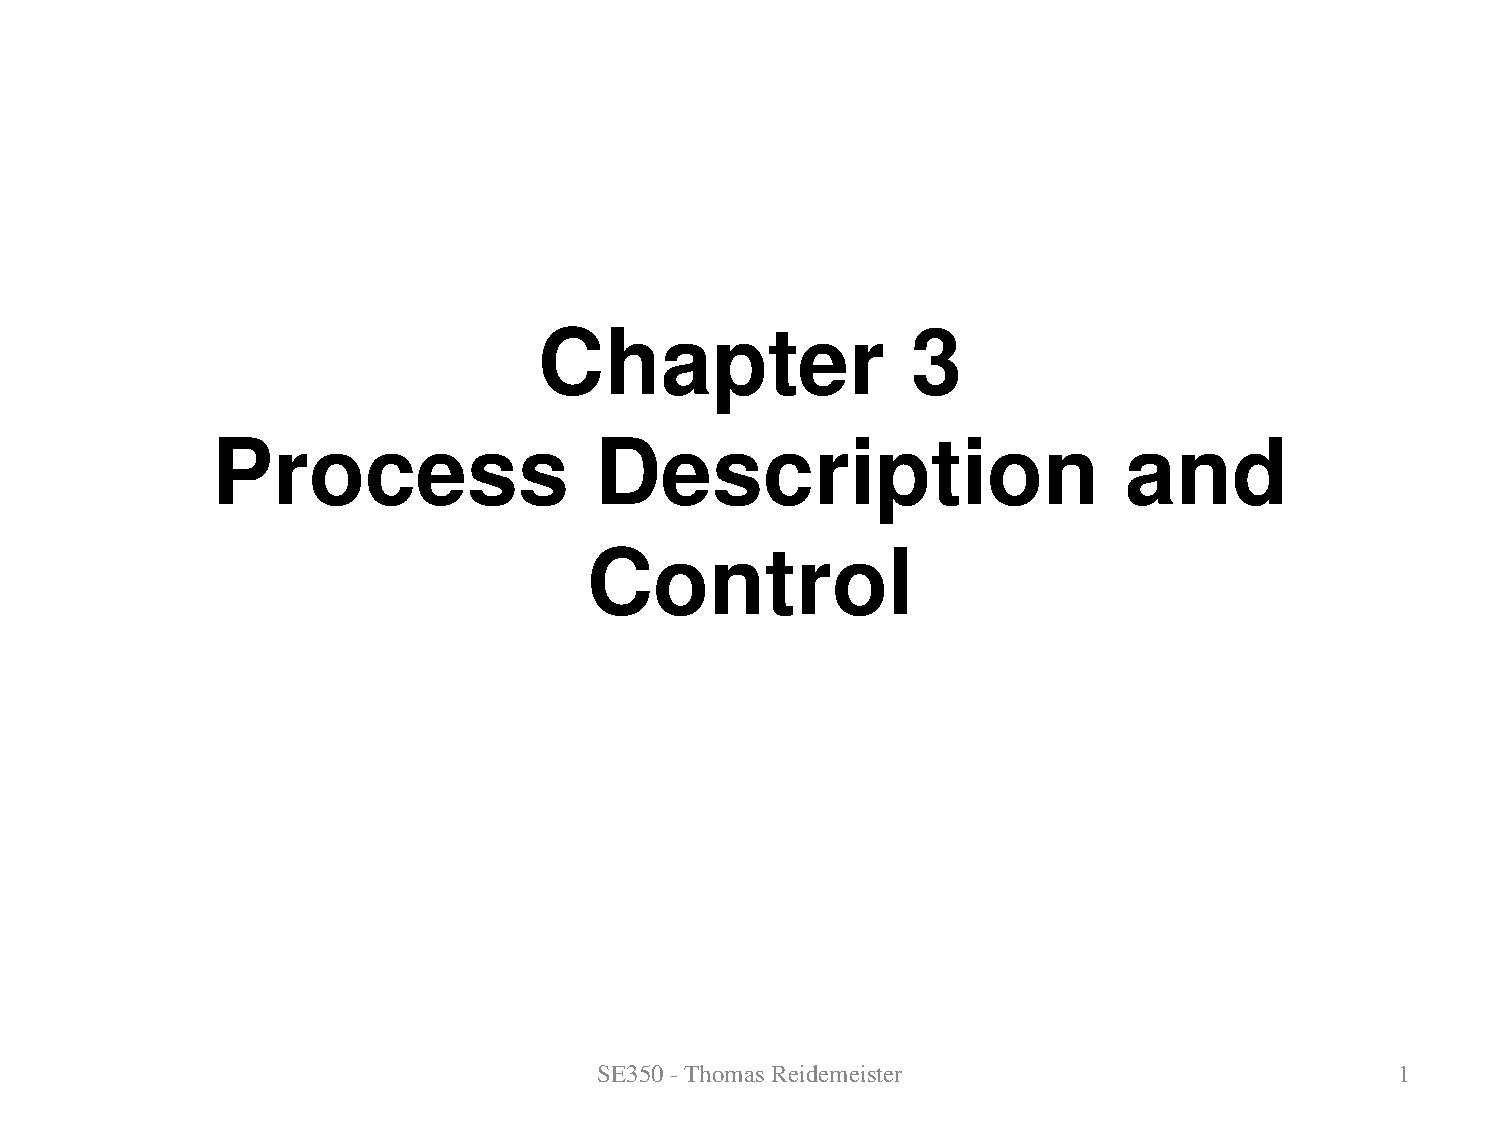
\includepdf[page=50]{03.pdf}
\includepdf[page=51]{03.pdf}
\includepdf[page=52]{03.pdf}
\includepdf[page=53]{03.pdf}
\includepdf[page=54]{03.pdf}
\includepdf[page=55]{03.pdf}
\includepdf[page=56]{03.pdf}
\includepdf[page=57]{03.pdf}
Dude skipped the fuck out of the previous slides
\includepdf[page=58]{03.pdf}
\includepdf[page=59]{03.pdf}
\includepdf[page=60]{03.pdf}
\includepdf[page=61]{03.pdf}
\includepdf[page=62]{03.pdf}
\includepdf[page=63]{03.pdf}
\includepdf[page=64]{03.pdf}
\includepdf[page=65]{03.pdf}
\includepdf[page=66]{03.pdf}
\includepdf[page=67]{03.pdf}
\includepdf[page=68]{03.pdf}
\includepdf[page=69]{03.pdf}
\includepdf[page=70]{03.pdf}
\includepdf[page=71]{03.pdf}
\includepdf[page=72]{03.pdf}
\includepdf[page=73]{03.pdf}
\includepdf[page=74]{03.pdf}
\includepdf[page=75]{03.pdf}
\includepdf[page=76]{03.pdf}
\includepdf[page=77]{03.pdf}
\includepdf[page=78]{03.pdf}
Memorize the fuck out of this process. Seriously. Know it.
\includepdf[page=79]{03.pdf}
\includepdf[page=80]{03.pdf}
A mode switch is when you request something from the processor and continue with the same process when done without the help of the scheduler.
\includepdf[page=81]{03.pdf}
We can implement our OS using two stack pointers and switch between the two when mode changes to strictly ensure isolation of modes.
\includepdf[page=82]{03.pdf}
This is the third way to implement an OS. This is good for multitiered OS and works on message passing.
\includepdf[page=83]{03.pdf}
This is pretty good for reliability since we can just restart processes that fail instead and exploding.


\end{document}
